\begin{document}

\mode<presentation>{
\title{Introduction to Quantum Computing and Spin Networks}
\author{dln-dev}
\date{February 13th 2017}
%\logo{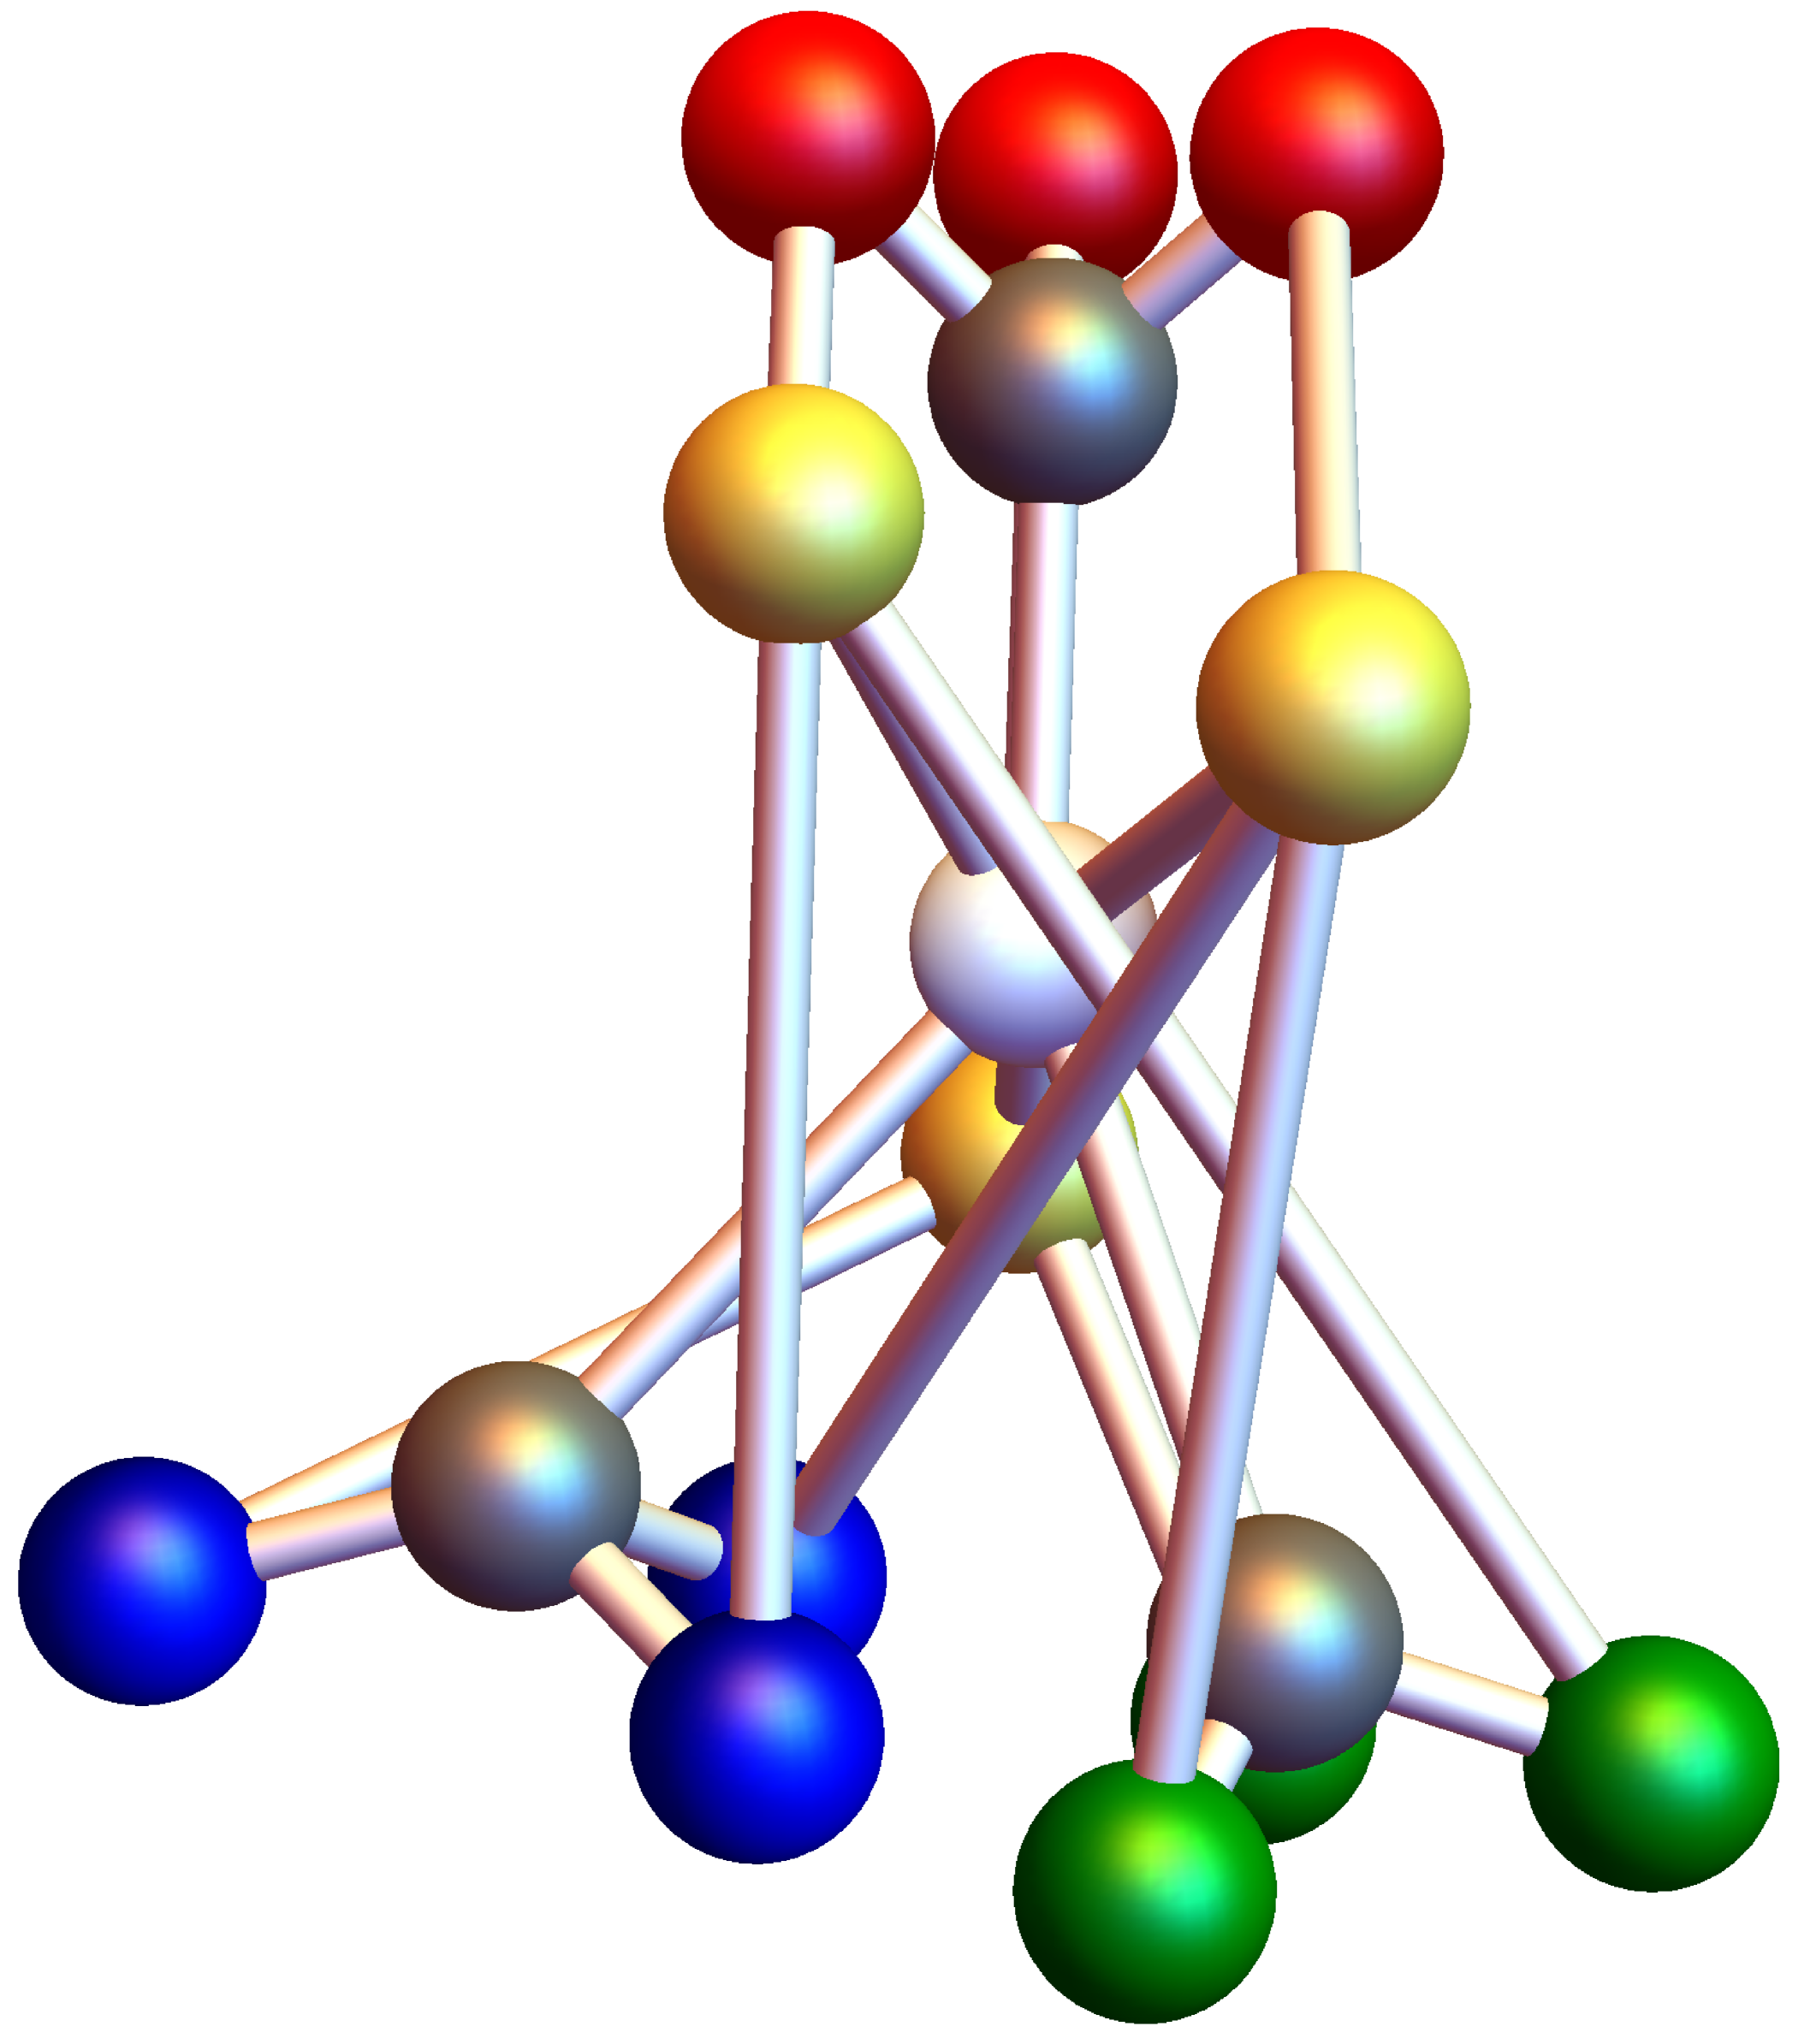
\includegraphics[width=\textwidth]{Images/switch_square}}
\titlegraphic{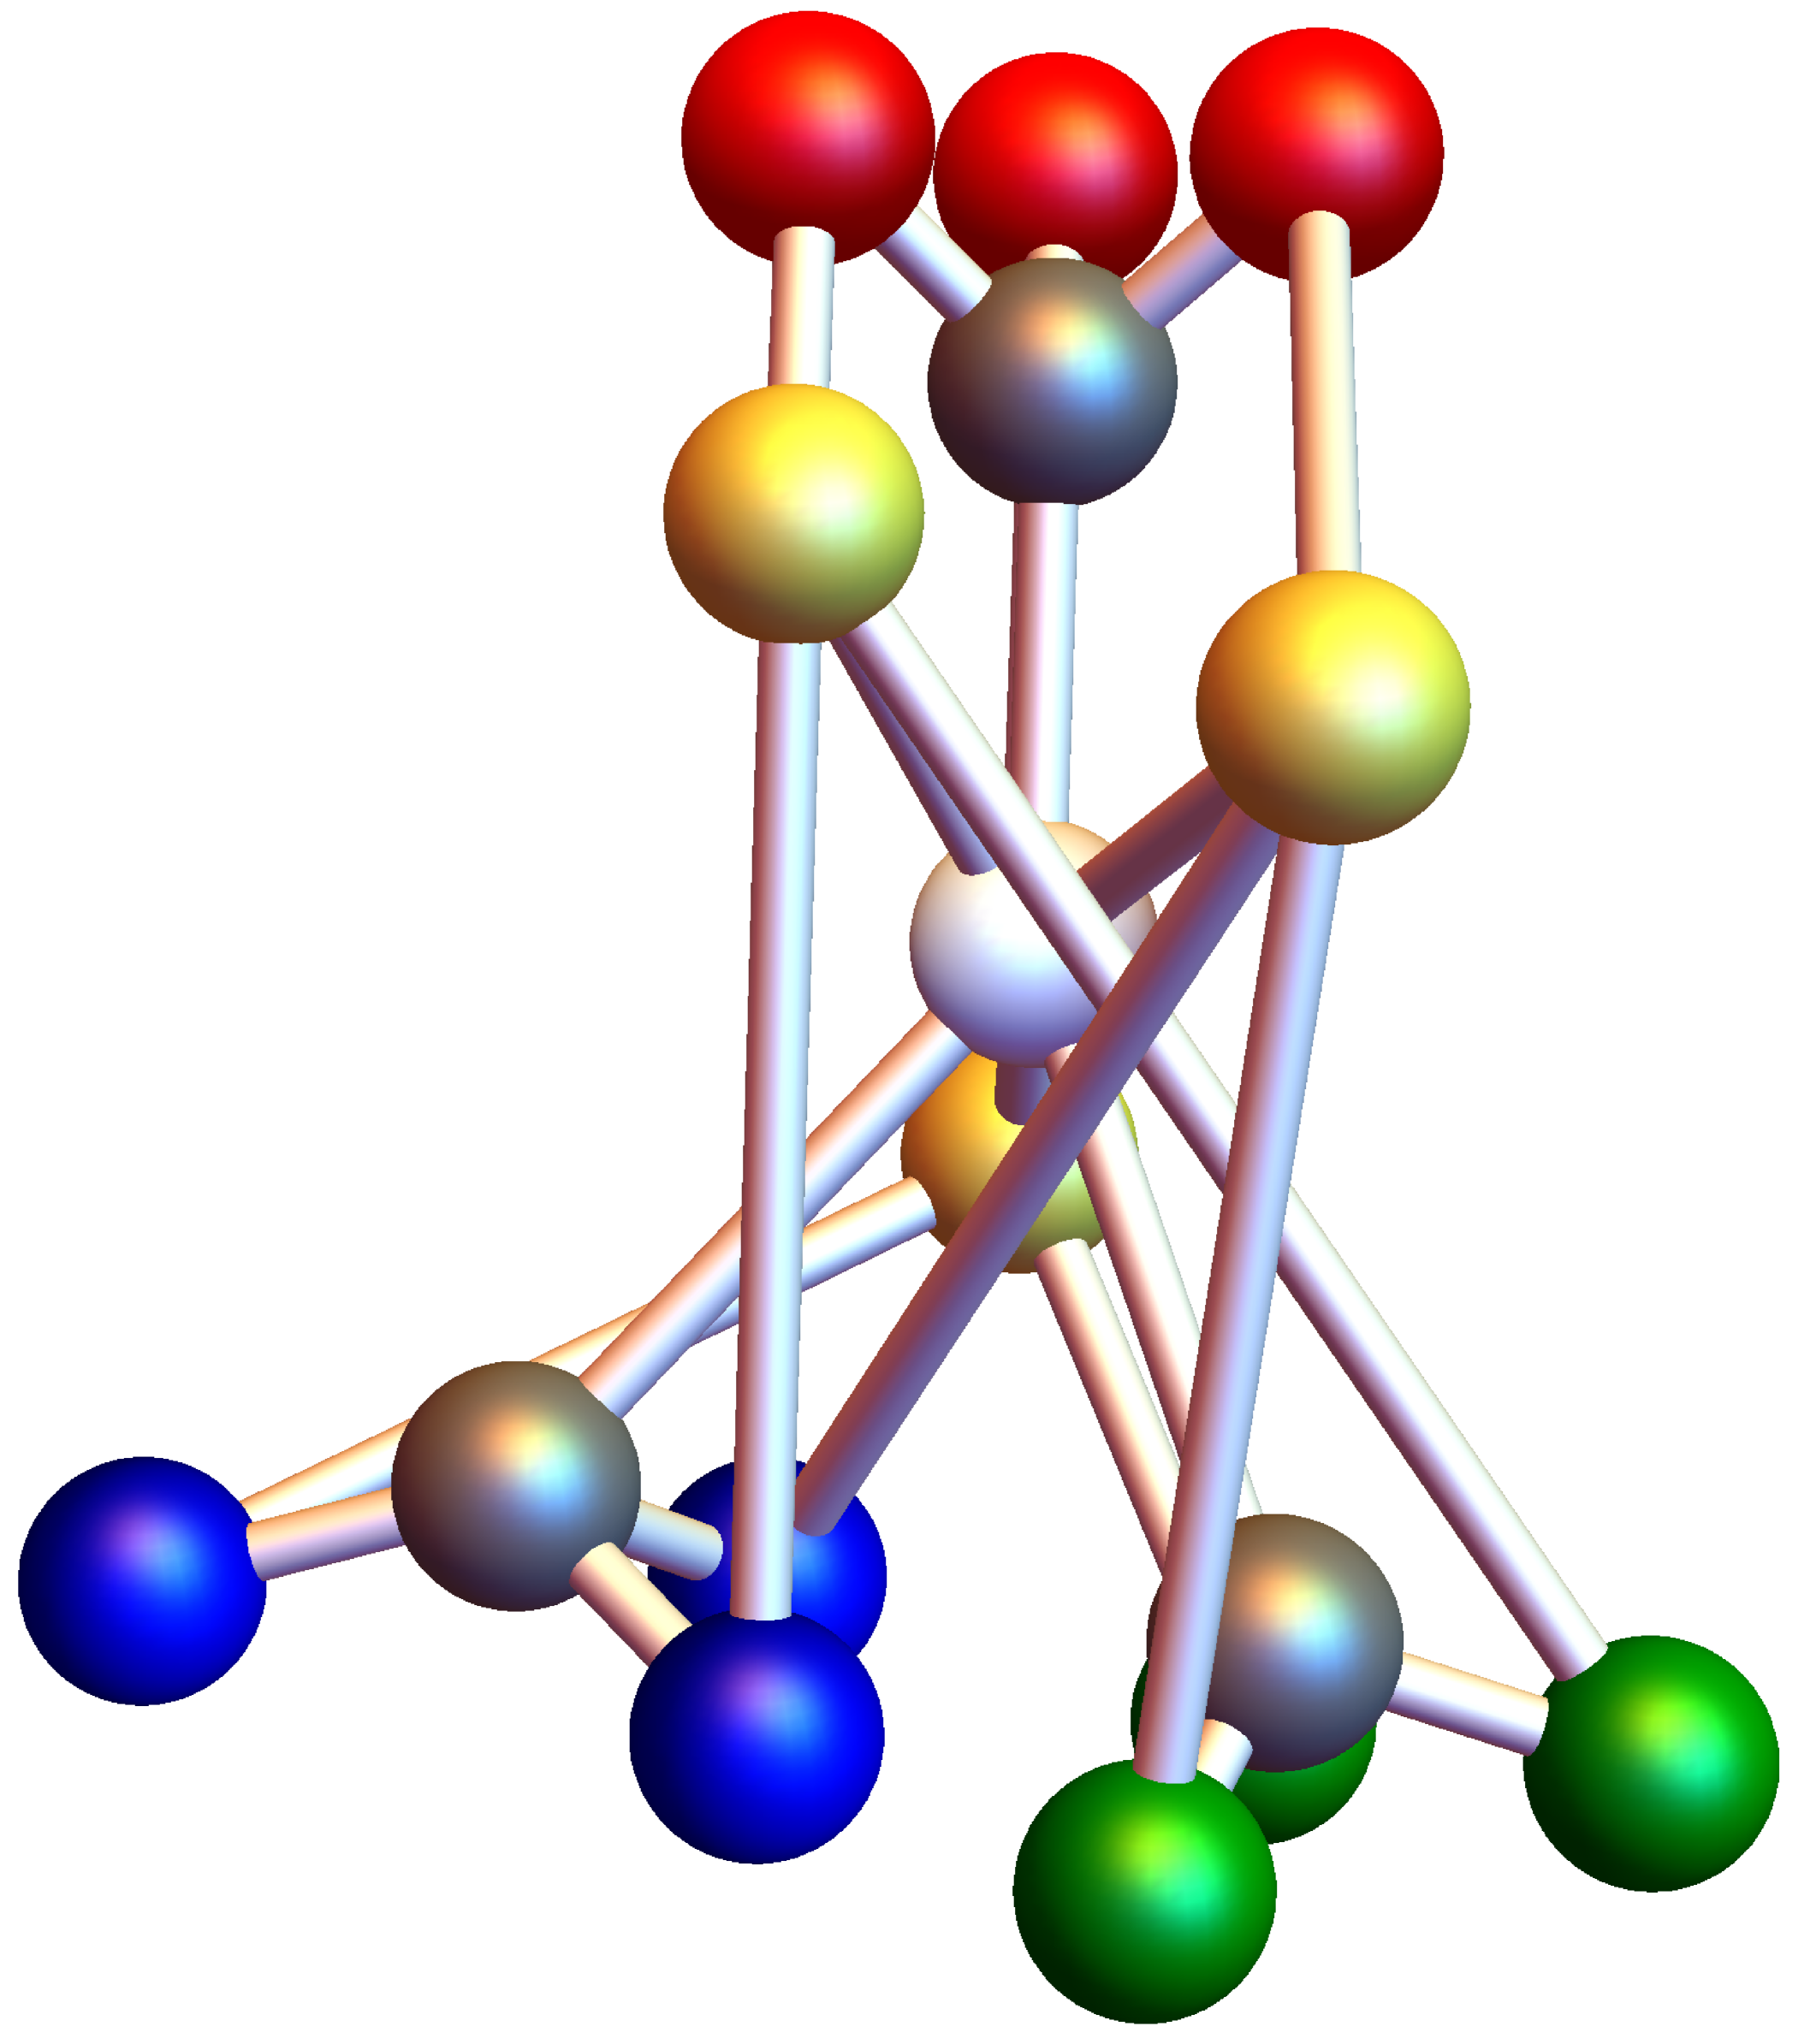
\includegraphics[width=0.1\textwidth]{Images/switch_square}}

\frame{\titlepage}
}

\mode<article>{\begin{titlepage}
	\center
	\vspace*{5.0cm}
	{ \huge \bfseries Introduction to Quantum Computing and Spin Networks}\\[0.4cm]

	\textsc{\Large dln-dev}\\[1.5cm]
	{\large February 13th 2017}\\[5.0cm]

	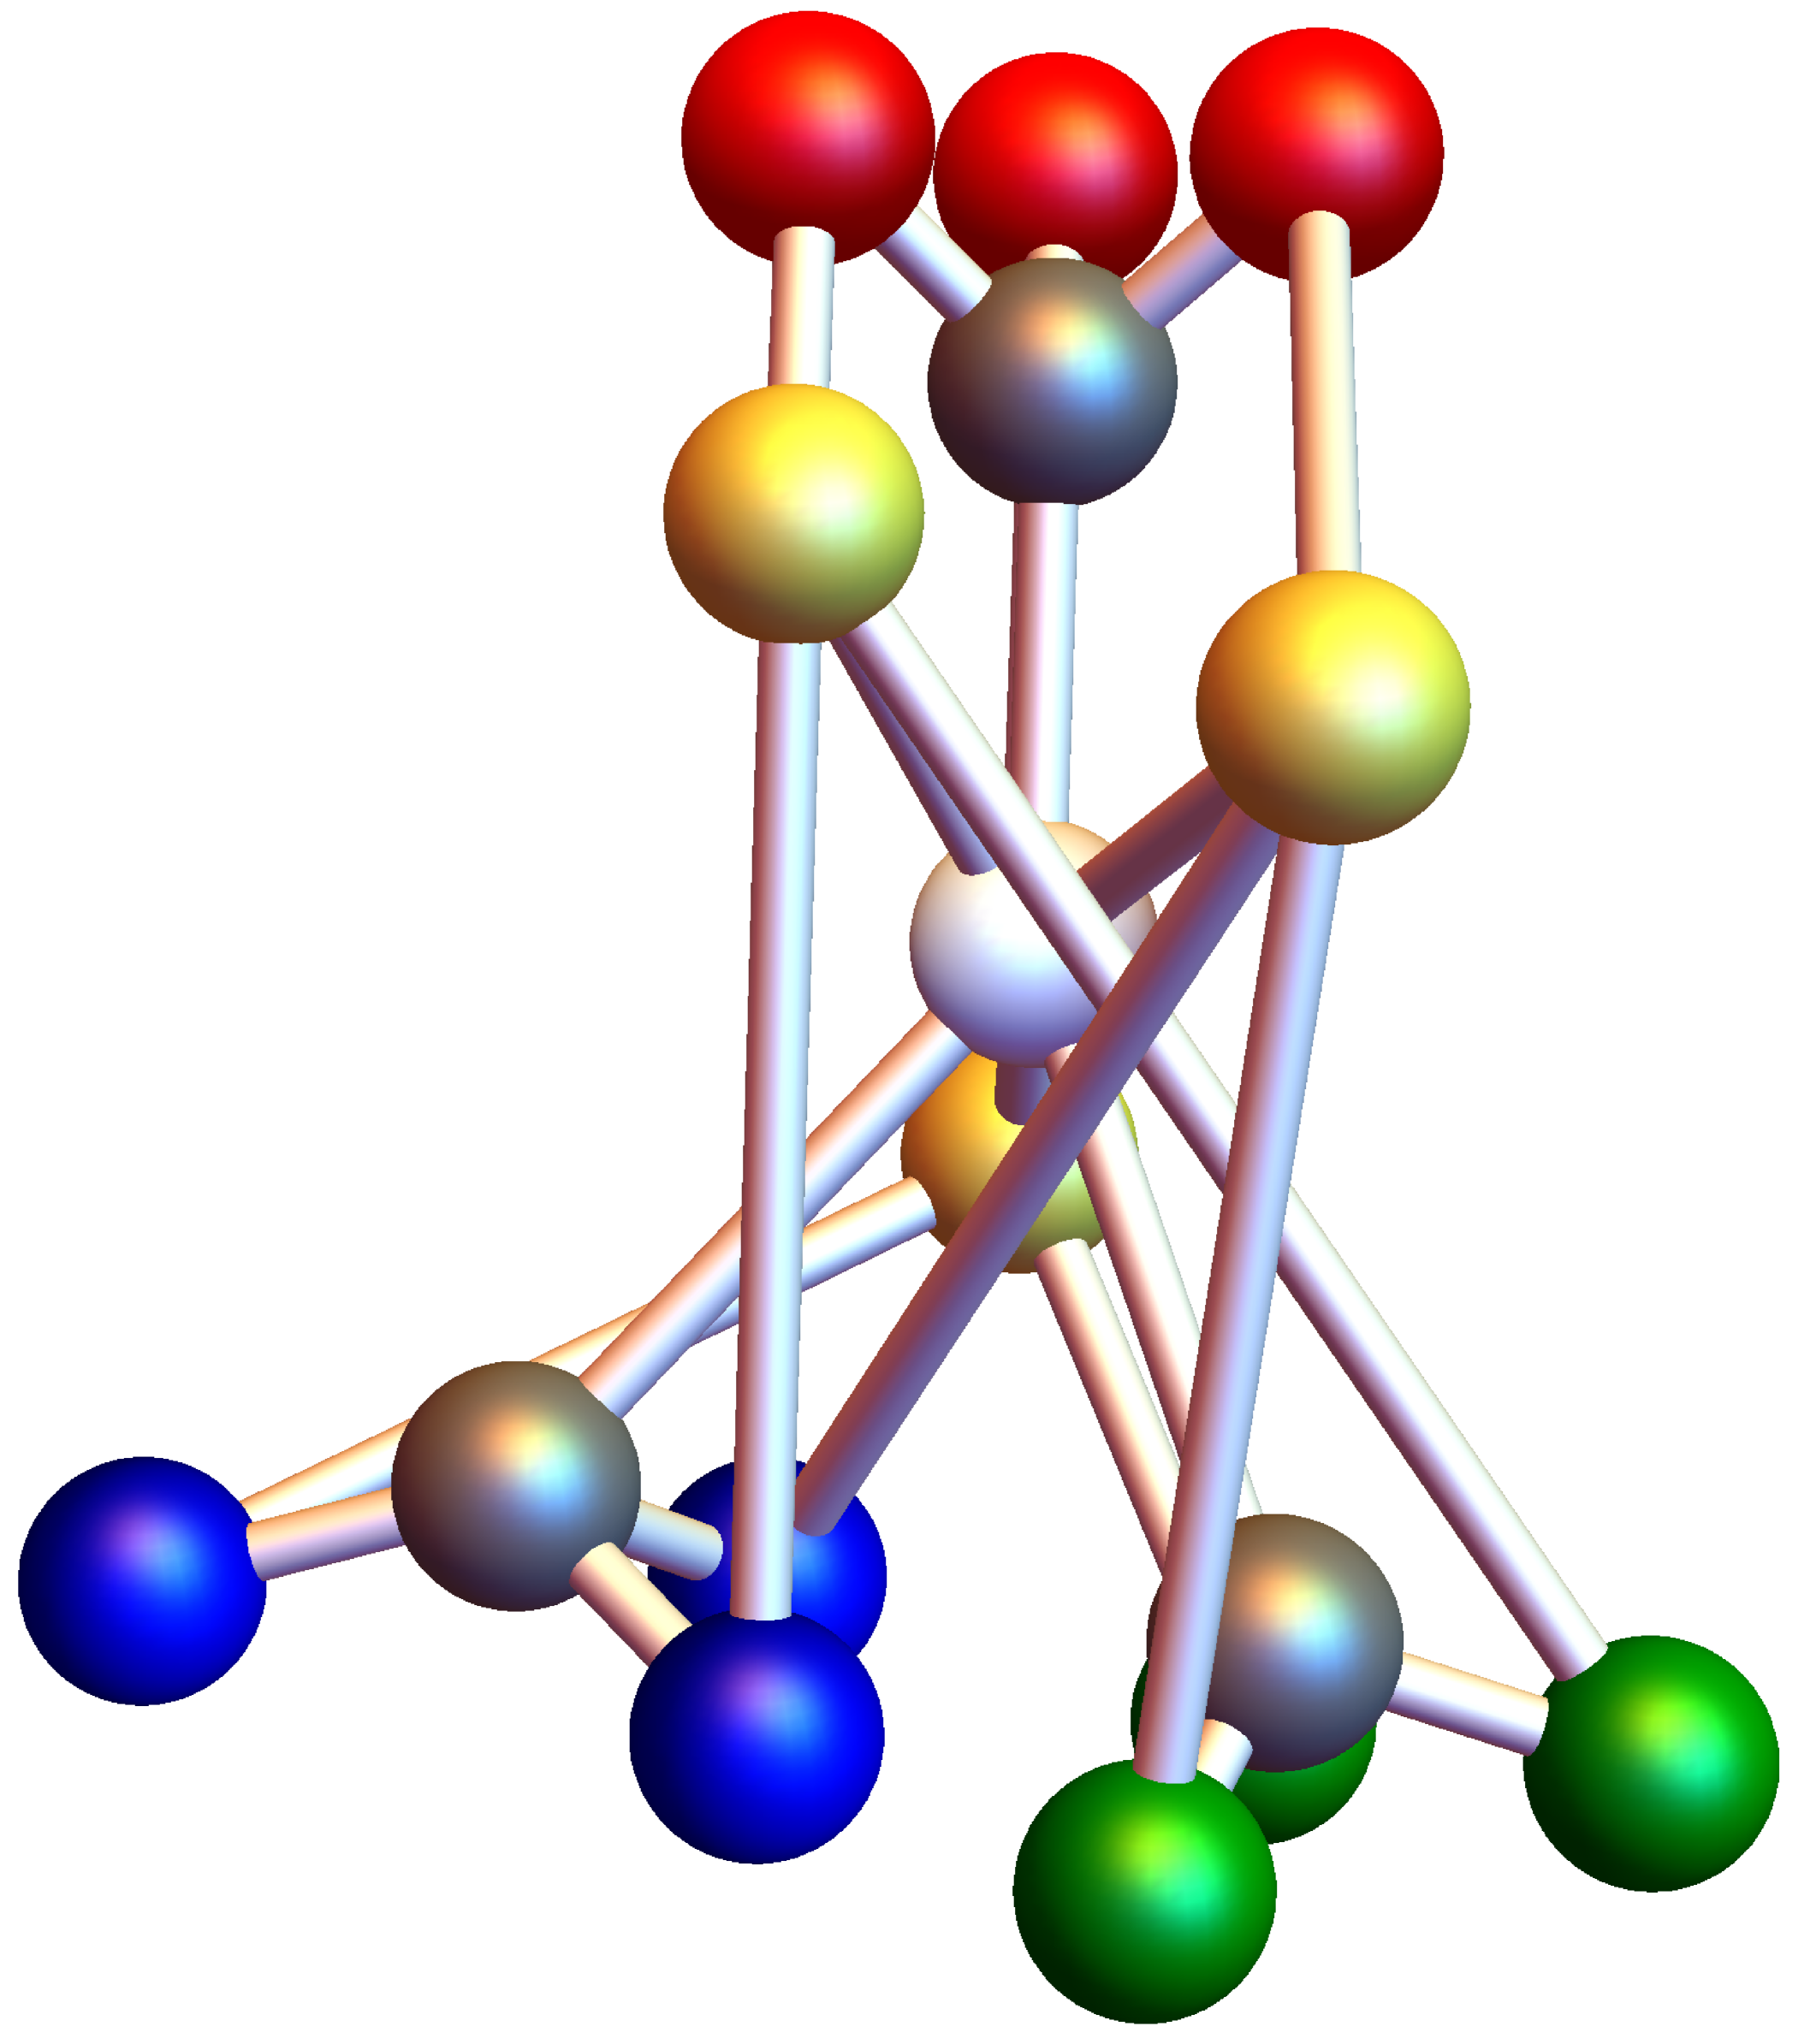
\includegraphics[width=0.3\textwidth]{Images/switch_square}\\[1cm]
	\vfill
\end{titlepage}

\tableofcontents}


\section{Classical Computation}

\subsection{Of Bits and Bytes}
\mode<presentation>{\begin{frame}{Of Bits and Bytes}\label{register}
	\begin{columns}[T]
		\begin{column}{0.5\textwidth}
			\centering\vspace*{1.0cm}
   			\begin{itemize}
   				\item Computers operate on \textsc{registers}
   				\item Composed of $n$ switches $\rightarrow$ \textsc{bits}
   				\item Two discrete states per switch, \textsc{on} and \textsc{off}
   				\item Represents numbers between $0$ and $2^n$
   			\end{itemize}
		\end{column}
		\begin{column}{0.5\textwidth}
			\centering
    		\includegraphics[trim=0 0 0 -40mm, width=\textwidth]{Images/register}
		\end{column}
	\end{columns}
\end{frame}}

\begin{center}
	\includeslide{register}
\end{center}

\noindent text 

\subsection{Turing Machine}
\mode<presentation>{\begin{frame}{Turing Machine}\label{turing}
	\begin{columns}[T]
		\begin{column}{0.5\textwidth}
			\centering\vspace*{1.0cm}
   			\begin{itemize}
   				\item Algorithmic read/write head and register
   				\item Reads one \textsc{bit}
   				\item Manipulates current \textsc{bit} according to program
   			\end{itemize}
		\end{column}
		\begin{column}{0.5\textwidth}
			\centering
    		\includegraphics[trim=0 0 0 -20mm, width=\textwidth]{Images/turingMachine}
		\end{column}
	\end{columns}
\end{frame}}

\begin{center}
	\includeslide{turing}
\end{center}

\noindent text

\subsection{Computational Complexity}
\mode<presentation>{\begin{frame}{Computational Complexity}\label{complexity}
	\begin{columns}[T]
		\begin{column}{0.5\textwidth}
			\centering\vspace*{1.0cm}
   			\begin{itemize}
   				\item Algorithmic read/write head and register
   				\item Reads one \textsc{bit}
   				\item Manipulates current \textsc{bit} according to program
   			\end{itemize}
		\end{column}
		\begin{column}{0.5\textwidth}
			\centering
    		\begin{table}
				\begin{tabular}{l | c | c | c | c }
					Task & Complexity \\
					\hline \hline
					John T & 13:04  \\ 
					Norman P & 8:00 \\
					Multiplication & $\mathcal{O}(n)$ \\
					Factorization & $\mathcal{O}(exp(n^{\log(n)}))$  
				\end{tabular}
			%\caption{Complexity}
			\end{table}
		\end{column}
	\end{columns}
\end{frame}}

\begin{center}
	\includeslide{complexity}
\end{center}

\noindent text

\section{Quantum Computation}
\subsection{Qubits}
\mode<presentation>{\begin{frame}{Qubits}\label{qubits}
	\begin{itemize}
		\item $2$ distinguishable states $\ket{0}$ and $\ket{1}$
		\item Usually spin-$\frac{1}{2}$ systems ($\ket{\uparrow}$ and $\ket{\downarrow}$)
		\item $\ket{0}$ and $\ket{1}$ are basis vectors of the associated \textsc{Hilbert space} $\mathfrak{H}_2$
		\item General state\\
			$\ket{\Psi} = \alpha\ket{0} + \beta\ket{1}$\\
			$\bra{\Psi} = \alpha^*\bra{0} + \beta^*\bra{1}$\\
			with $\alpha, \beta \in \mathbb{C}$
		\item Independent: $\braket{0|1} = 0$, $\braket{1|0} = 0$
	\end{itemize}
\end{frame}}

\begin{center}
	\includeslide{qubits}
\end{center}

\noindent text

\mode<presentation>{\begin{frame}{Measurement}\label{measurement}
	\begin{columns}[T]
		\begin{column}{0.5\textwidth}
			\centering\vspace*{1.0cm}
   			\begin{itemize}
   				\item measurement
   			\end{itemize}
		\end{column}
		\begin{column}{0.5\textwidth}
			\centering
    		\includegraphics[trim=0 0 0 0mm, width=\textwidth]{Images/bloch_sphere}
		\end{column}
	\end{columns}
\end{frame}}

\begin{center}
	\includeslide{PST}
\end{center}

\noindent text

\mode<presentation>{\begin{frame}[t]{Quantum Register}\label{qregister}
	\begin{itemize}
		\item Classically: $N$ systems have $N\cdot f$ coordinates
		\item Quantum: tensor product of individual Hilbert spaces\\
			$\mathfrak{H}^{\text{full}} = \mathfrak{H}_1 \otimes \mathfrak{H}_2 \otimes \dots \otimes \mathfrak{H}_N$\\
			$\rightarrow \text{dim}(\mathfrak{H}^{full}) = 2^N$ 
		\item Basis vectors: \\
			$\ket{0}\otimes\ket{0}, \ket{0}\otimes\ket{1}, \ket{1}\otimes\ket{0}, \ket{1}\otimes\ket{1}$\\
			short: $\ket{00}, \ket{01}, \ket{10}, \ket{11}$
		\item System $2$ in superposition, register state\\
			$\ket{\Psi} = \alpha\ket{0000} + \beta\ket{0100}$
	\end{itemize}
\end{frame}}

\begin{center}
	\includeslide{qregister}
\end{center}

\noindent text

\mode<presentation>{\begin{frame}[t]{Entanglement}\label{entanglement}
	\begin{exampleblock}{}
	\setlength\abovedisplayskip{-8pt}
	\begin{center}
		$a_{ij} = \left\{
	\begin{array}{ll}
		1  & \{i,j\} \in E \\
		0  & \text{otherwise}
	\end{array}
\right.$	
	\end{center}
	\end{exampleblock}
	\begin{itemize}
		\item No multi-edges $\rightarrow$ all elements either $0$ or $1$
		\item Unordered Pairs $\rightarrow$ symmetric
		\item Orthogonal basis exists%, eigenvalues are roots of $det(A-\lambda \text{1}) = 0$
	\end{itemize}
	\begin{columns}[T]
		\begin{column}{0.5\textwidth}
			\centering
   			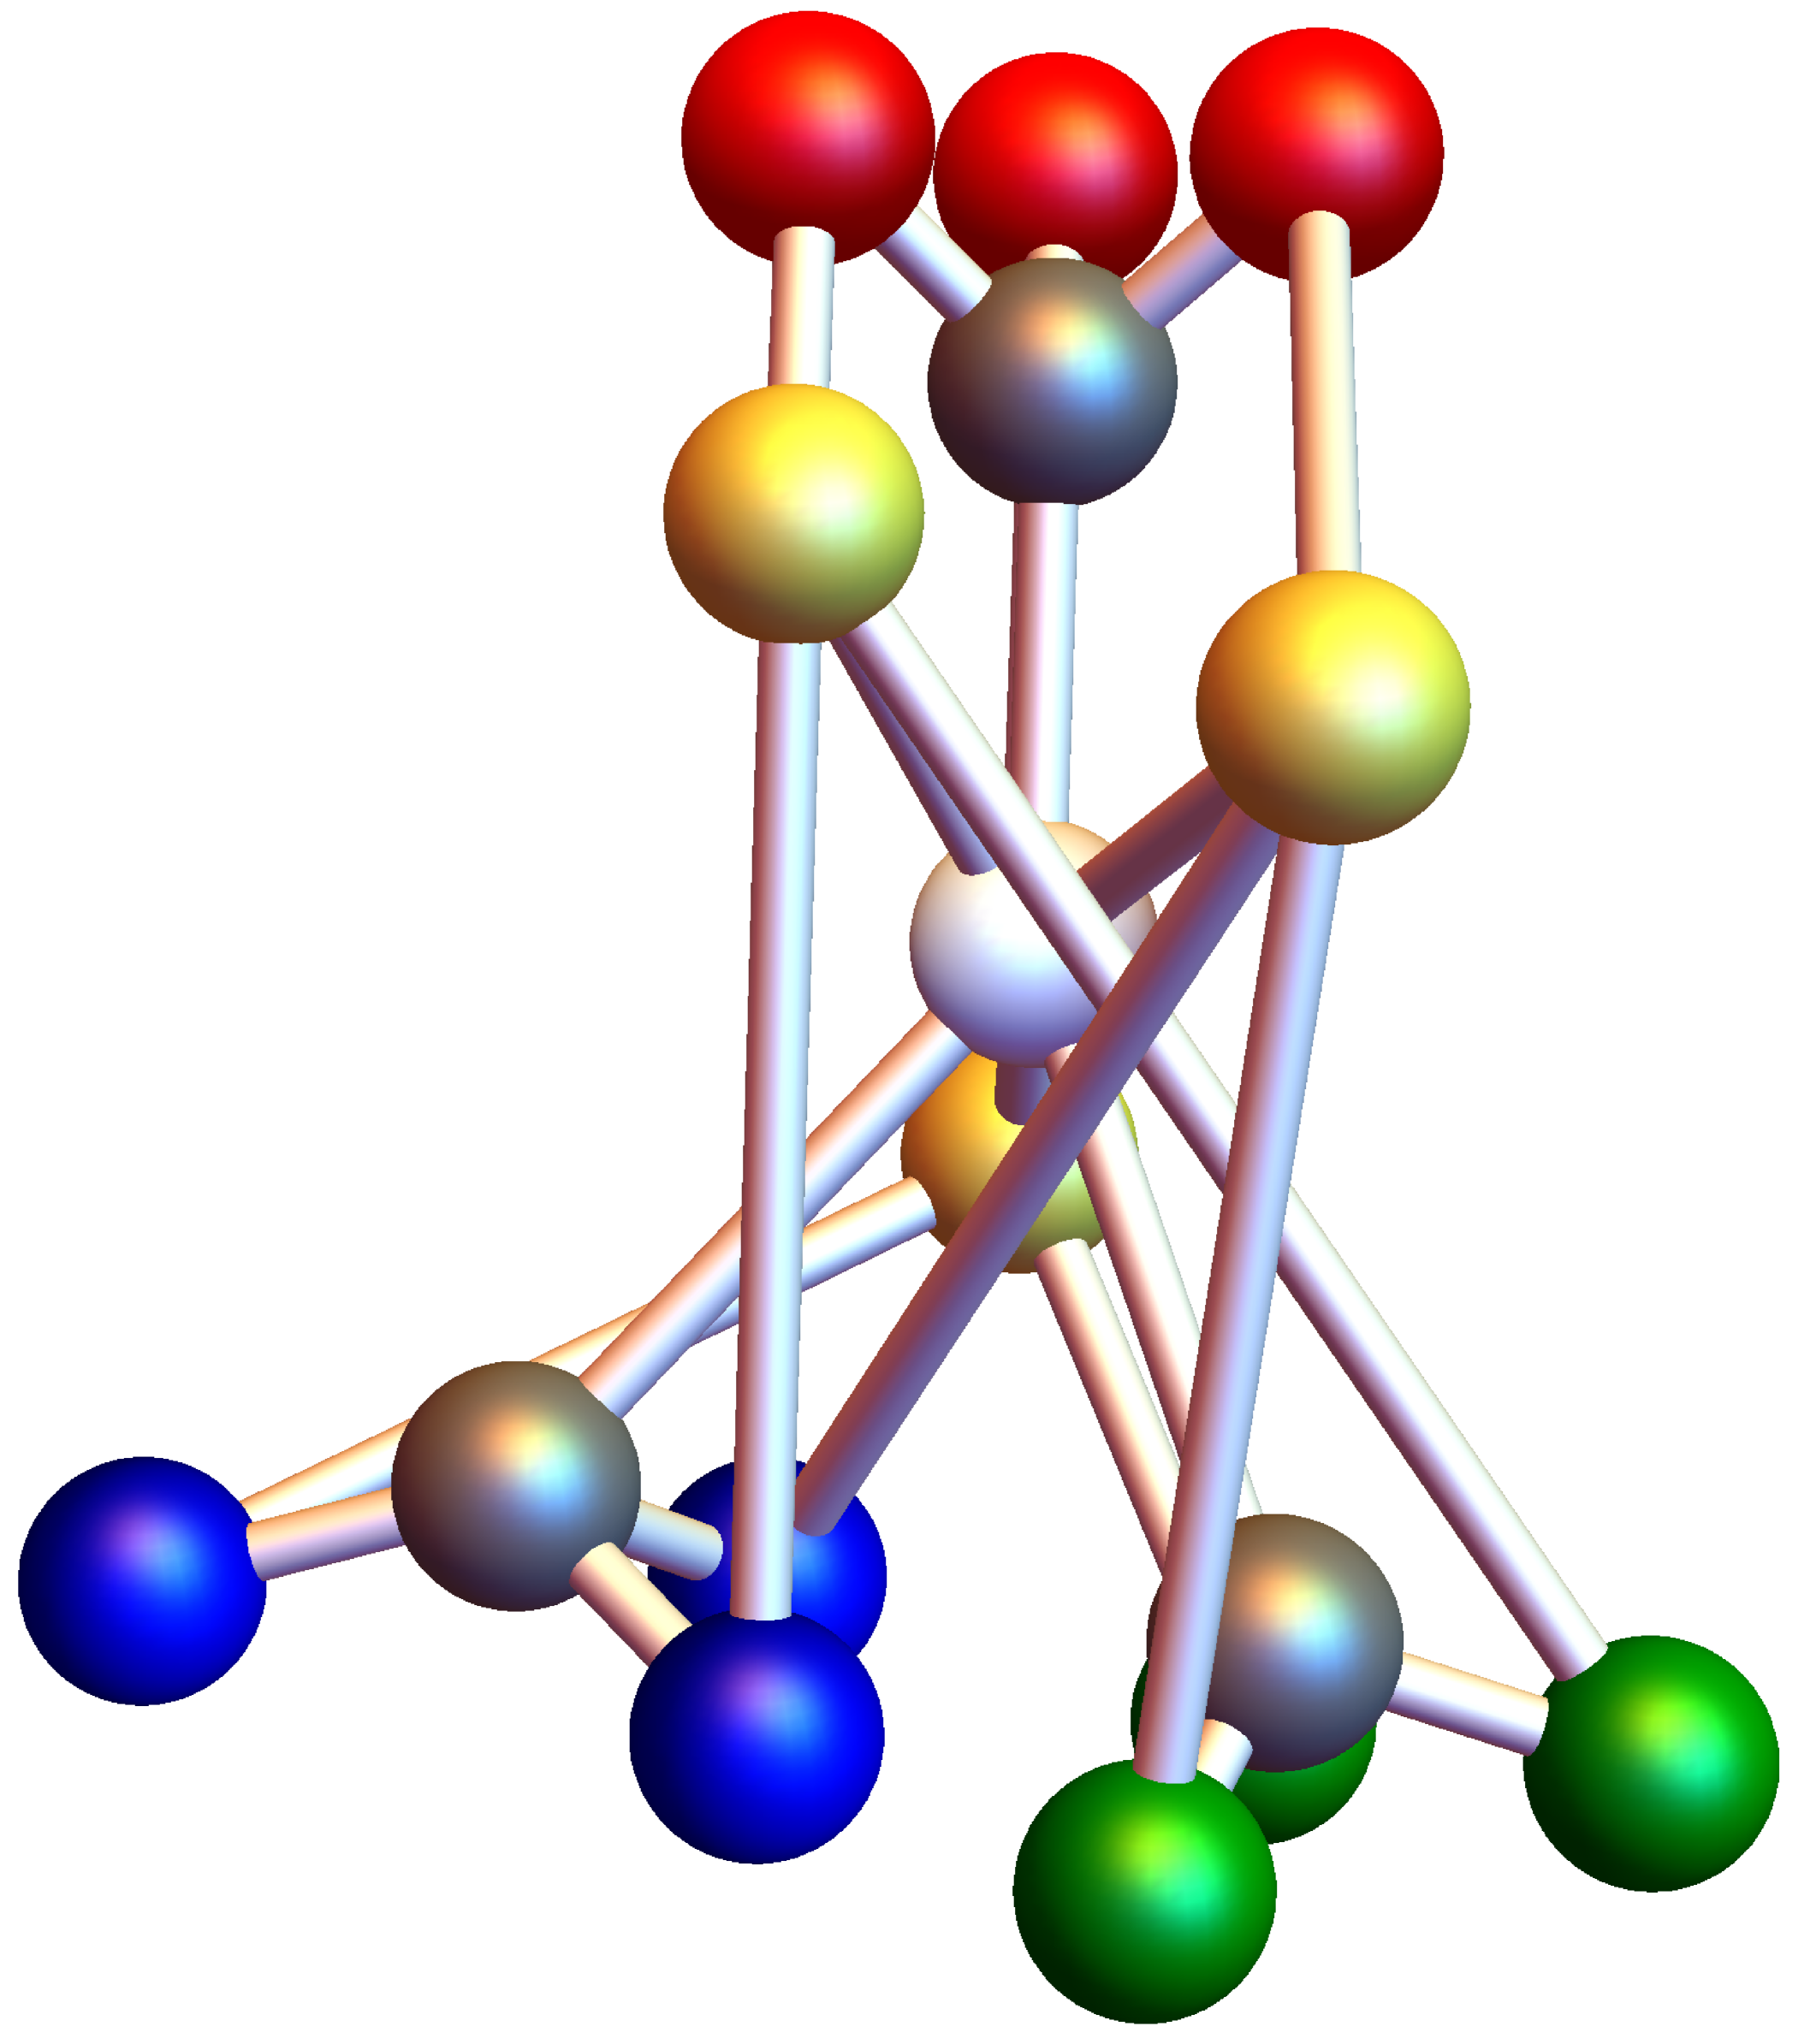
\includegraphics[trim=0 0 0 5mm, width=0.5\textwidth]{Images/switch_square}
		\end{column}
		\begin{column}{0.5\textwidth}
			\centering
    		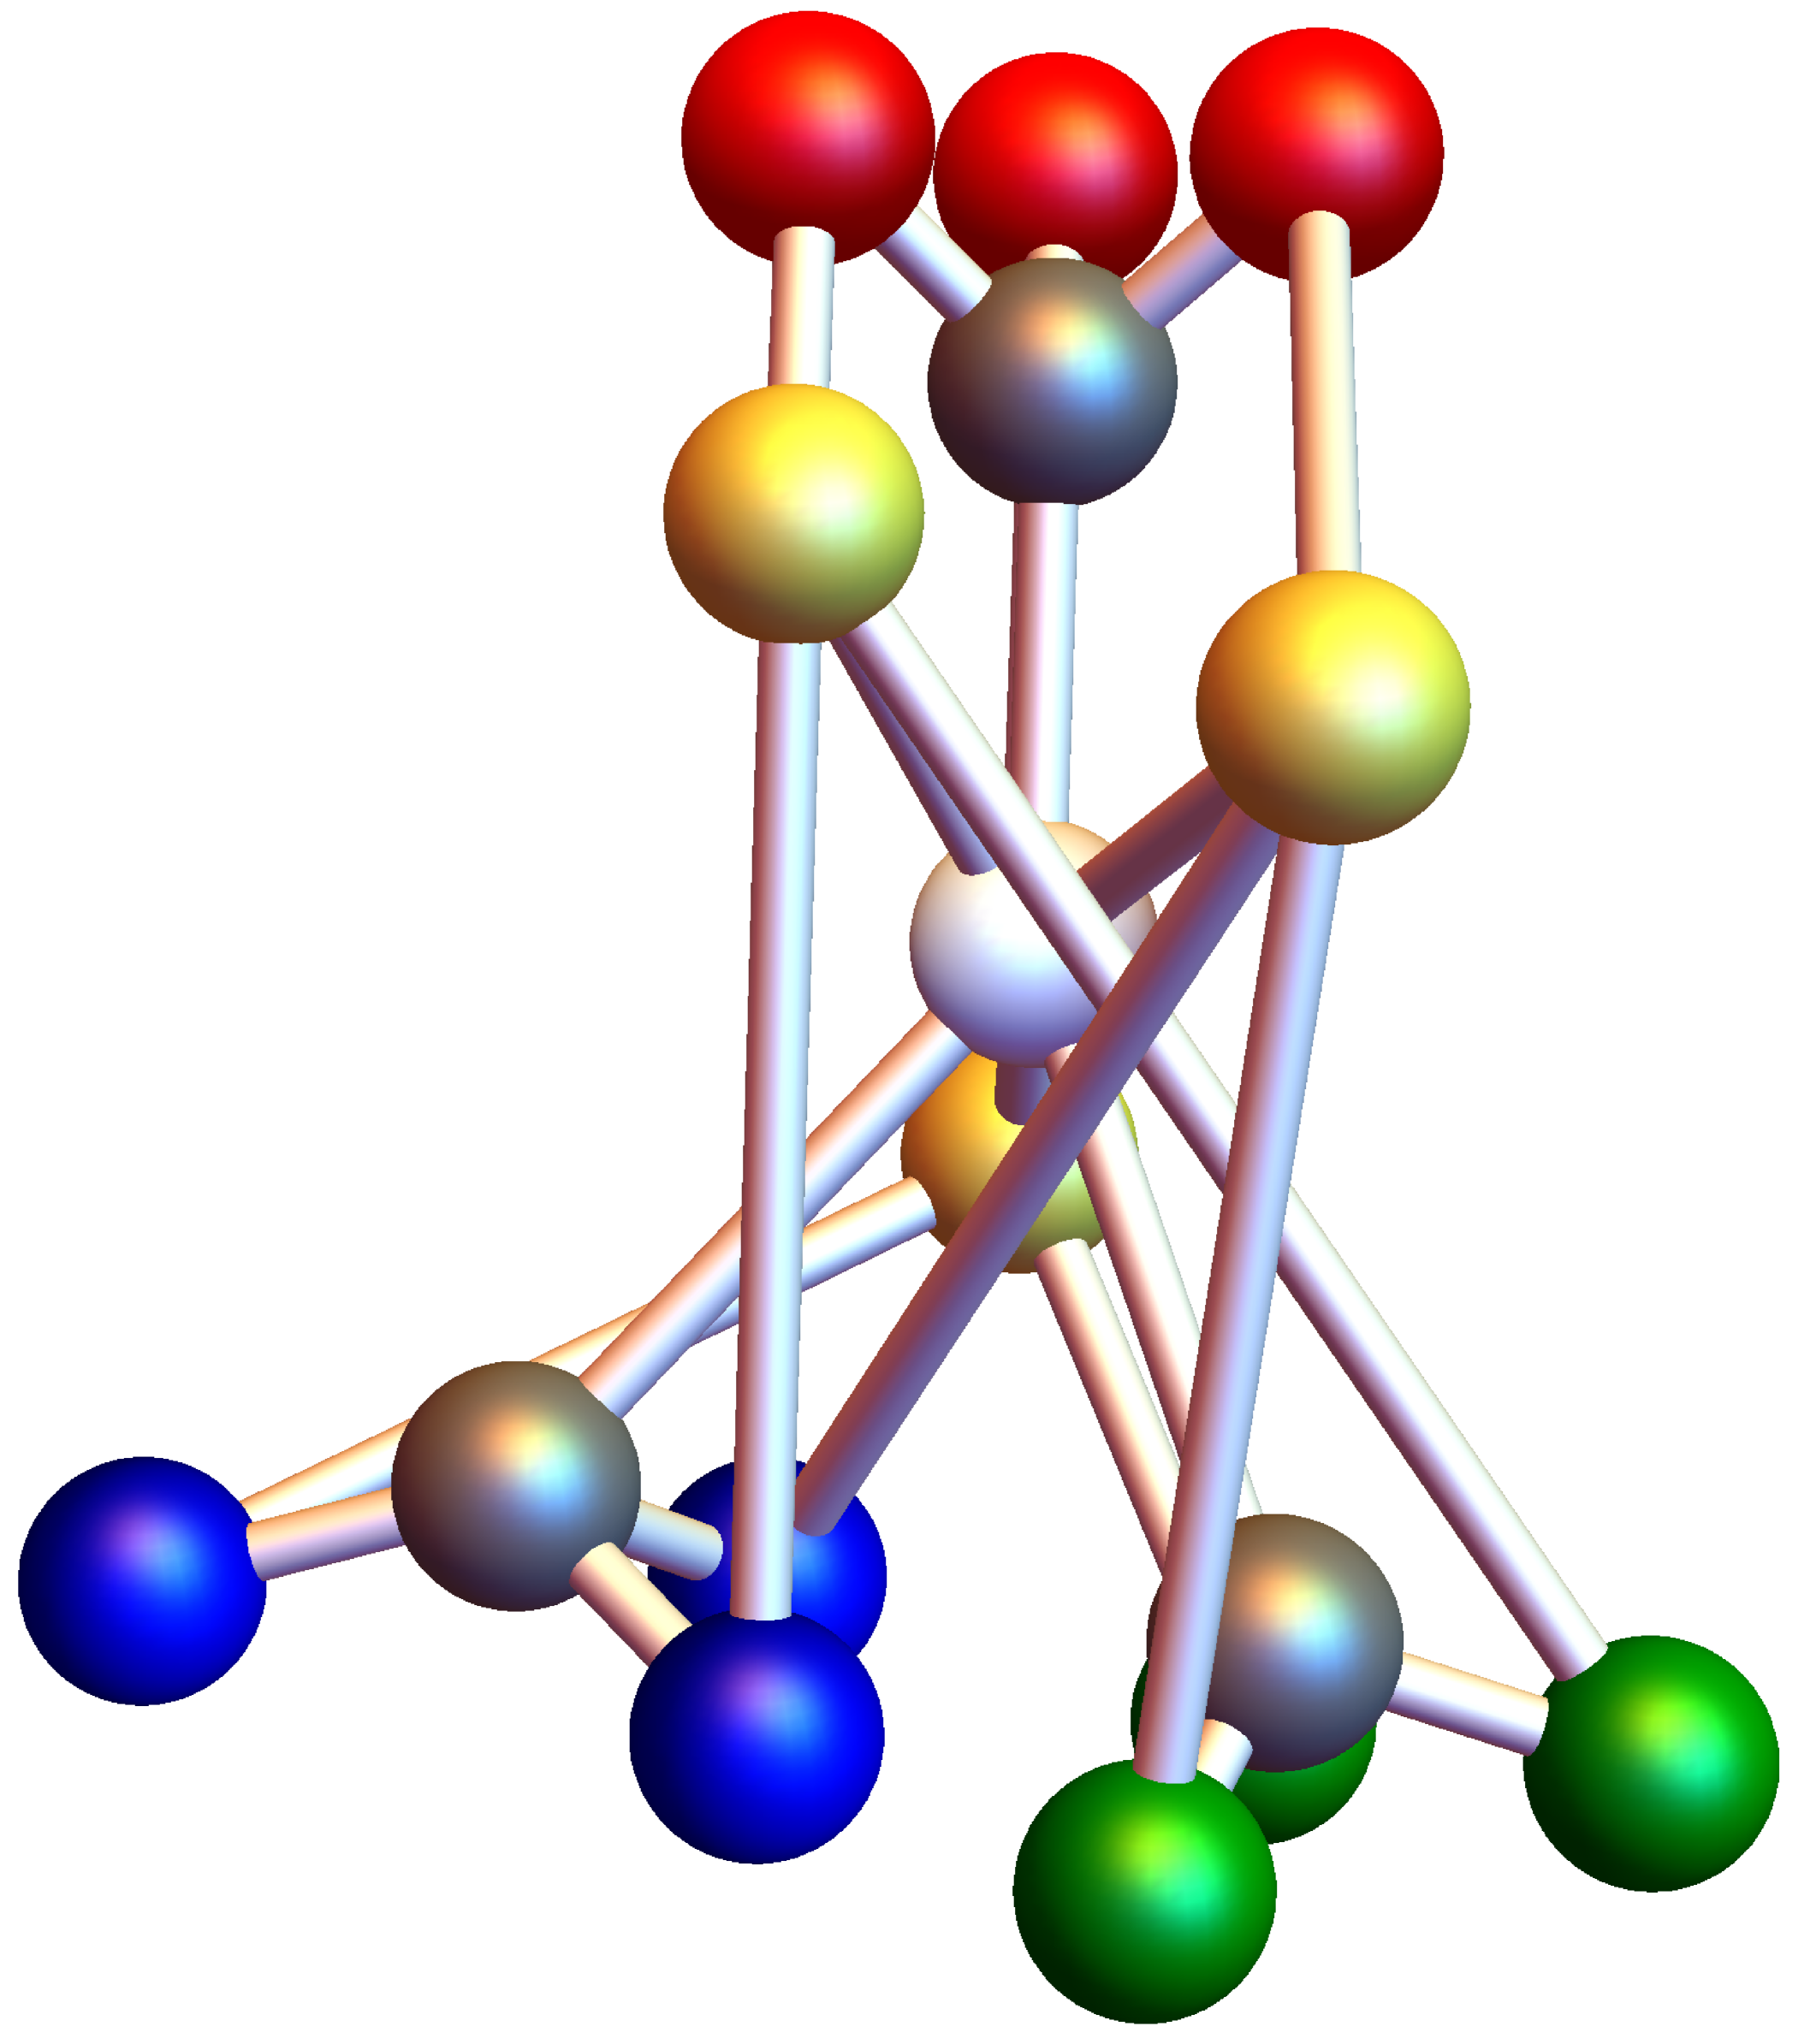
\includegraphics[trim=0 0 0 18mm, width=0.6\textwidth]{Images/switch_square}
		\end{column}
	\end{columns}
\end{frame}}

\begin{center}
	\includeslide{entanglement}
\end{center}

\noindent text

\mode<presentation>{\begin{frame}{Result Extraction}\label{extraction}
	\begin{columns}[T]
		\begin{column}{0.33\textwidth}
			\centering
   			6-qubit ring
   			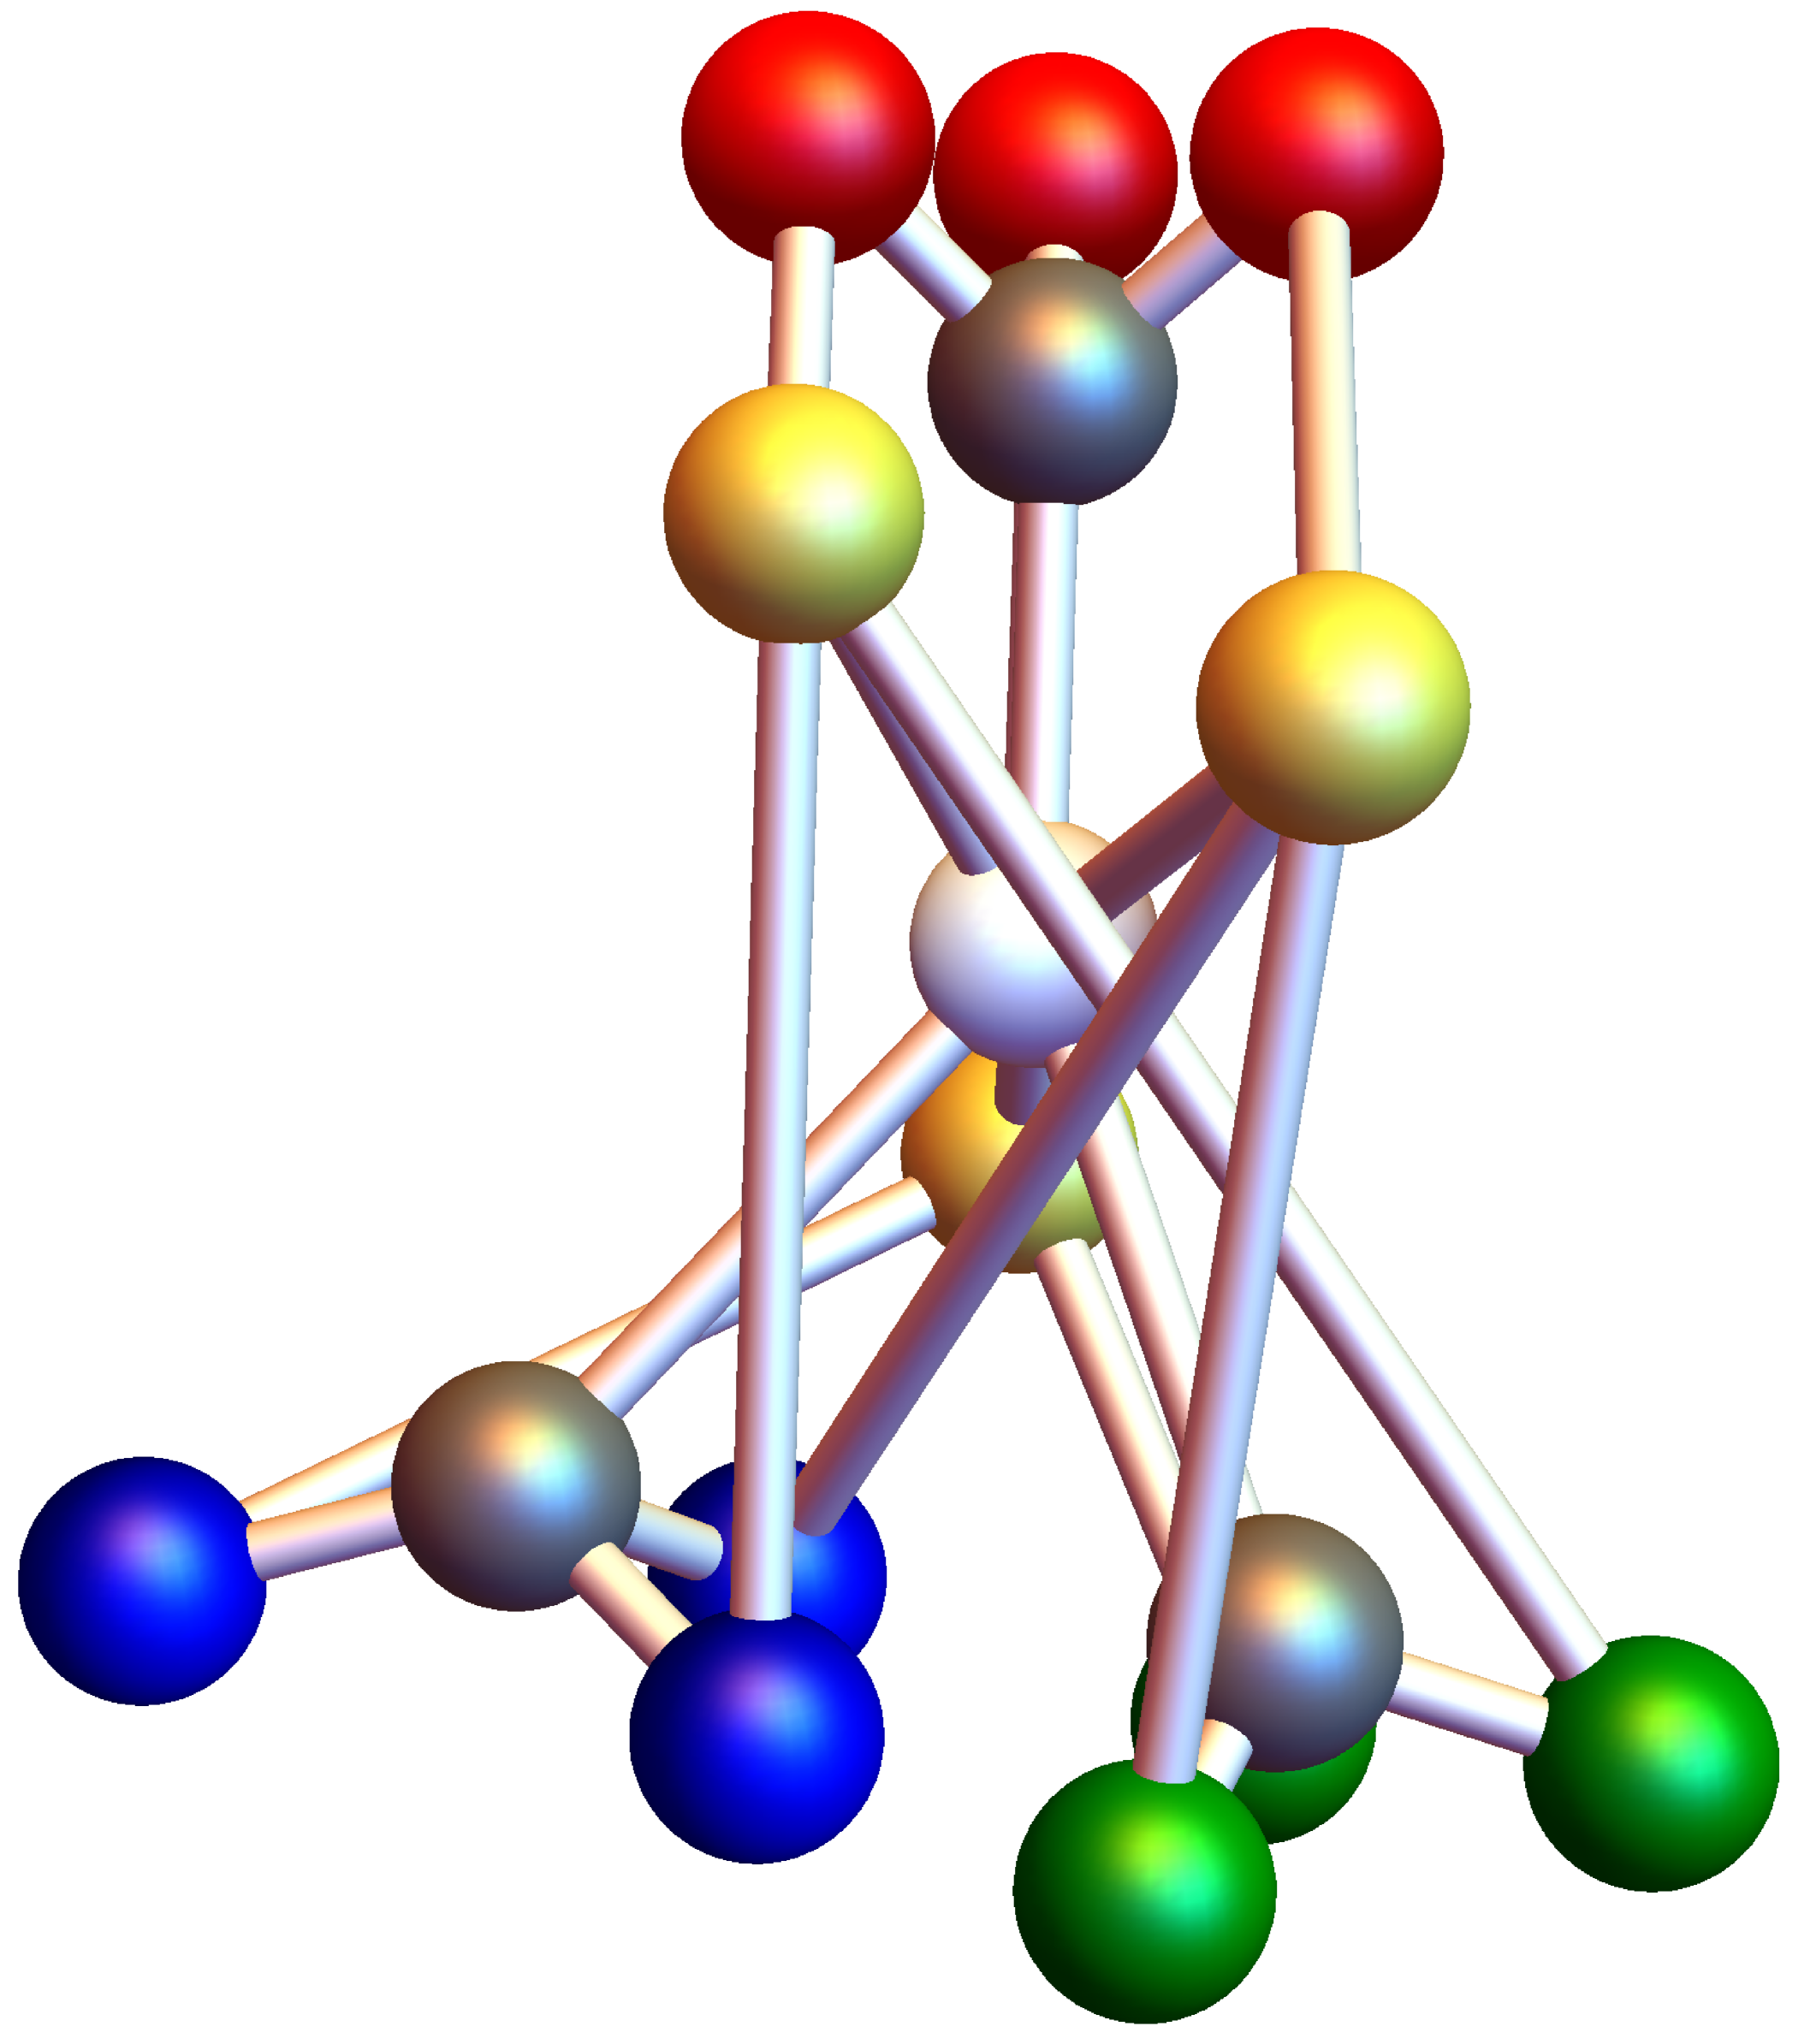
\includegraphics[width=\textwidth]{Images/switch_square}
		\end{column}
		\uncover<2->{\begin{column}{0.33\textwidth}
			\centering
    		Graph
    		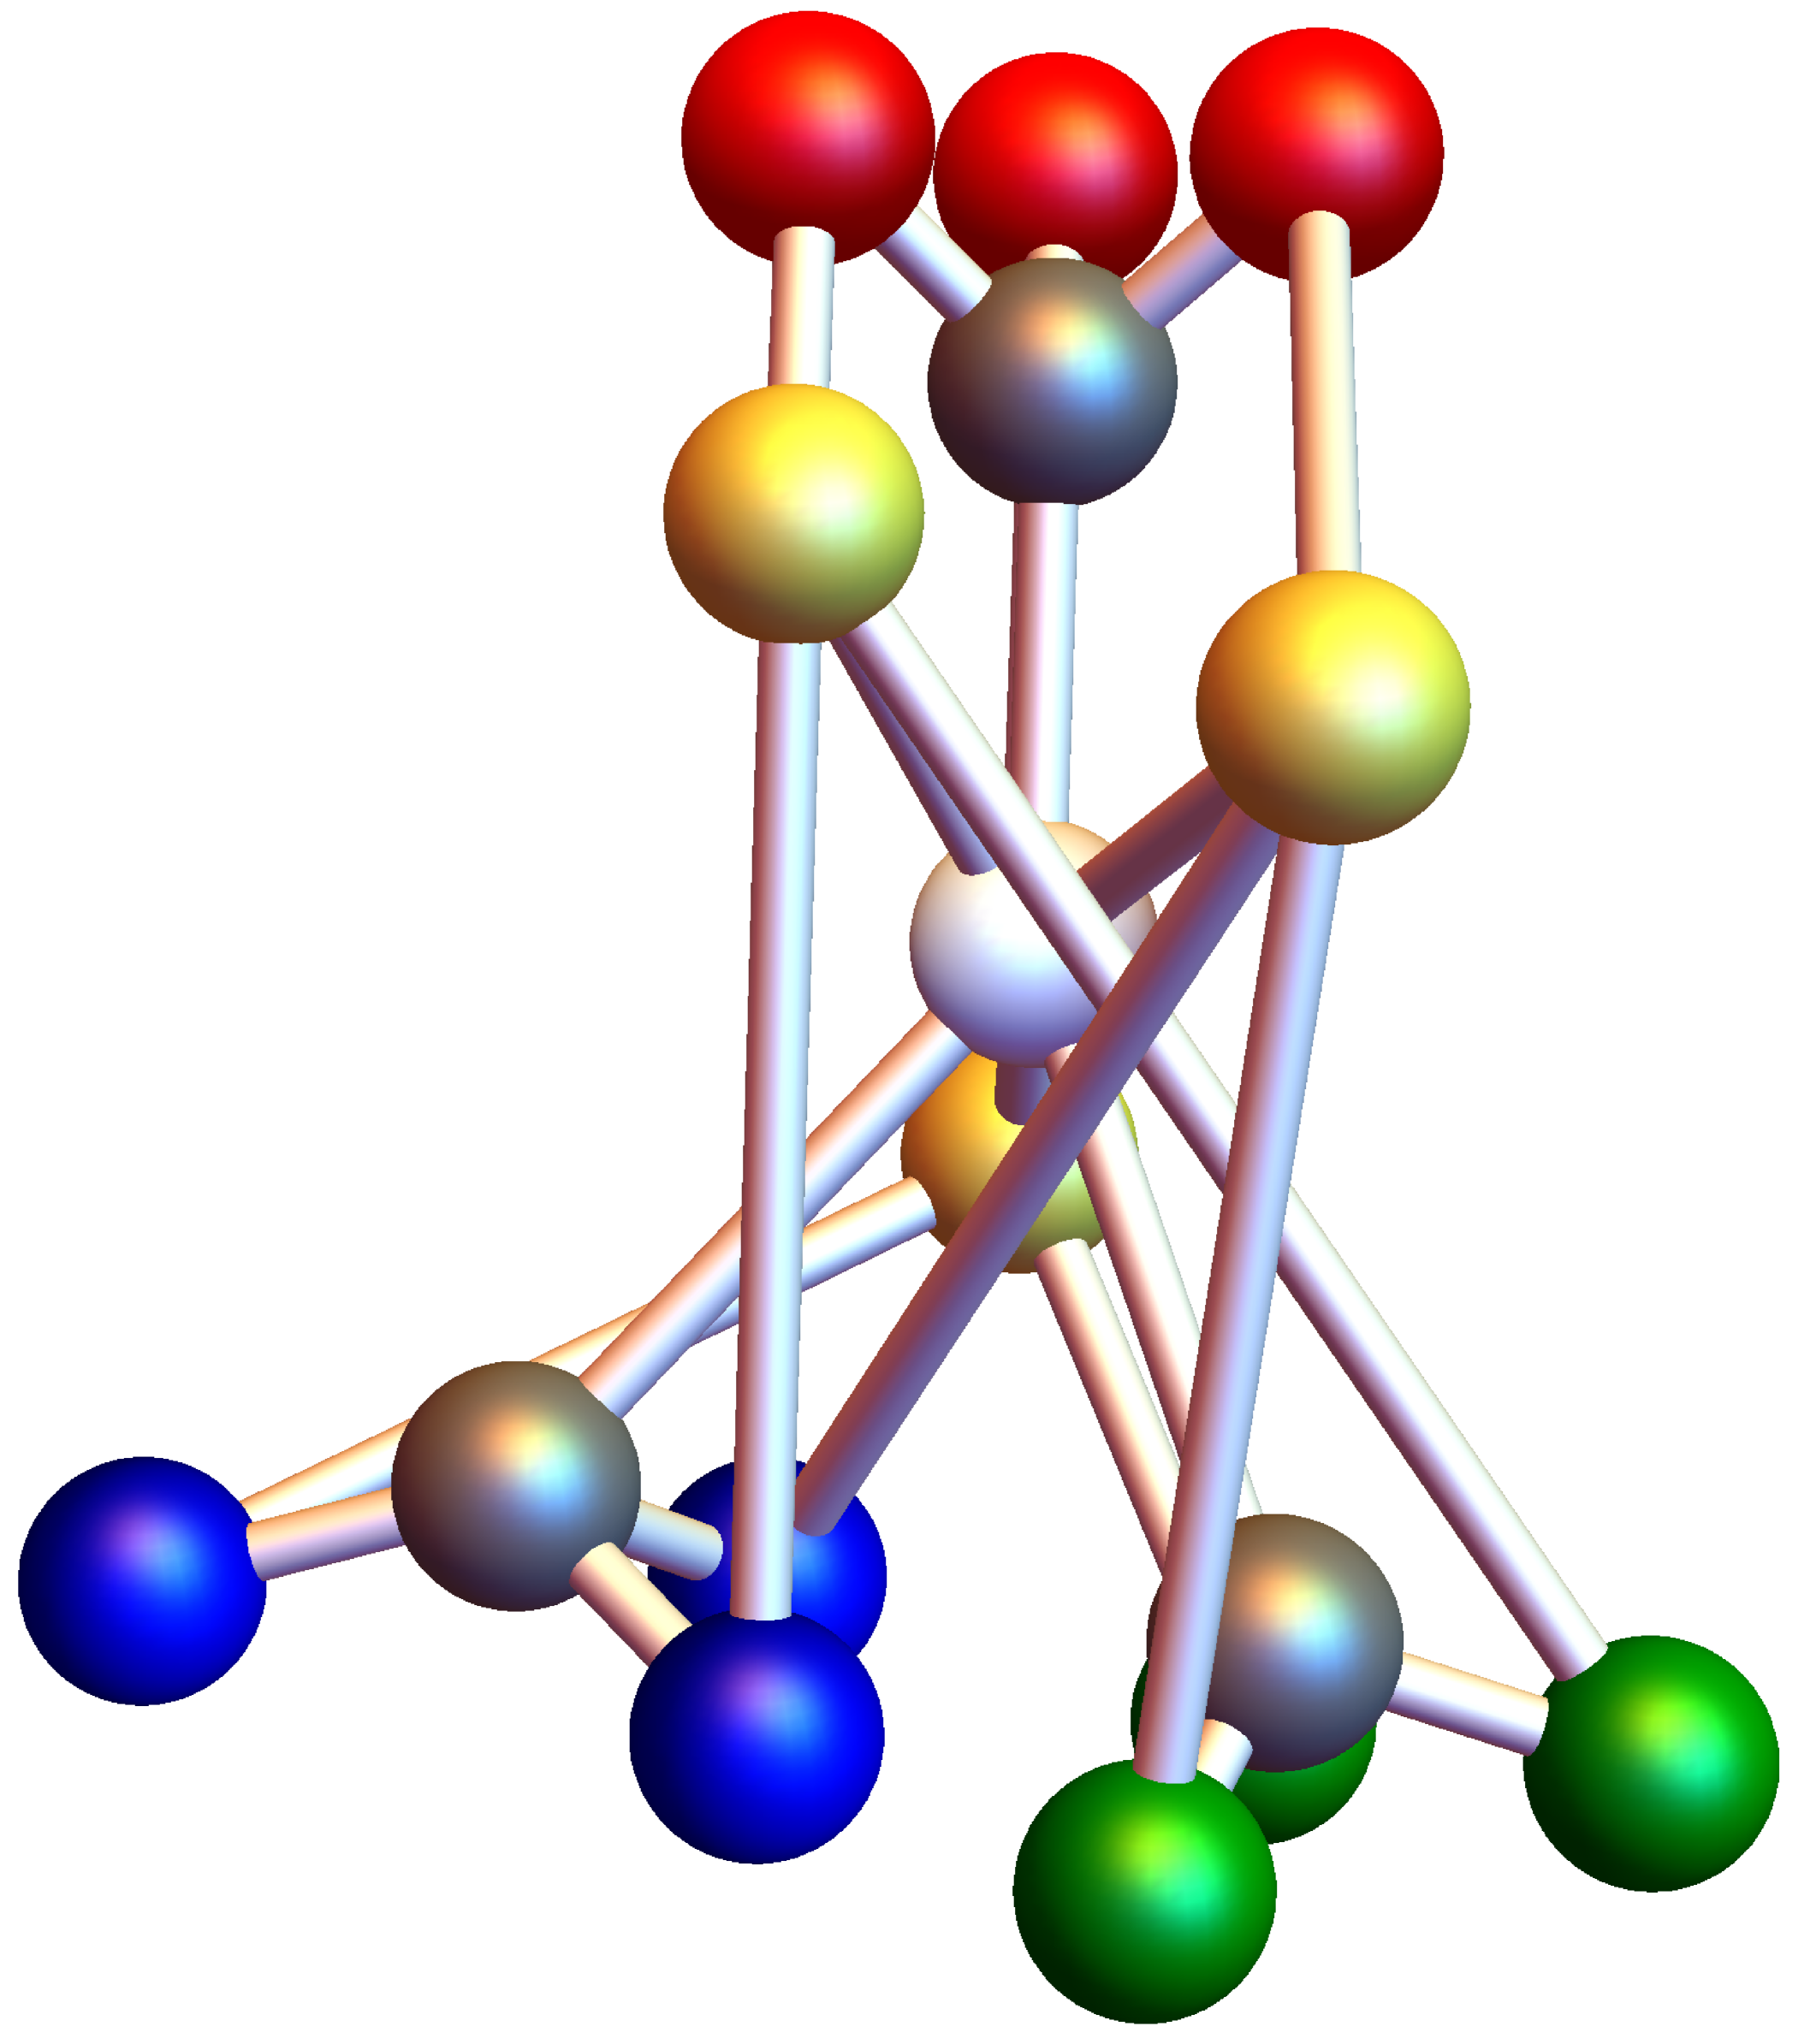
\includegraphics[trim=0 0 0 0mm, width=\textwidth]{Images/switch_square}
		\end{column}}
     	\uncover<3->{\begin{column}{0.33\textwidth}
     		\centering
     		Single spin subspace
     		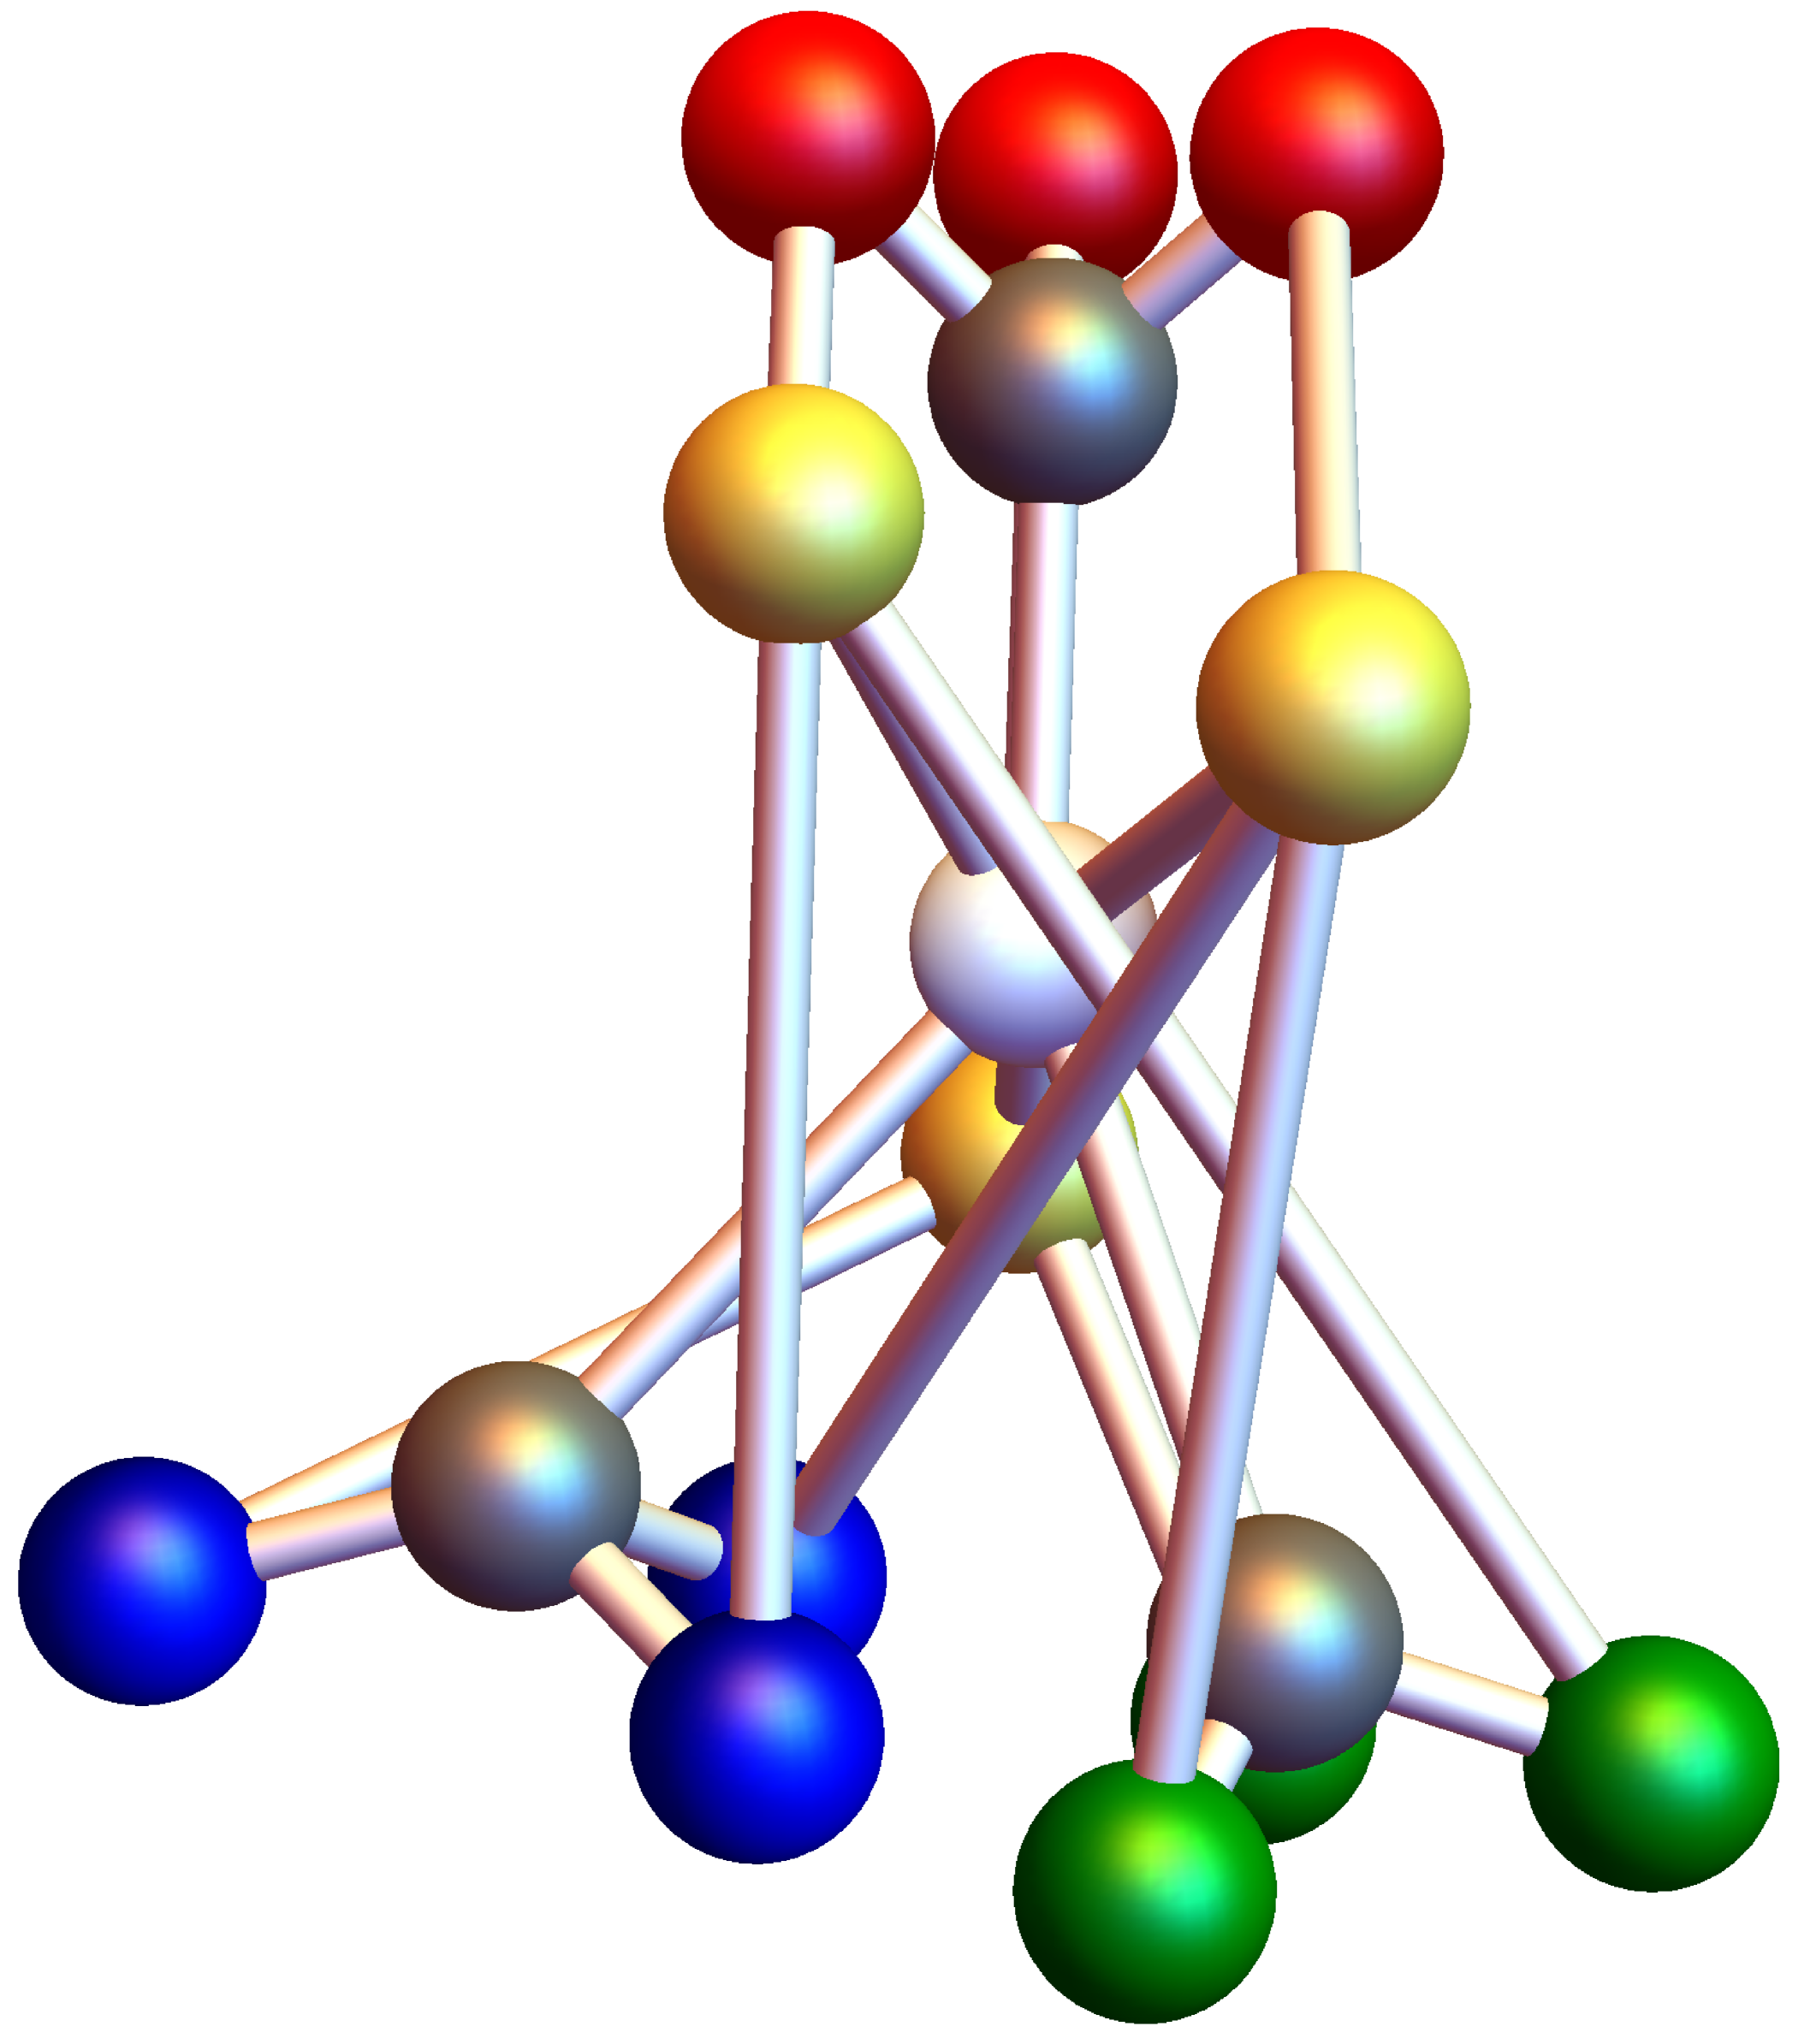
\includegraphics[trim=0 0 0 0mm, width=\textwidth]{Images/switch_square}\\
     		\uncover<4->{This is the adjacency matrix for the 6-qubit ring!}
		\end{column}}
	\end{columns}
\end{frame}}

\begin{center}
	\includeslide{extraction}
\end{center}

\noindent text

\subsection{Techniques}

\mode<presentation>{\begin{frame}[t]{Amplitude Amplification}\label{amplification}
	\begin{exampleblock}{}
	\setlength\abovedisplayskip{-8pt}
	\begin{center}
		$G \times H = (V_{G\times H},E_{G\times H})$
	\end{center}
	\end{exampleblock}
	\begin{itemize}
		\item $V_{G\times H} = V(G) \times V(H)$
		\item $\{(u,u'),(v,v')\} \in E_{G\times H}$ if 
		\begin{itemize}
			\item $u = v$ and $\{u',v'\} \in E_H$ or
			\item $u' = v'$ and $\{u,v\} \in E_G$
		\end{itemize}
	\end{itemize}
	\begin{exampleblock}{}
	\setlength\abovedisplayskip{-8pt}
	\begin{center}
		$A_{G\times H} = A_G \otimes \text{1}_{\left|V_H\right|} + \text{1}_{\left|V_G\right|} \otimes A_H$
	\end{center}
	\end{exampleblock}
\end{frame}}

\begin{center}
	\includeslide{amplification}
\end{center}

\noindent text

\mode<presentation>{\begin{frame}{Quantum Fourier Transformation}\label{QFT}
	\begin{align*}
		f^{\left|V_{G\times H}\right|}_{(r,r'),(s,s')}(t) &= \left( \bra{r} \otimes \bra{r'} \right)e^{-\text{i}A_{G\times H}t} \left( \ket{s} \otimes \ket{s'} \right) \\
		&= \left( \bra{r} \otimes \bra{r'} \right)e^{-\text{i}(A_G \otimes \text{1}_{\left|V_H\right|})t} e^{-\text{i}(\text{1}_{\left|V_G\right|} \otimes A_H)t} \left( \ket{s} \otimes \ket{s'} \right) \\
		&= \sum_{k=1}^{K}\left[ \left( \bra{r} \otimes \bra{r'} \right) \ket{g'_k}\bra{g'_k}e^{-\text{i}G_k{}'t} \ket{h_k'}\bra{h_k'}e^{-\text{i}H_k{}'t} \left( \ket{s} \otimes \ket{s'} \right) \right]
	\end{align*}
	\begin{itemize}
		\item $K = \left|V_{G\times H}\right|$, $L = \left|V_G\right|$, $M = \left|V_H\right| \rightarrow K = L\cdot M$
		\item $\bra{g'_k} = \bra{g_l} \otimes \bra{e_m}$, $\bra{h'_k} = \bra{e_l} \otimes \bra{h_m}$ etc.
		\item $G_k{}' = G_l\cdot E_m$, $H_k{}' = E_l\cdot H_m$
		\item $(A\otimes B)(C\otimes D) = (AC)\otimes (BD)$
	\end{itemize}
	\begin{align*}
		f^{\left|V_{G\times H}\right|}_{(r,r'),(s,s')}(t) &= \sum_{l=1}^L\left[ \Braket{r|g_l}\Braket{g_l|s}e^{-\text{i}G_l t} \right] \sum_{m=1}^M\left[ \Braket{r'|h_m}\Braket{h_m|s'}e^{-\text{i}H_mt} \right] \\
		&= \Braket{r|e^{-\text{i}A_G t}|s}\Braket{r'|e^{-\text{i}A_H t}|s'}
	\end{align*}
\end{frame}}

\begin{center}
	\includeslide{QFT}
\end{center}

\noindent text


\mode<presentation>{\begin{frame}{Quantum Random Walk}\label{randomwalk}
	\begin{align*}
		f^{\left|V_{G\times H}\right|}_{(r,r'),(s,s')}(t) &= \left( \bra{r} \otimes \bra{r'} \right)e^{-\text{i}A_{G\times H}t} \left( \ket{s} \otimes \ket{s'} \right) \\
		&= \left( \bra{r} \otimes \bra{r'} \right)e^{-\text{i}(A_G \otimes \text{1}_{\left|V_H\right|})t} e^{-\text{i}(\text{1}_{\left|V_G\right|} \otimes A_H)t} \left( \ket{s} \otimes \ket{s'} \right) \\
		&= \sum_{k=1}^{K}\left[ \left( \bra{r} \otimes \bra{r'} \right) \ket{g'_k}\bra{g'_k}e^{-\text{i}G_k{}'t} \ket{h_k'}\bra{h_k'}e^{-\text{i}H_k{}'t} \left( \ket{s} \otimes \ket{s'} \right) \right]
	\end{align*}
	\begin{itemize}
		\item $K = \left|V_{G\times H}\right|$, $L = \left|V_G\right|$, $M = \left|V_H\right| \rightarrow K = L\cdot M$
		\item $\bra{g'_k} = \bra{g_l} \otimes \bra{e_m}$, $\bra{h'_k} = \bra{e_l} \otimes \bra{h_m}$ etc.
		\item $G_k{}' = G_l\cdot E_m$, $H_k{}' = E_l\cdot H_m$
		\item $(A\otimes B)(C\otimes D) = (AC)\otimes (BD)$
	\end{itemize}
	\begin{align*}
		f^{\left|V_{G\times H}\right|}_{(r,r'),(s,s')}(t) &= \sum_{l=1}^L\left[ \Braket{r|g_l}\Braket{g_l|s}e^{-\text{i}G_l t} \right] \sum_{m=1}^M\left[ \Braket{r'|h_m}\Braket{h_m|s'}e^{-\text{i}H_mt} \right] \\
		&= \Braket{r|e^{-\text{i}A_G t}|s}\Braket{r'|e^{-\text{i}A_H t}|s'}
	\end{align*}
\end{frame}}

\begin{center}
	\includeslide{randomwalk}
\end{center}

\noindent text


\mode<presentation>{\begin{frame}[t]{QC Strengths}\label{strengths}
	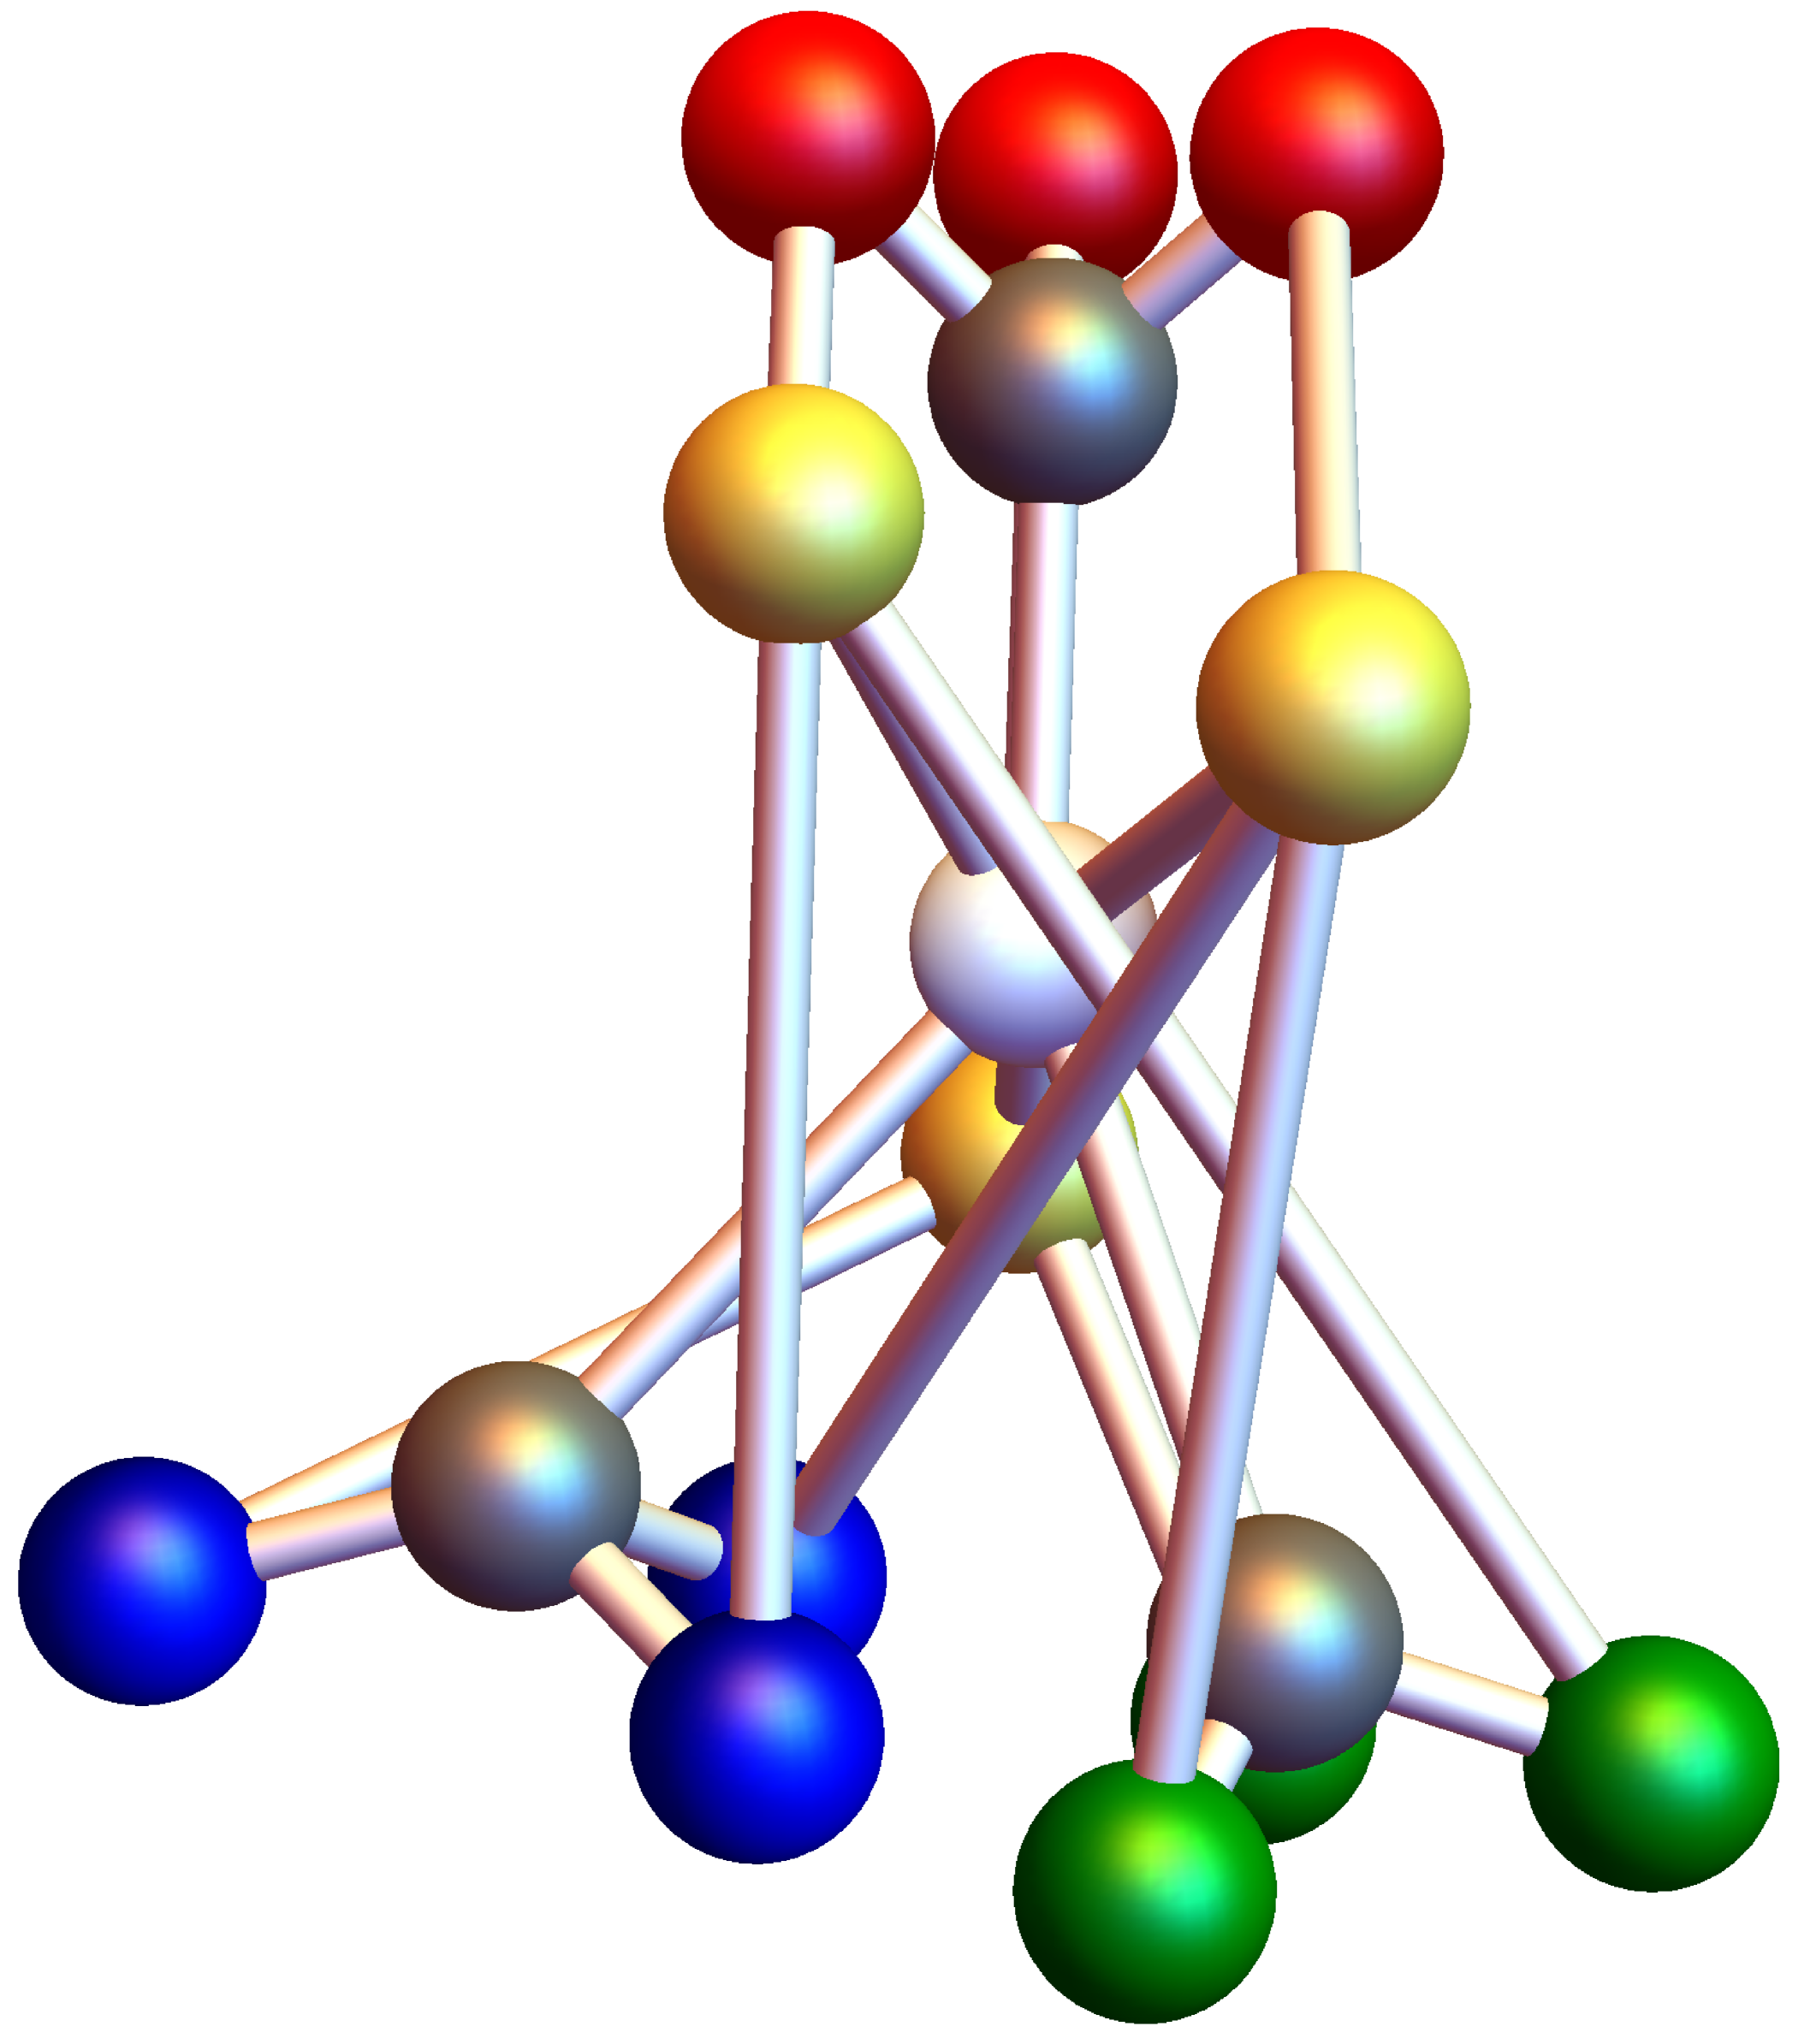
\includegraphics[trim=0 0 0 0, width=\textwidth]{Images/switch_square}\\
	\[f_{N,1}^N(t) = \frac{2}{N+1}\sum_{s}^N\sin\left(\frac{\pi s}{N+1}\right)\sin\left(\frac{\pi sN}{N+1}\right)e^{-\text{i}E_s t} \]
	\begin{itemize}
		\item $N=2$: \,\,\,\,$f_{2,1}^2(t) = -\text{i}\sin(t)$ \,\,\,\,\,\,\,\,\,\,\,\,\,\,\,\,\,with $\tau_2 = \pi/2$
		\item $N=3$: \,\,\,\,$f_{3,1}^3(t) = -\left[\sin(t/\sqrt{2})\right]^2$ with $\tau_3 = \pi/\sqrt{2}$
		\item $N \geq 4$: \,\,\,\,$f_{N,1}^N(t) \neq 1$\,\,\, $\forall$\,\,$t$
	\end{itemize}
	\begin{columns}[T]
		\begin{column}{0.5\textwidth}
			\centering
			\begin{exampleblock}{}
			\setlength\abovedisplayskip{-8pt}
			\begin{center}
		Proof shows that $f_{N,1}^N(t) = 1$ implies $\frac{\cos\left(\frac{2\pi}{N+1}\right)}{\cos\left(\frac{\pi}{N+1}\right)} \in \mathbb{Q}$
			\end{center}
			\end{exampleblock}
		\end{column}
		\begin{column}{0.5\textwidth}
			\centering
        $H = \begin{pmatrix}
			0 & 1 & 0 & 0 & 0 \\
			1 & 0 & 1 & 0 & 0 \\
			0 & 1 & 0 & ... & 0 \\
			0 & 0 & ... & 0 & 1 \\
			0 & 0 & 0 & 1 & 0 
		\end{pmatrix}$
		\end{column}
	\end{columns}
\end{frame}}


\begin{center}
	\includeslide{strengths}
\end{center}

\noindent text

\mode<presentation>{\begin{frame}[t]{D-Wave 2x}\label{dwave}
	\begin{exampleblock}{}
	\setlength\abovedisplayskip{-8pt}
	\begin{center}
		\[ H = \frac{1}{2}J\sum_{i=2}^{N}\left[\sigma_1^x\sigma_i^x + \sigma_1^y\sigma_i^y\right] + \sum_{i=1}^{N}h_i\sigma_i^z \]
	\end{center}
	\end{exampleblock}
	\begin{columns}[T]
		\begin{column}{0.5\textwidth}
			\centering
   			\begin{itemize}
				\item Introduce local potentials
				\item Slight variations only
				\item Diagonal entries 
				\item E.g. magnetic offset field
			\end{itemize}
		\end{column}
		\begin{column}{0.5\textwidth}
			\centering
    		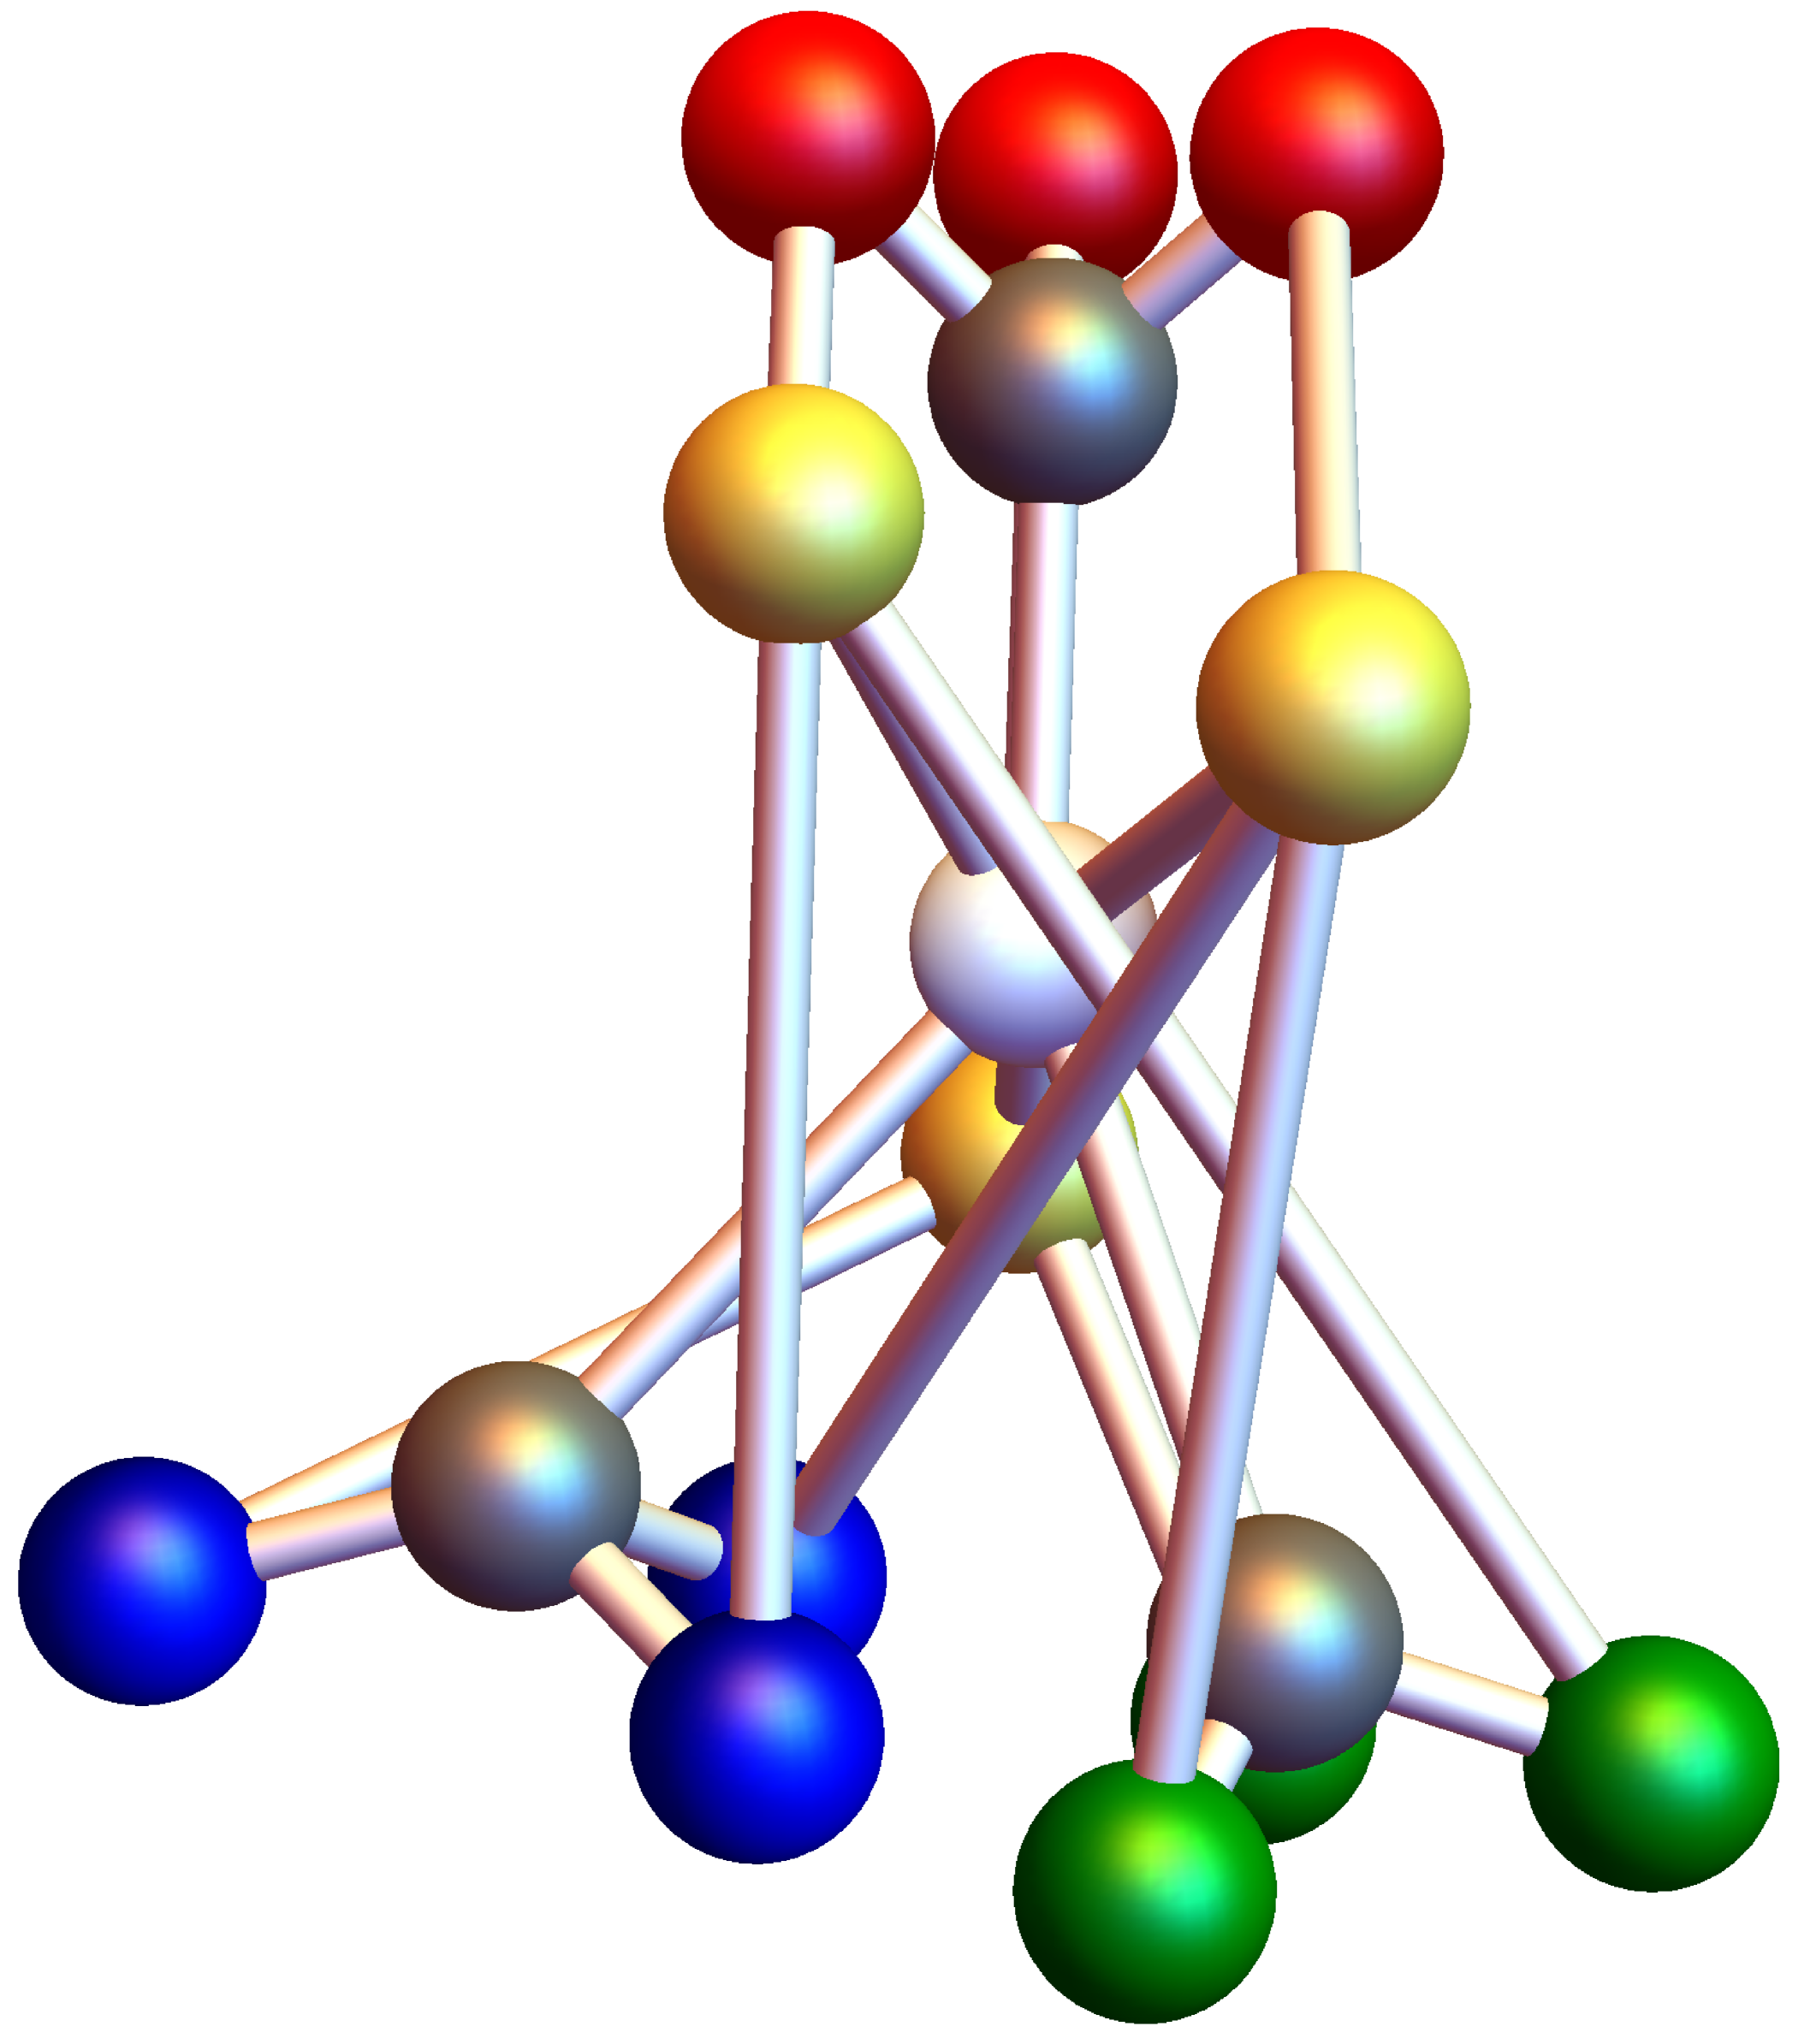
\includegraphics[trim=0mm 0 0 0mm, width=0.8\textwidth]{Images/switch_square}
		\end{column}
	\end{columns}
\end{frame}}


\begin{center}
	\includeslide{dwave}
\end{center}

\noindent text


\mode<presentation>{\begin{frame}{Universal QC}\label{uniqc}
	\begin{columns}[T]
		\begin{column}{0.5\textwidth}
			\centering
   			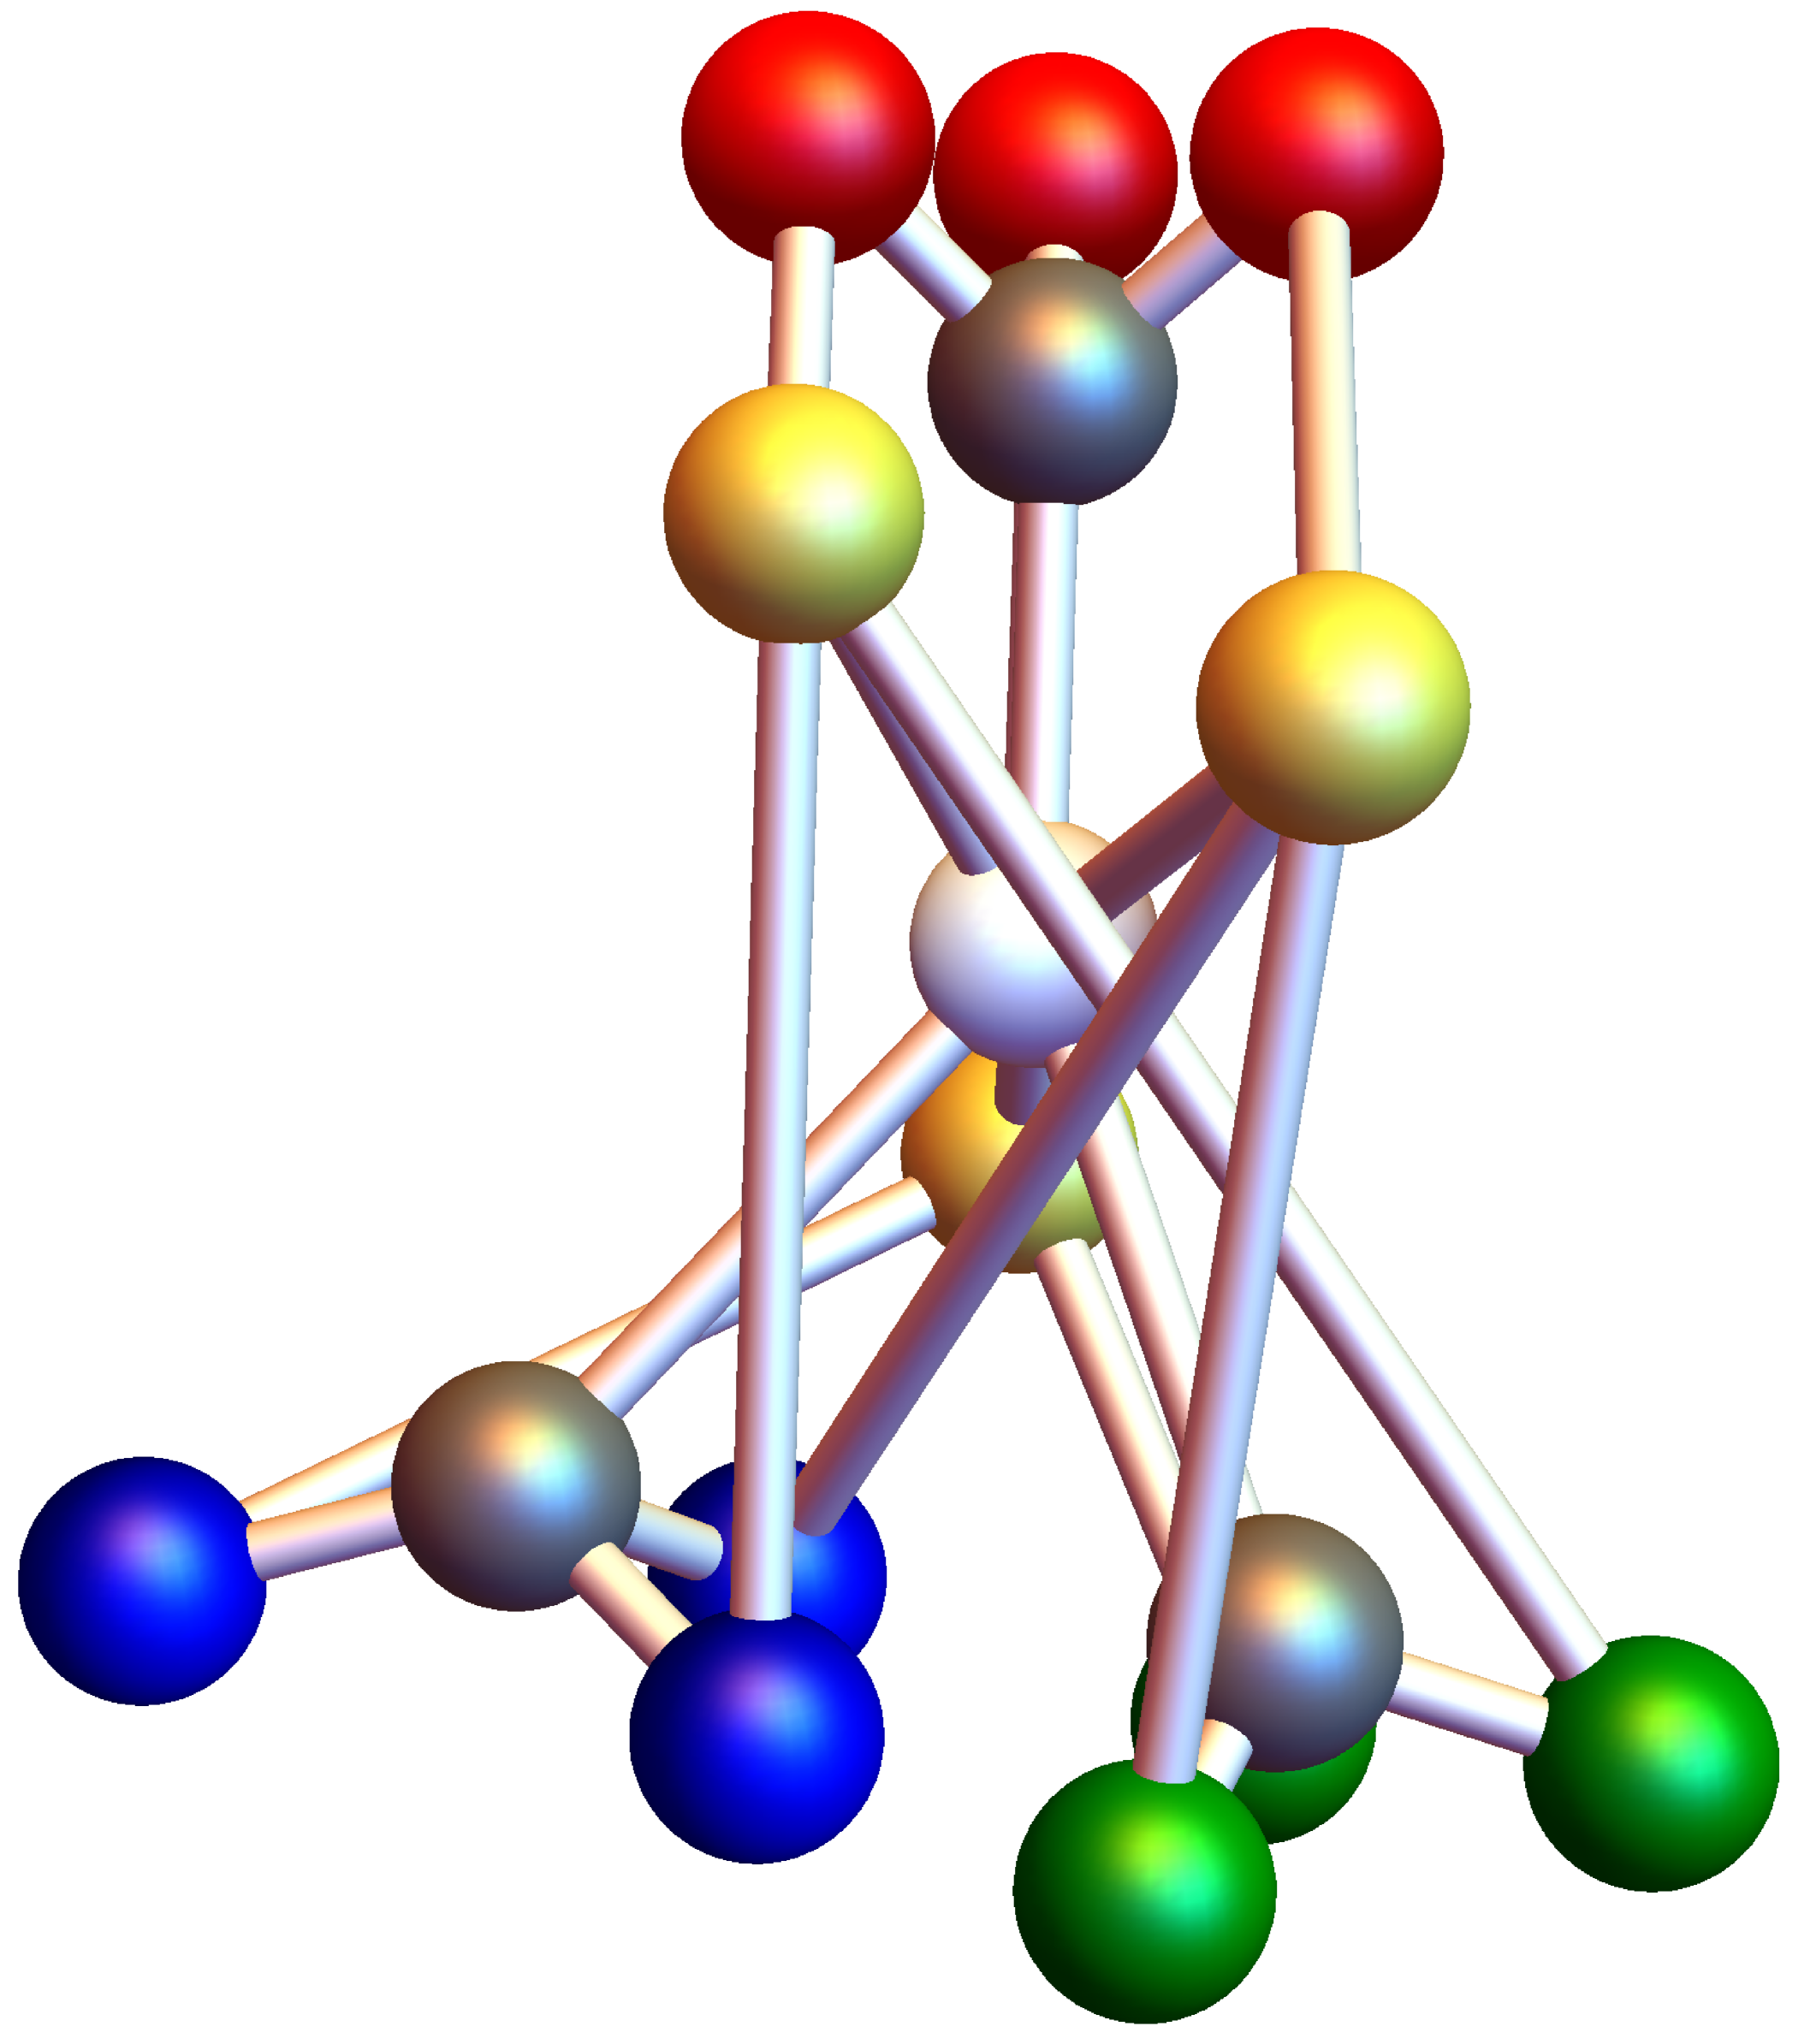
\includegraphics[trim=0mm 0 0 0mm, width=1.2\textwidth]{Images/switch_square}
		\end{column}
		\begin{column}{0.5\textwidth}
			\centering
    		\begin{itemize}
    			\item $h_{u,v} = h_u + h_v \rightarrow $ local potentials are added
    			\item State at vertex $(2,2)$ is transferred to vertex $(3,3)$ or $(4,4)$ at $t = \frac{\pi}{h_2}$
    			\item Symmetry of simple switch $\rightarrow$ transfer from $(2,3)$ to $(3,2)$ or $(2,4)$ to $(4,2)$ with same configuration
    			\item Higher products similar
    		\end{itemize}
		\end{column}
	\end{columns}
\end{frame}}

\begin{center}
	\includeslide{uniqc}
\end{center}

\noindent text

\section{Spin Networks}

\mode<presentation>{\begin{frame}[t]{QC Architecture}\label{architecture}
	\begin{exampleblock}{}
	\setlength\abovedisplayskip{-8pt}
	\begin{center}
		\[H_{XX}=\frac{1}{2}\sum_{i=1}^{N}{J_i\left[\sigma_i^x\sigma_{i+1}^x + \sigma_i^y\sigma_{i+1}^y\right]}\]
	\end{center}
	\end{exampleblock}
	\begin{columns}[T]
		\begin{column}{0.5\textwidth}
			\centering
			Weighted graphs
   			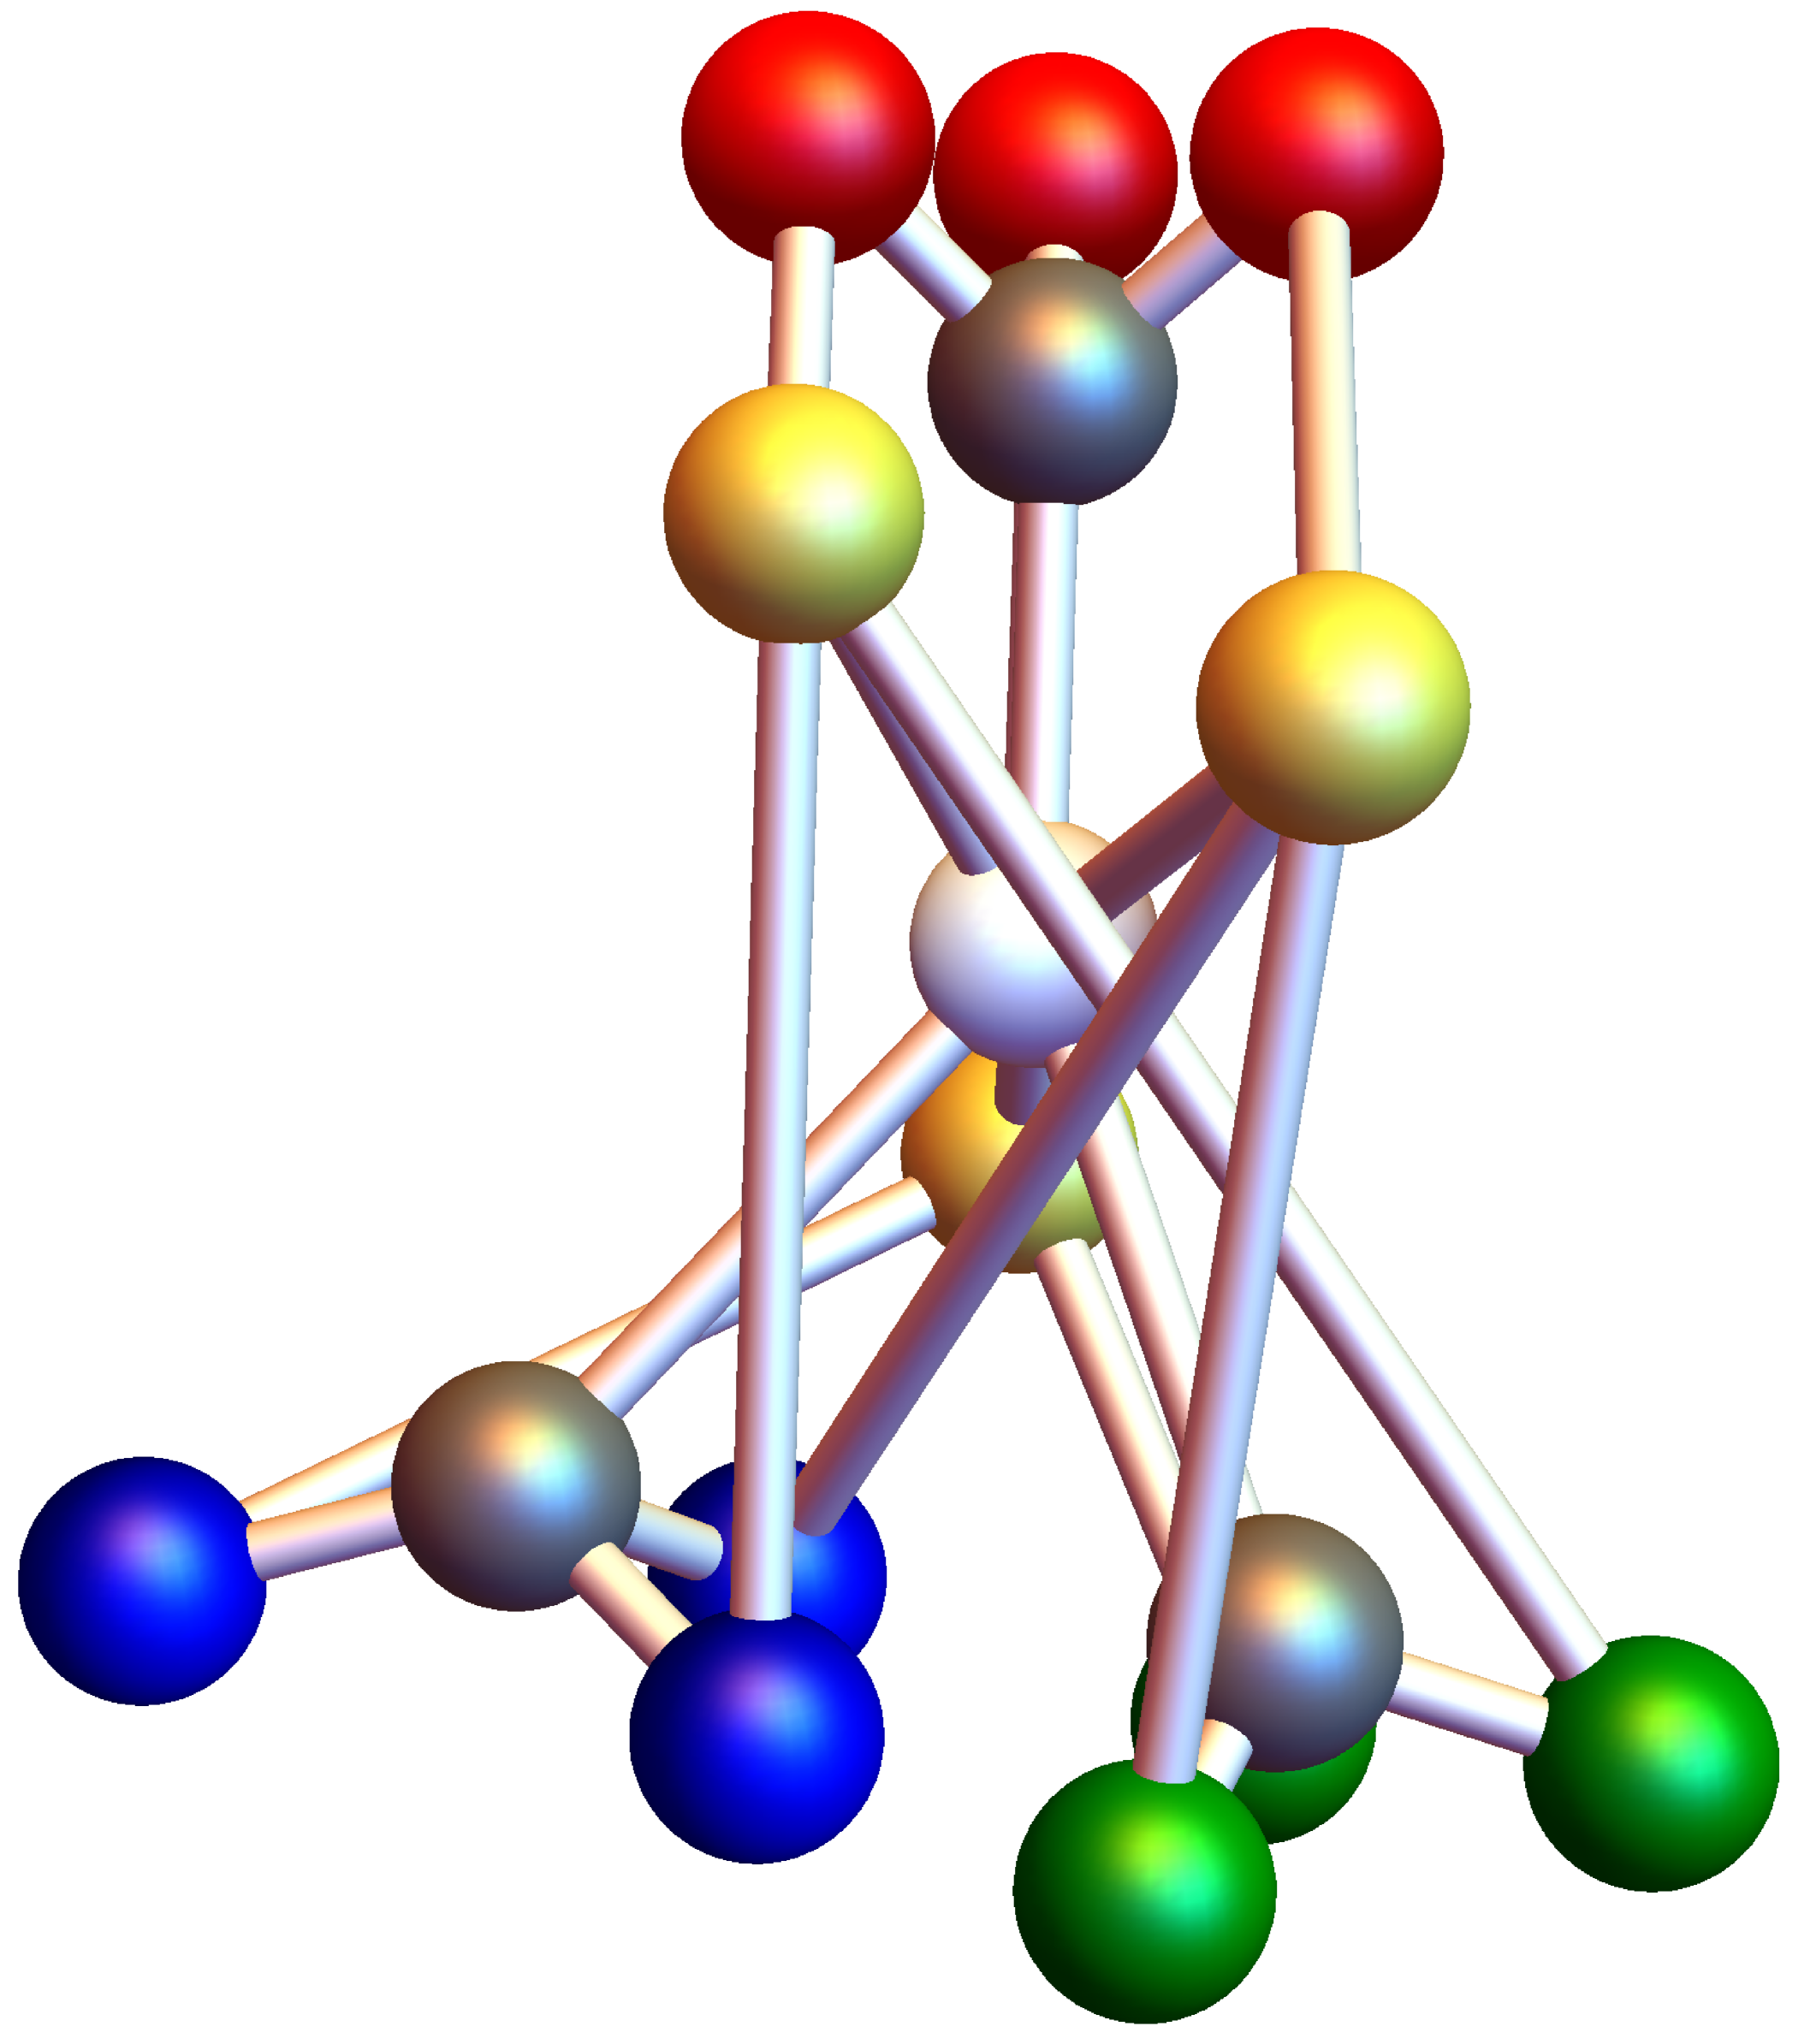
\includegraphics[trim=0mm 0 0 0mm, width=0.8\textwidth]{Images/switch_square}
		\end{column}
		\begin{column}{0.5\textwidth}
			\centering
			Weighted adjacency matrices
   			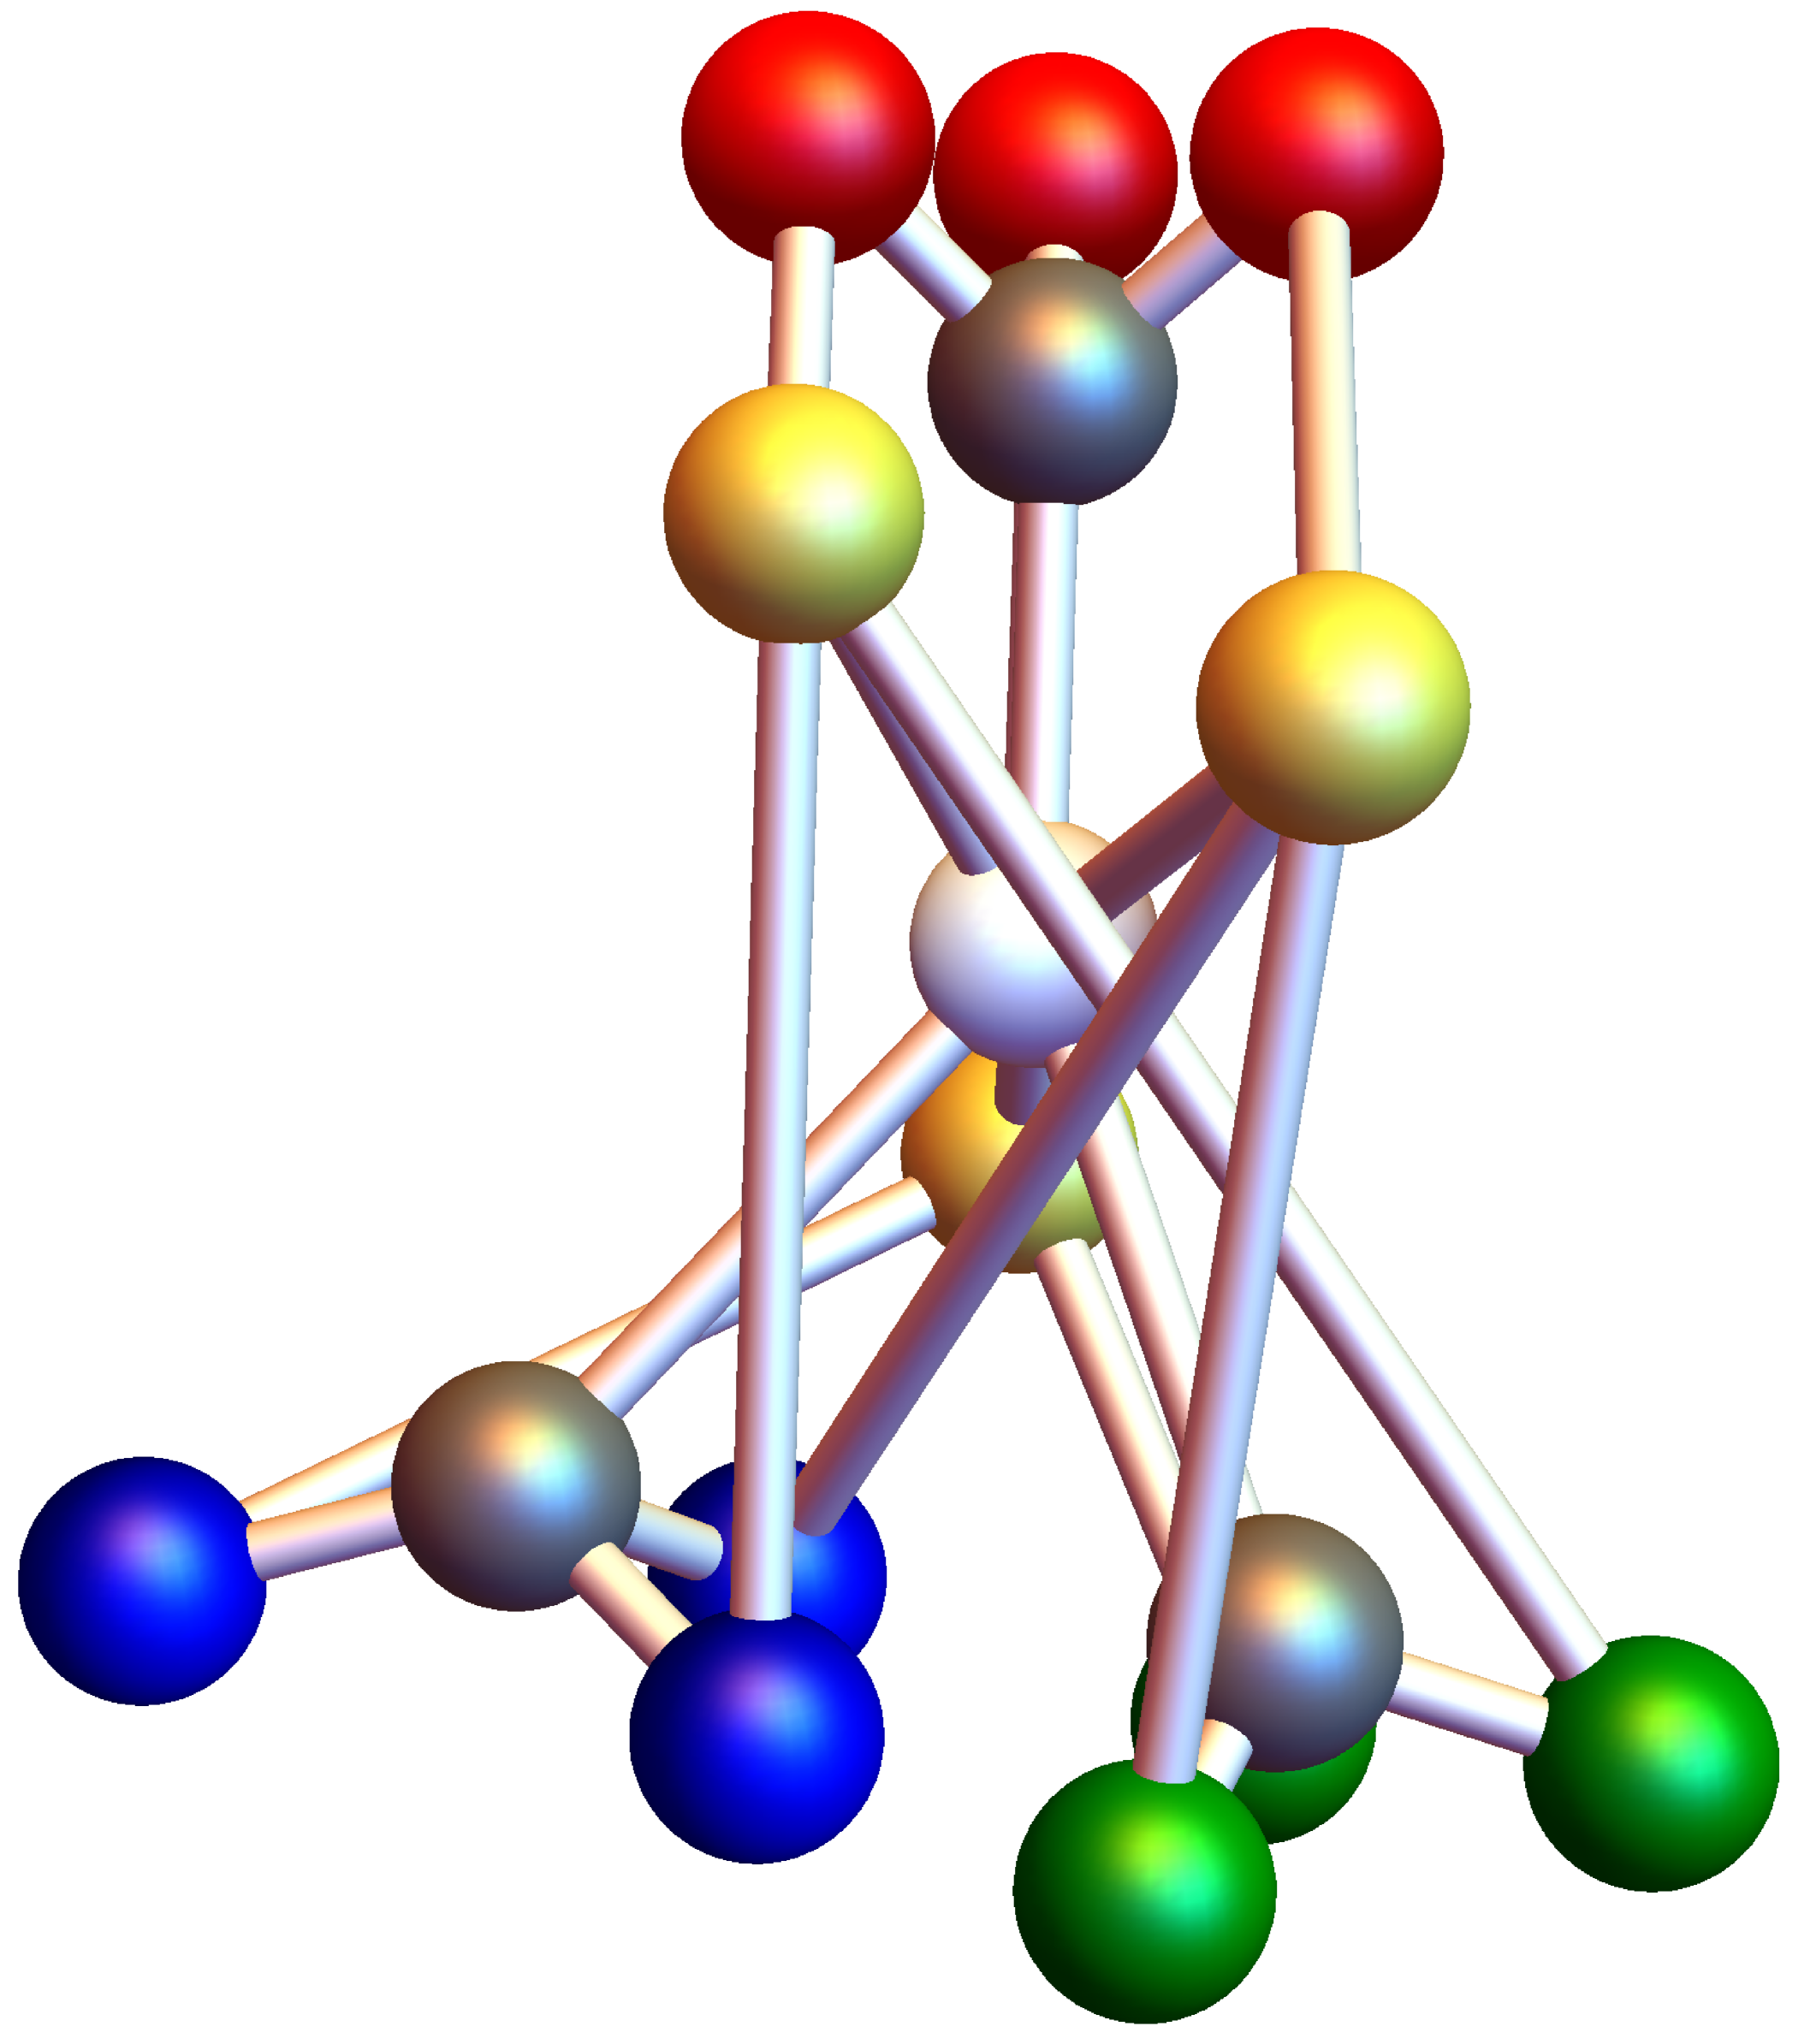
\includegraphics[trim=0mm 0 0 0mm, width=0.7\textwidth]{Images/switch_square}
		\end{column}
	\end{columns}
\end{frame}}


\begin{center}
	\includeslide{architecture}
\end{center}

\noindent text


\mode<presentation>{\begin{frame}{Setup}\label{setup} %[fragile,t] for listings
	\begin{columns}
		\begin{column}{0.5\textwidth}
			\centering
				\begin{itemize}
		\item PST in larger networks
		\item Control more than one qubit
		\begin{itemize}
			\item Quantum error correction and fault tolerance
		\end{itemize}
		\item Prepare multiple states, send to different target sites
	\end{itemize}
		\end{column}
		\begin{column}{0.5\textwidth}
			\centering
			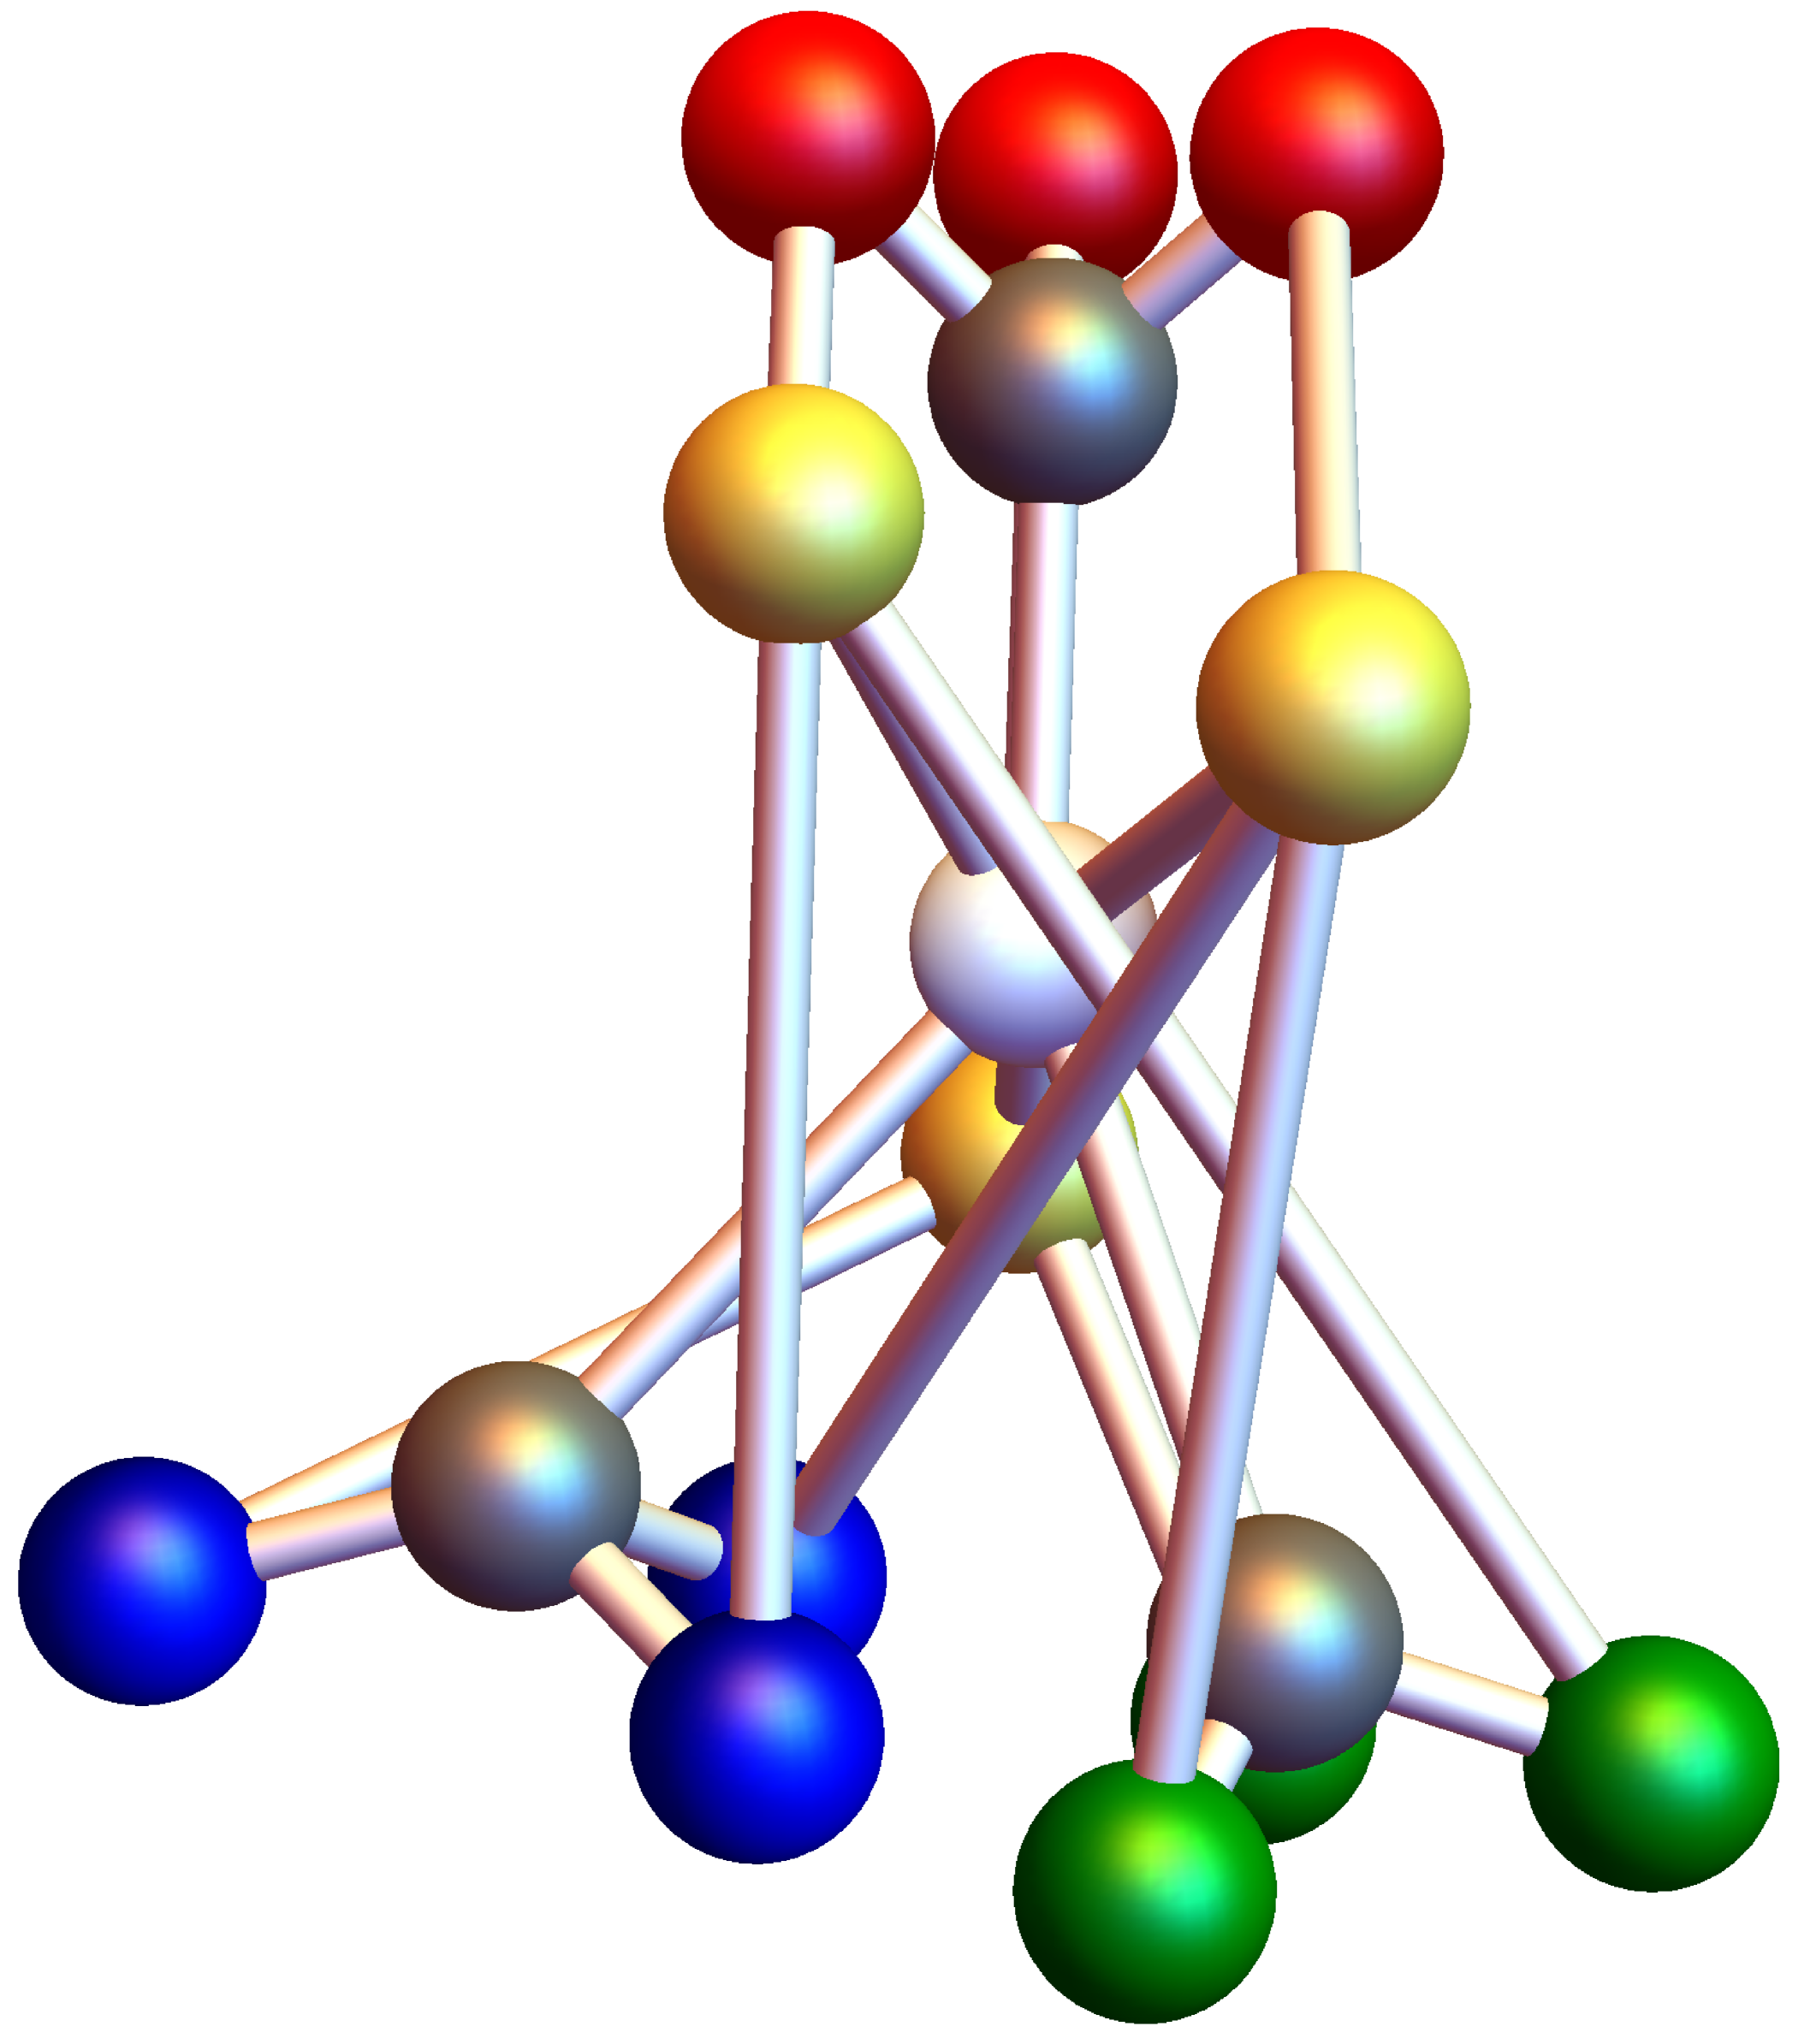
\includegraphics[trim=0mm 0 0 0mm, width=\textwidth]{Images/switch_square}\\
			Calculating higher spin graphs from single spin graphs is an easy task.
		\end{column}
	\end{columns}
\end{frame}}

\begin{center}
	\includeslide{setup}
\end{center}

\noindent text


\mode<presentation>{\begin{frame}{Graphs}\label{graphs}
	\begin{center}
		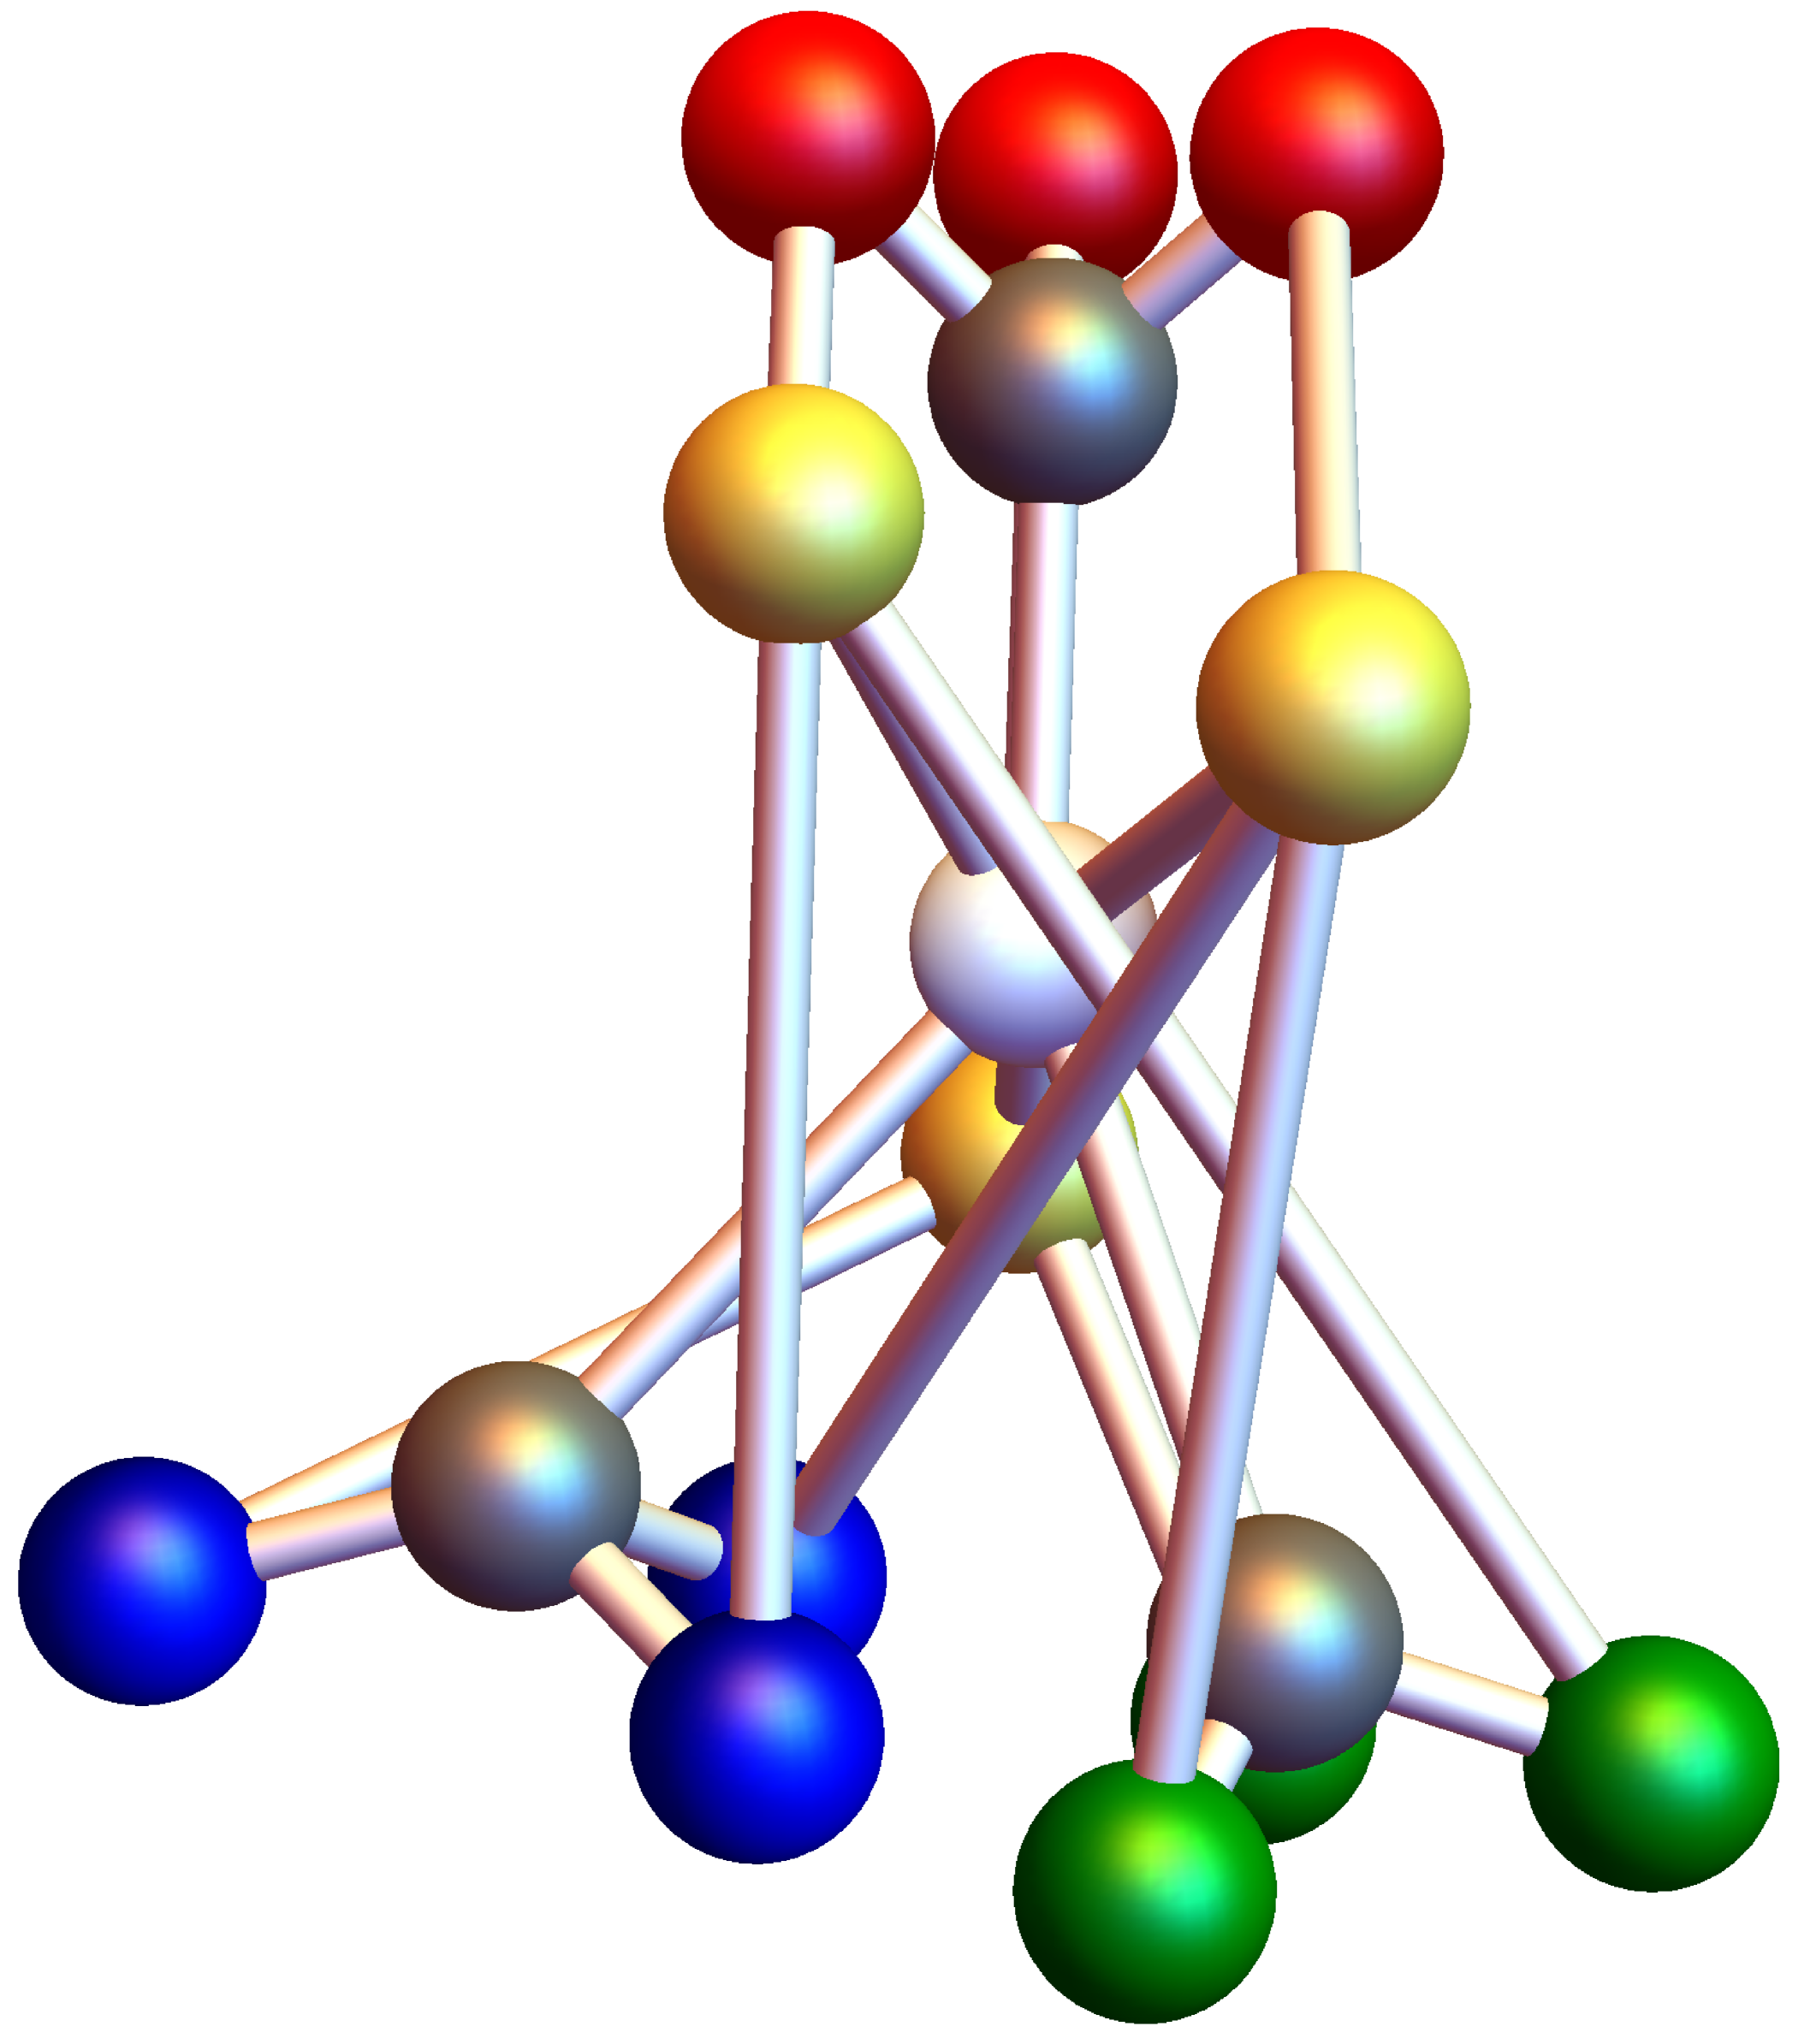
\includegraphics[trim=0mm 0 0 0mm, width=0.5\textwidth]{Images/switch_square}
	\end{center}
	\begin{itemize}
		\item Transport part of an entangled pair along the network
		\item Entangle separated parts of a system
		\item Quantum teleportation as transportation scheme
	\end{itemize}
\end{frame}}

\begin{center}
	\includeslide{graphs}
\end{center}

\noindent text


\mode<presentation>{\begin{frame}{Examples}\label{adjexamples}
	\begin{center}
		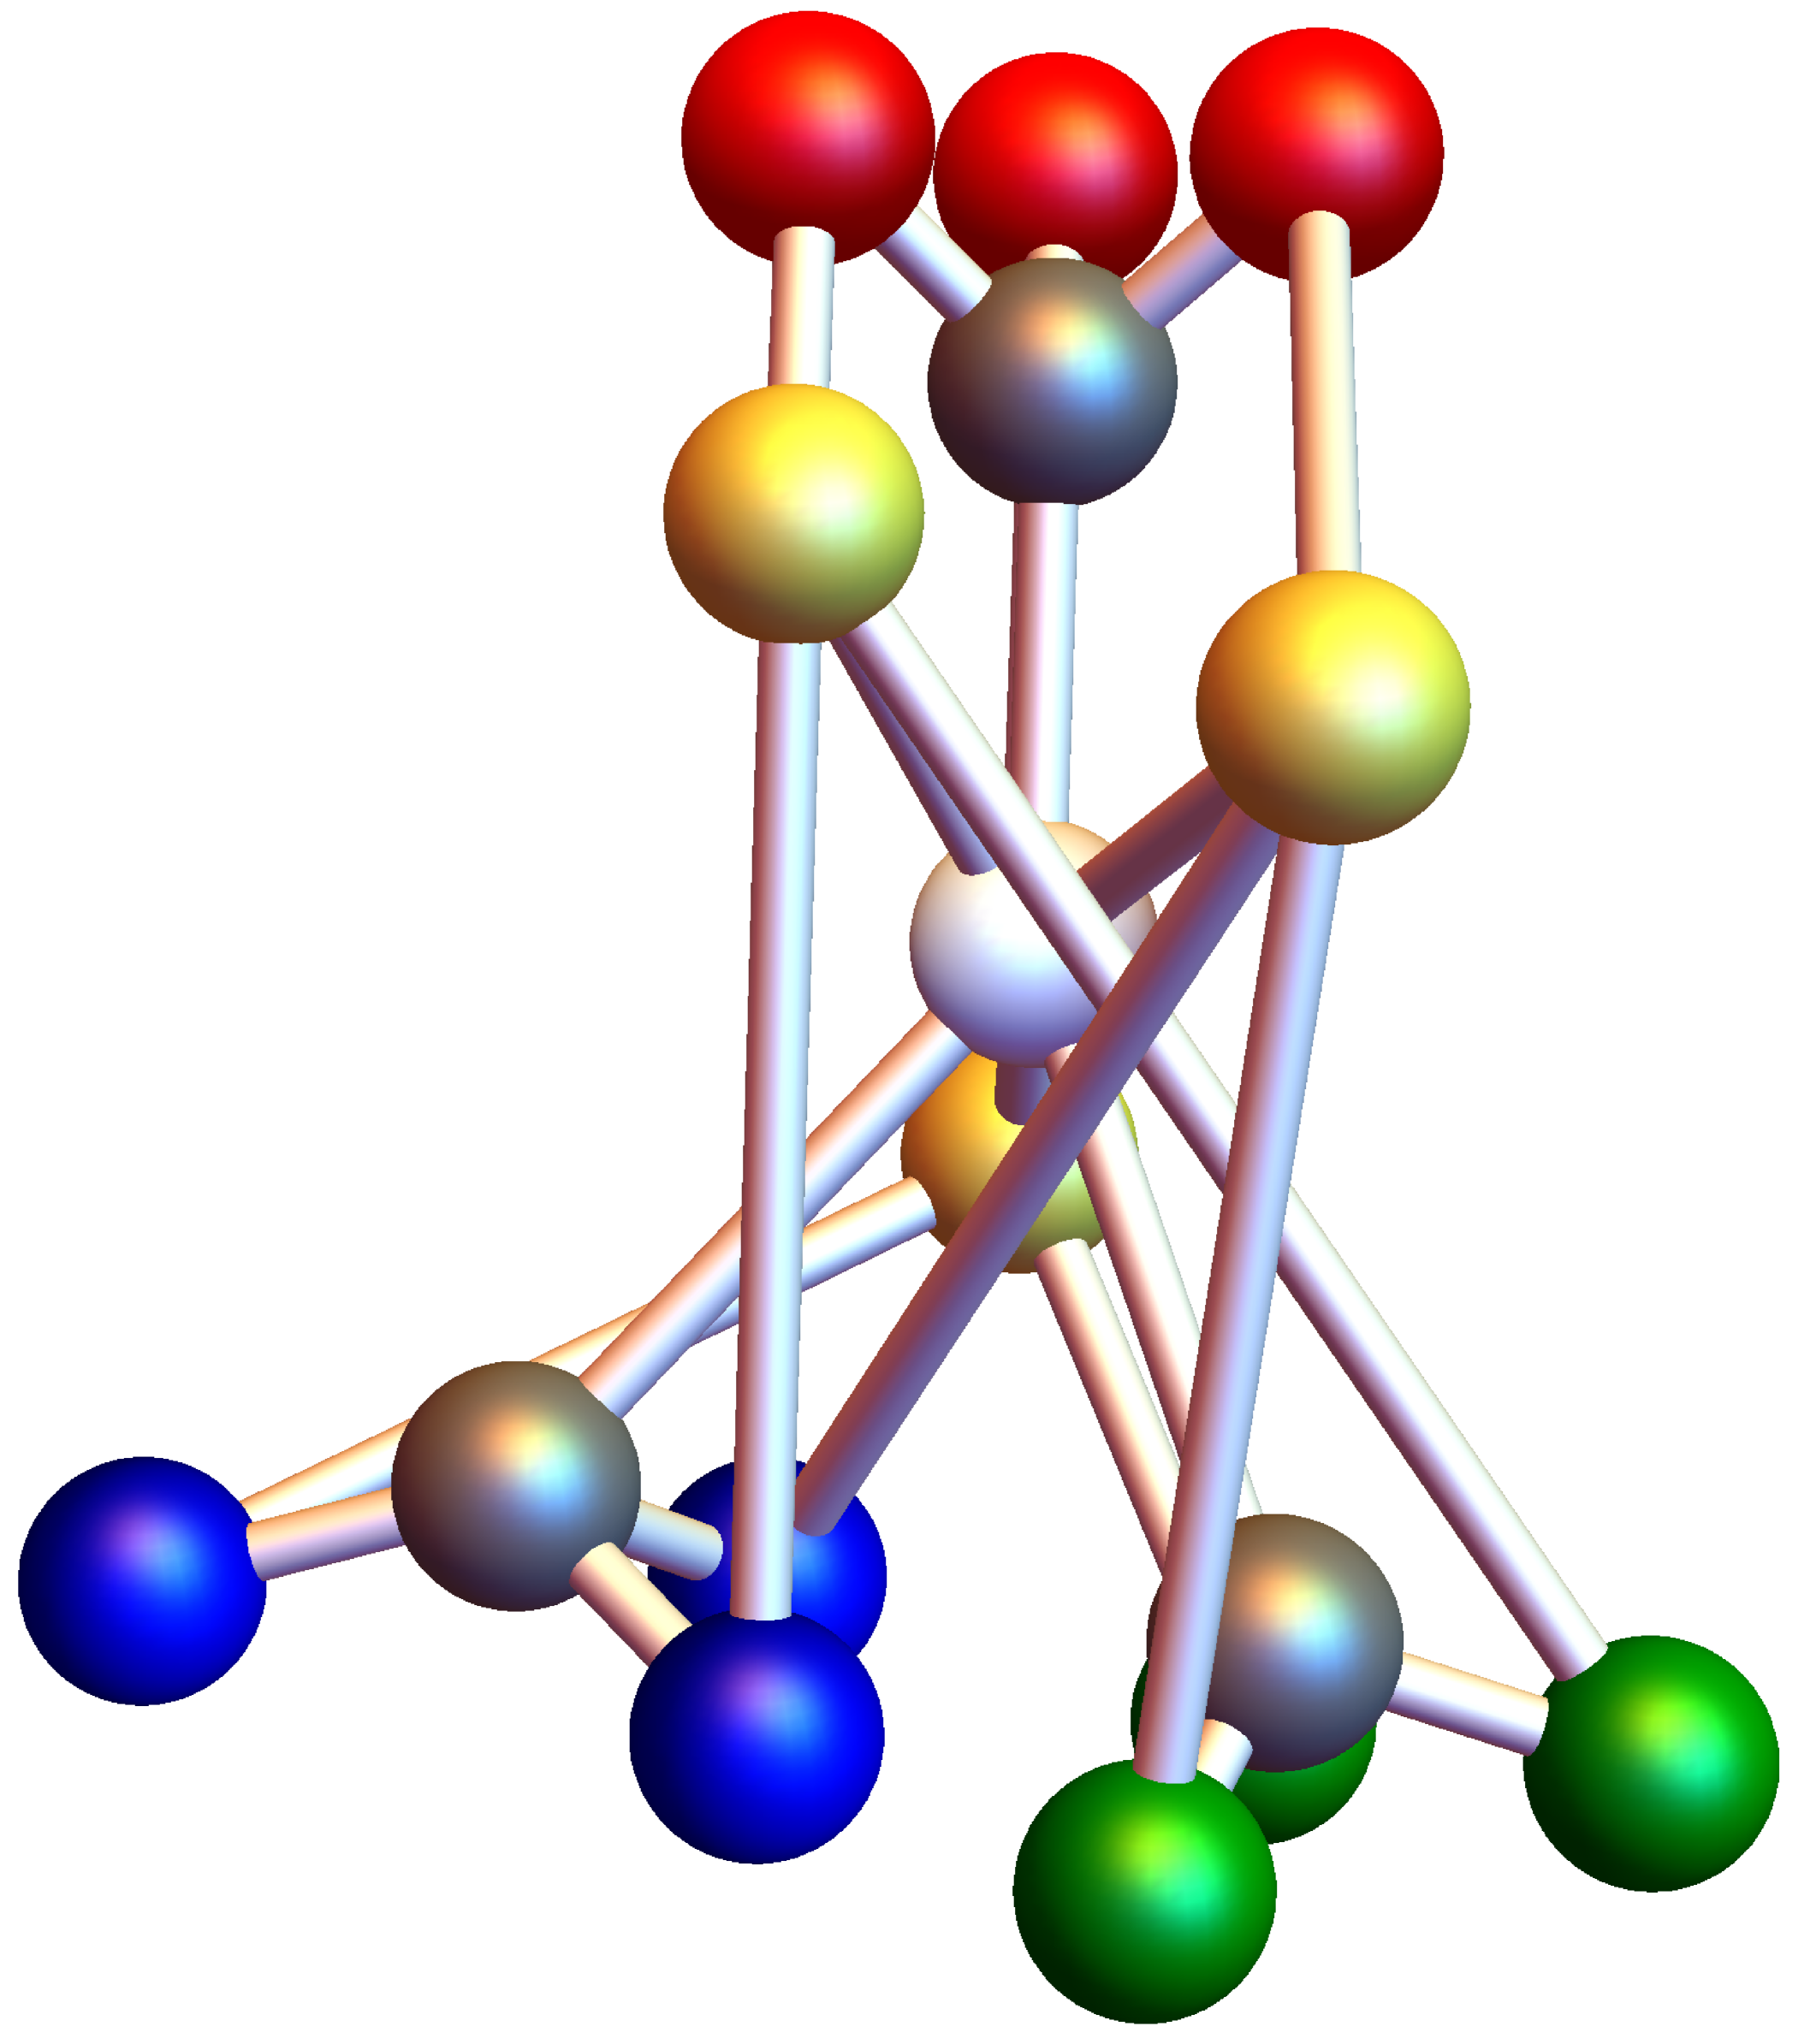
\includegraphics[trim=0mm 0 0 0mm, width=0.5\textwidth]{Images/switch_square}
	\end{center}
	\begin{itemize}
		\item Transport part of an entangled pair along the network
		\item Entangle separated parts of a system
		\item Quantum teleportation as transportation scheme
	\end{itemize}
\end{frame}}

\begin{center}
	\includeslide{adjexamples}
\end{center}

\noindent text


\mode<presentation>{\begin{frame}{Identifying PST Graphs}\label{identifyPST}
	\begin{center}
		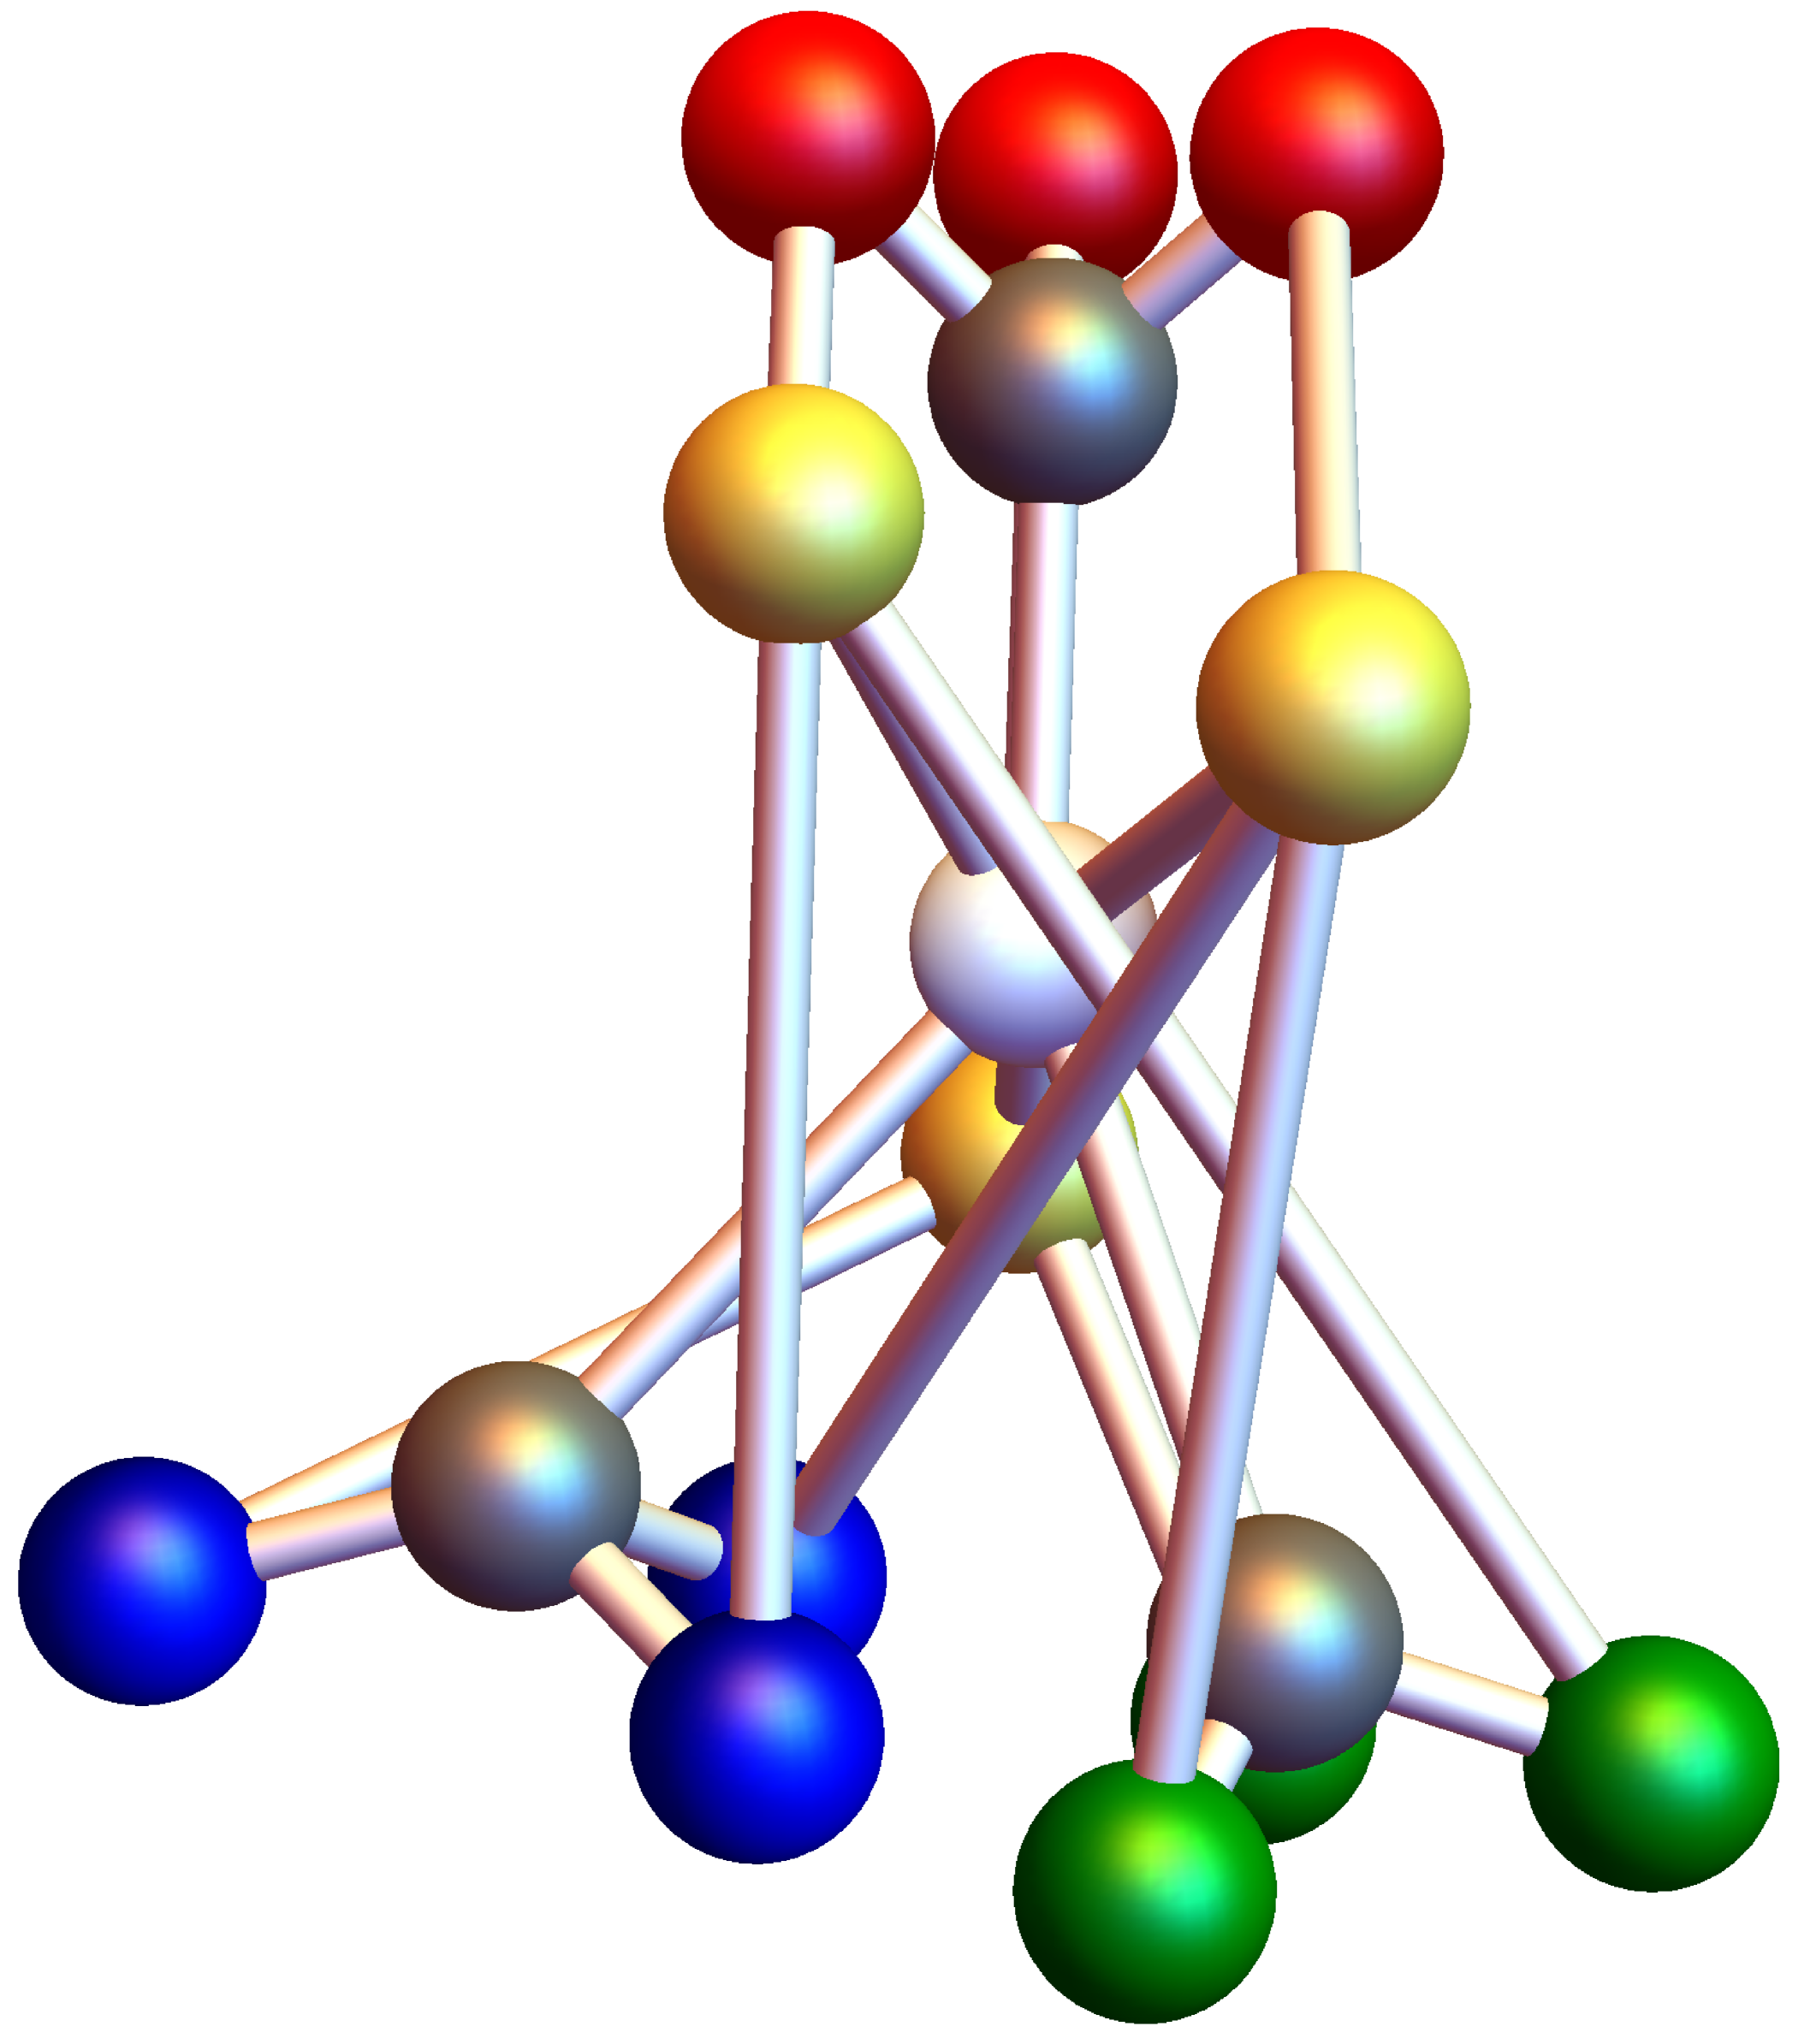
\includegraphics[trim=0mm 0 0 0mm, width=0.5\textwidth]{Images/switch_square}
	\end{center}
	\begin{itemize}
		\item Transport part of an entangled pair along the network
		\item Entangle separated parts of a system
		\item Quantum teleportation as transportation scheme
	\end{itemize}
\end{frame}}

\begin{center}
	\includeslide{identifyPST}
\end{center}

\noindent text


\mode<presentation>{\begin{frame}{Quantum Routing}\label{routing}
	\begin{center}
		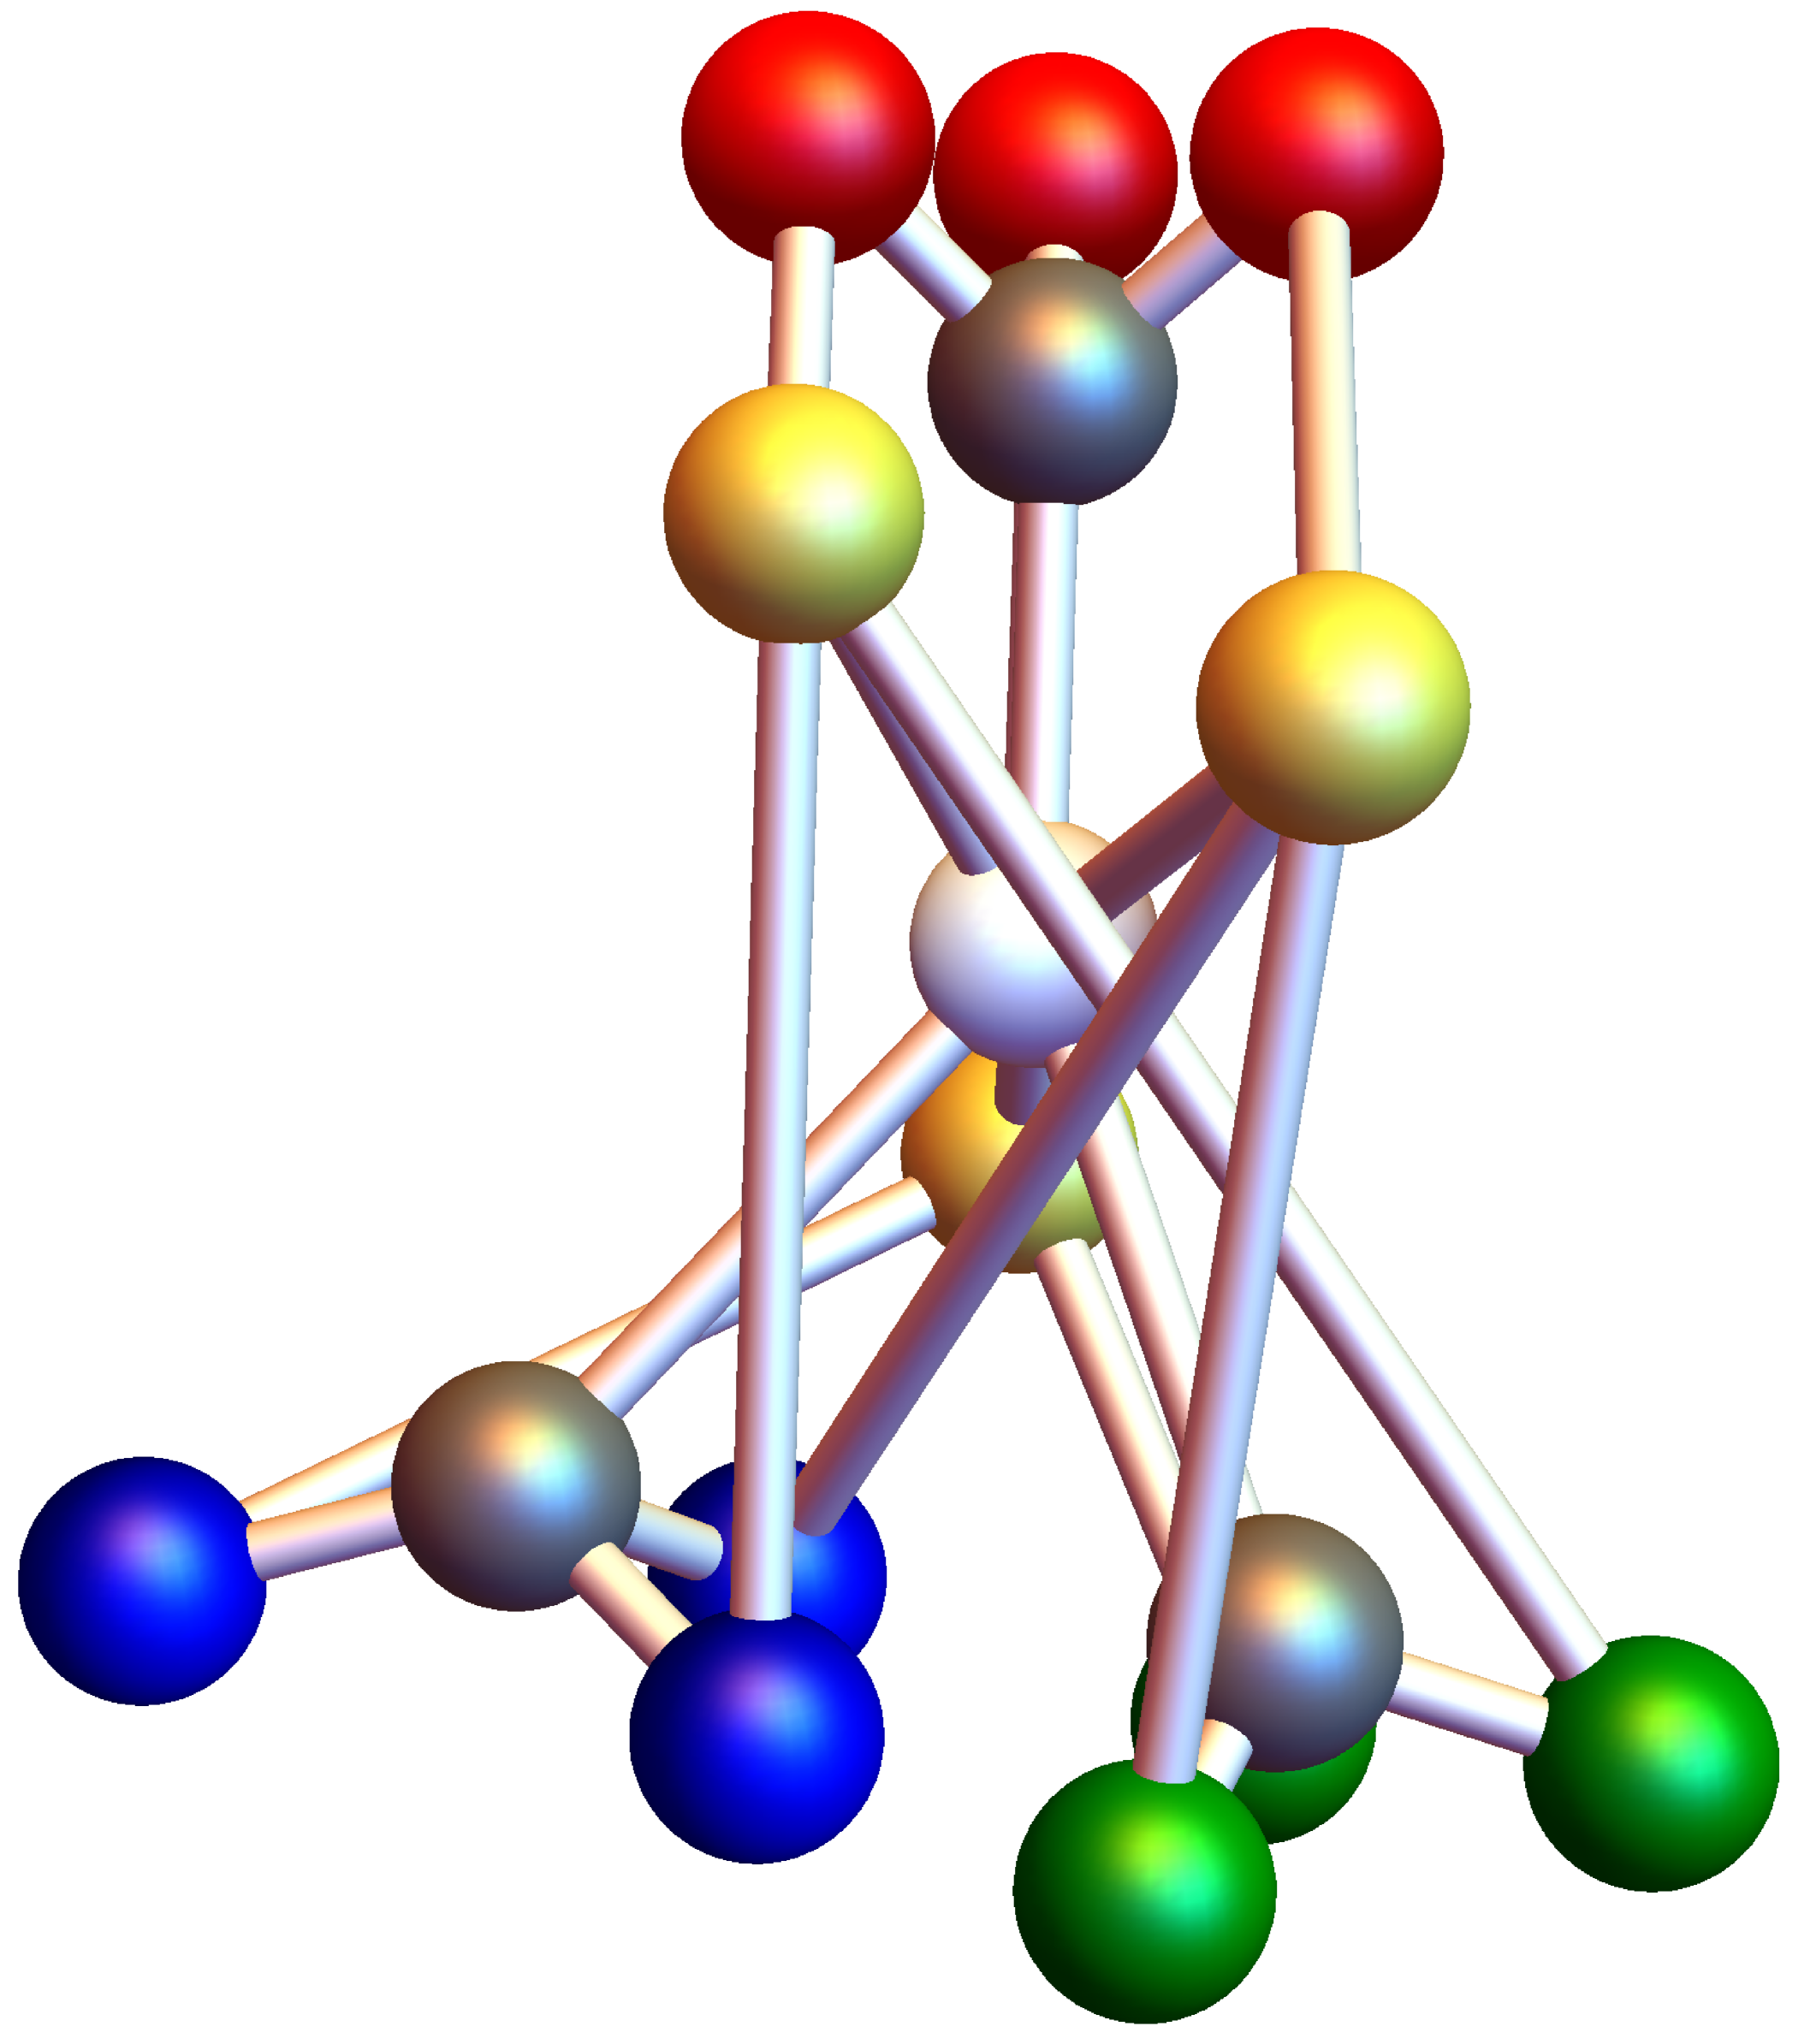
\includegraphics[trim=0mm 0 0 0mm, width=0.5\textwidth]{Images/switch_square}
	\end{center}
	\begin{itemize}
		\item Transport part of an entangled pair along the network
		\item Entangle separated parts of a system
		\item Quantum teleportation as transportation scheme
	\end{itemize}
\end{frame}}

\begin{center}
	\includeslide{routing}
\end{center}

\noindent text


\mode<presentation>{\begin{frame}{Graph Product}\label{graphproduct}
	\begin{center}
		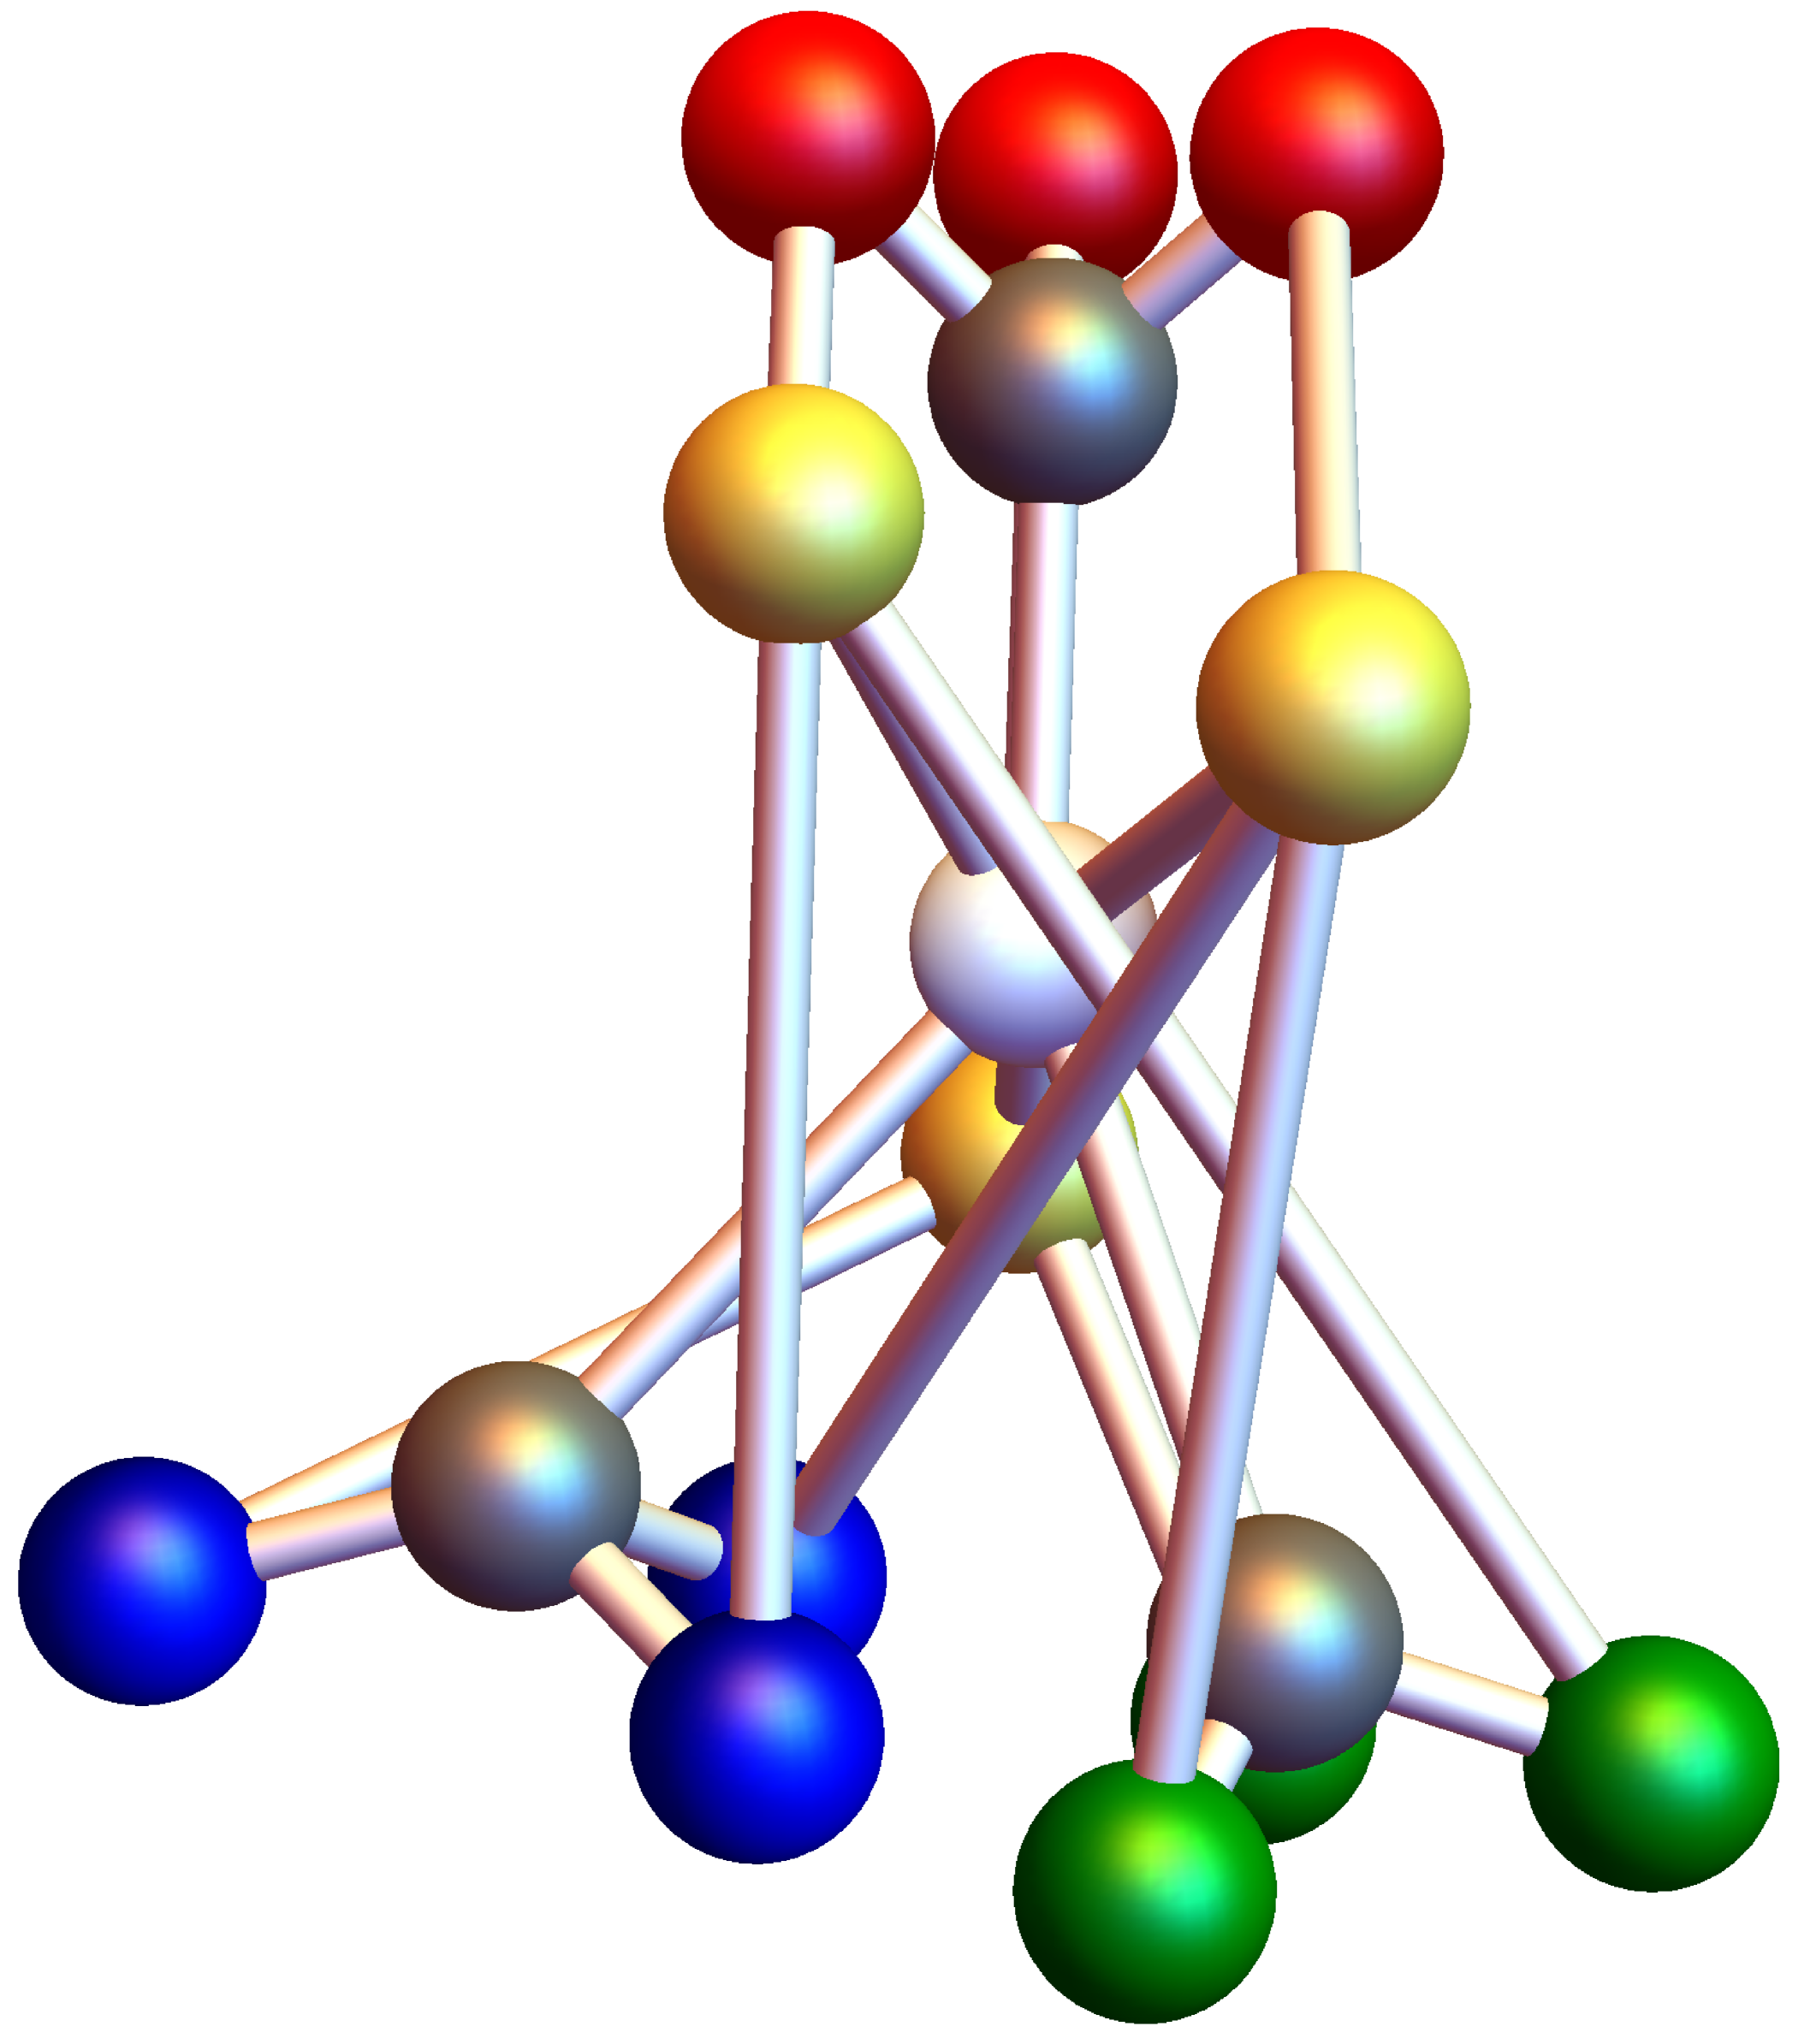
\includegraphics[trim=0mm 0 0 0mm, width=0.5\textwidth]{Images/switch_square}
	\end{center}
	\begin{itemize}
		\item Transport part of an entangled pair along the network
		\item Entangle separated parts of a system
		\item Quantum teleportation as transportation scheme
	\end{itemize}
\end{frame}}

\begin{center}
	\includeslide{graphproduct}
\end{center}

\noindent text


\mode<presentation>{\begin{frame}{Higher Excitation Spaces}\label{hes}
	\begin{center}
		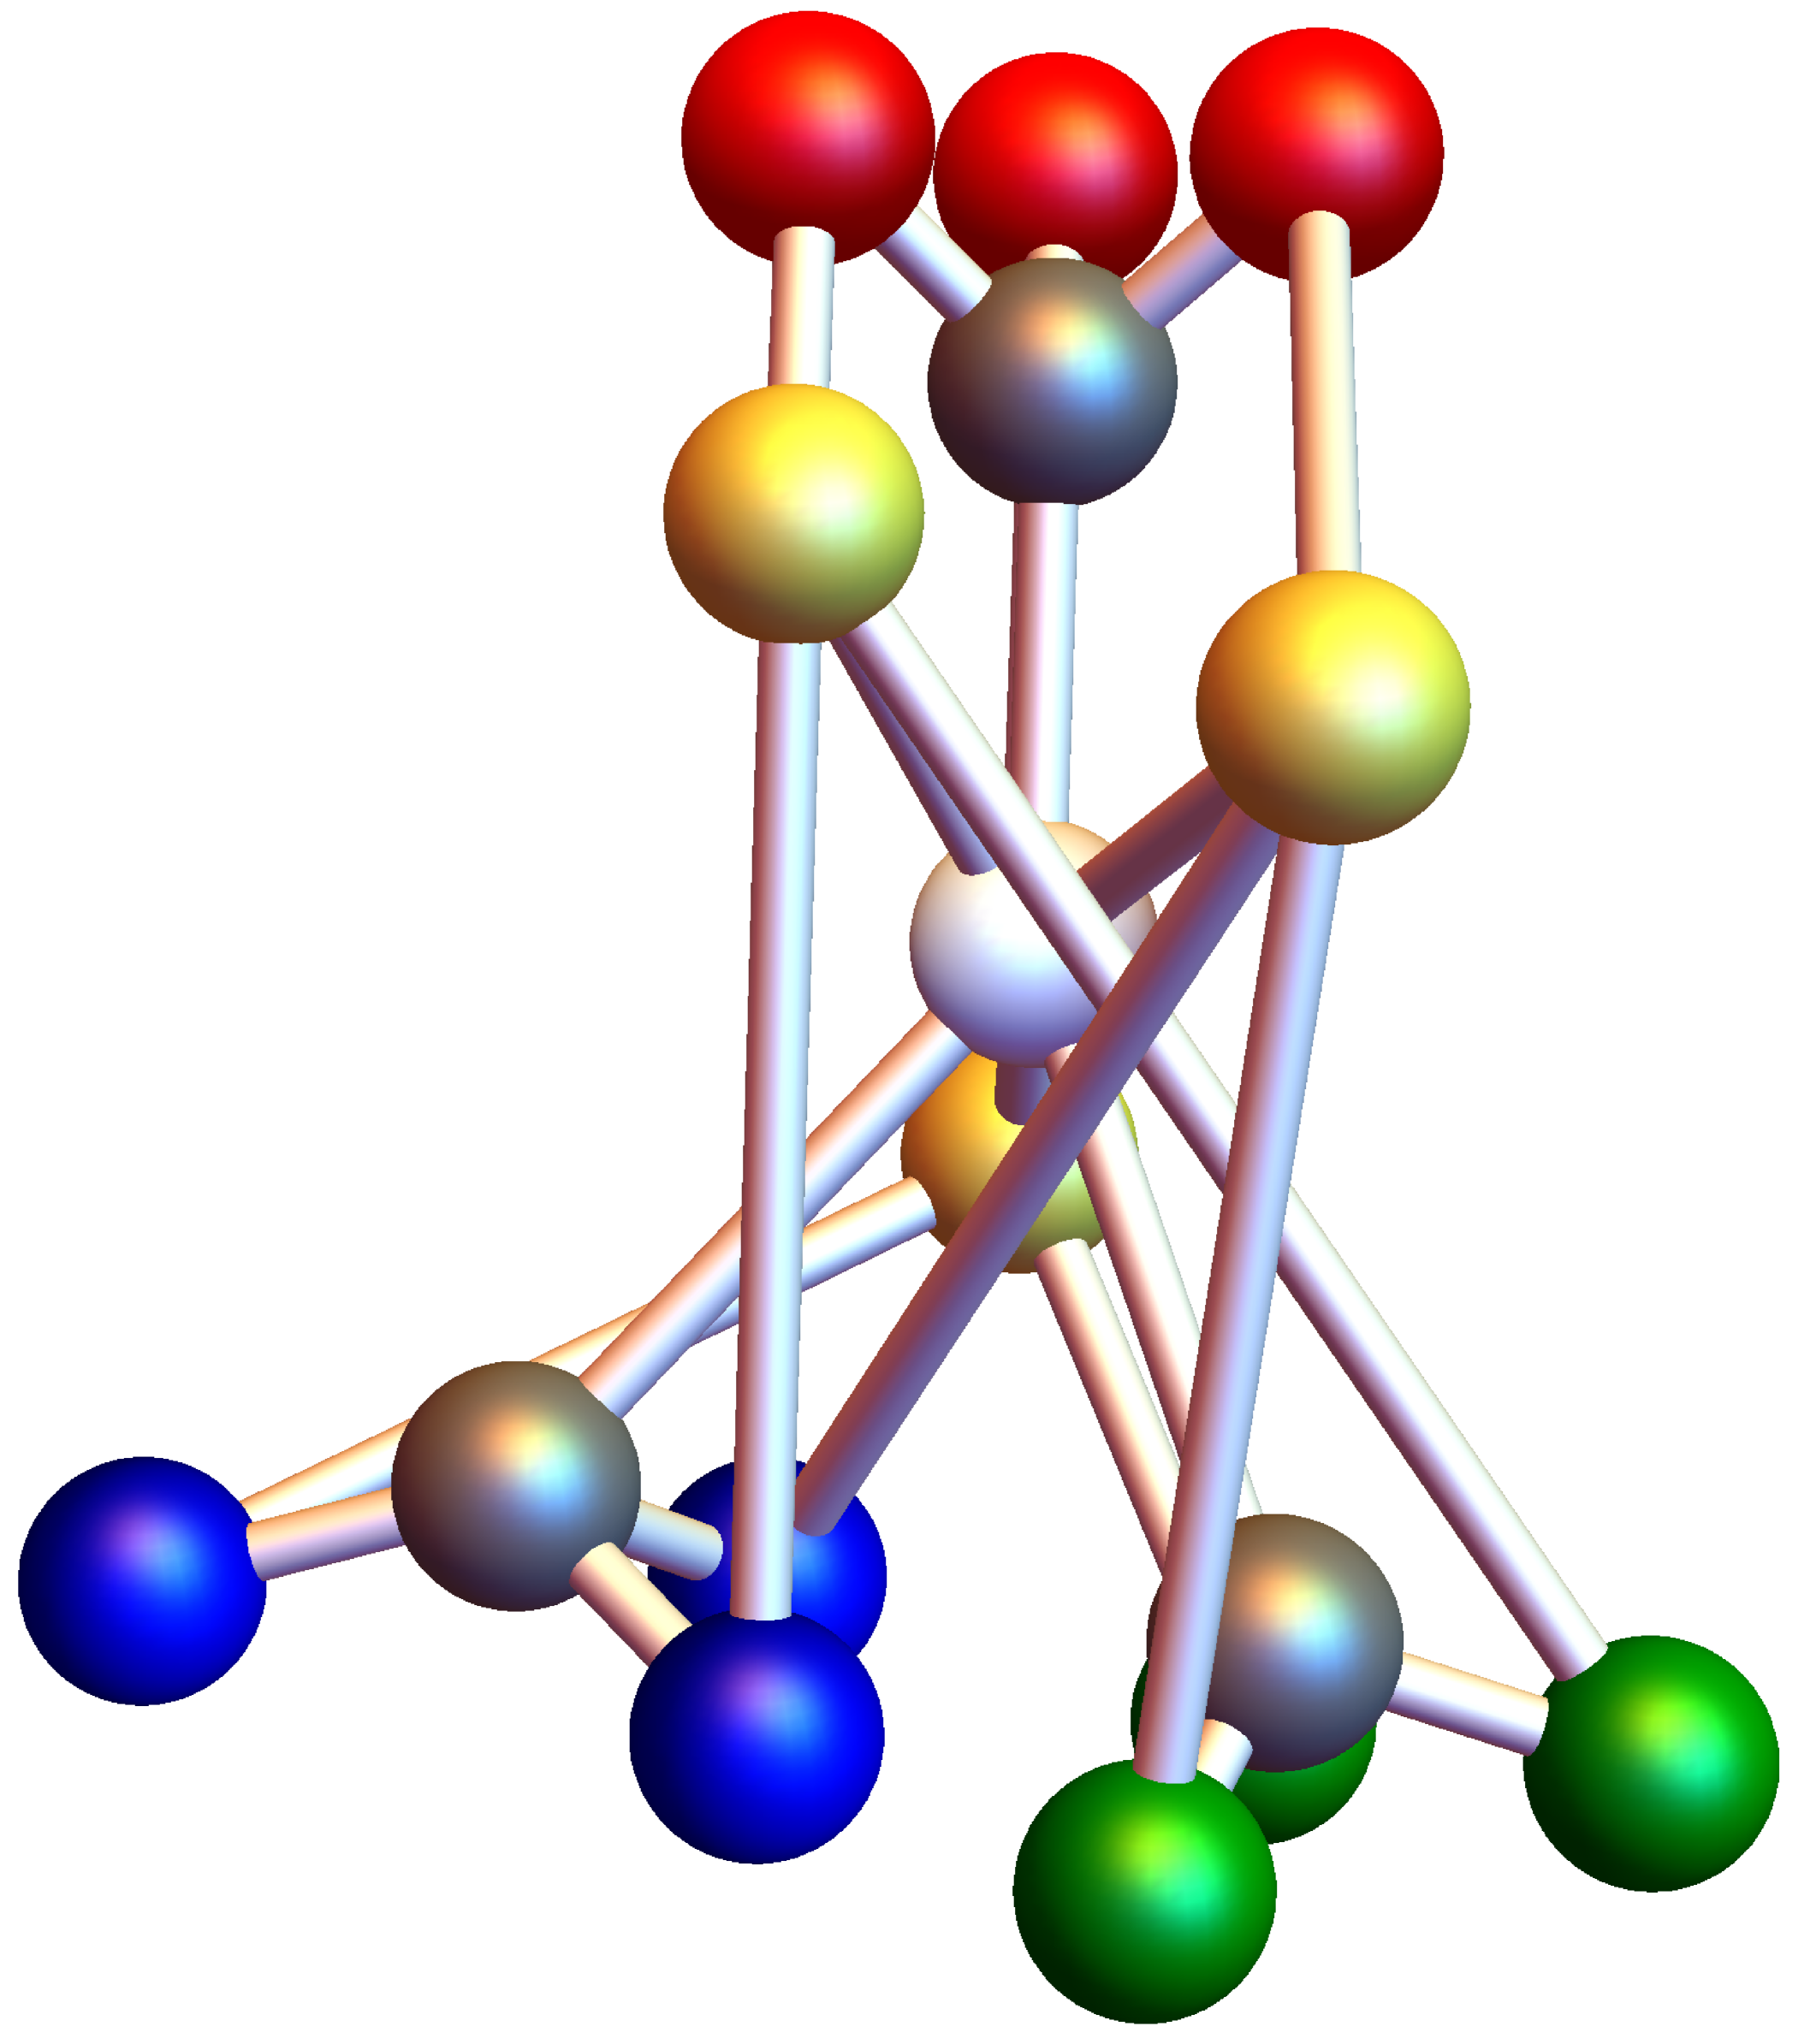
\includegraphics[trim=0mm 0 0 0mm, width=0.5\textwidth]{Images/switch_square}
	\end{center}
	\begin{itemize}
		\item Transport part of an entangled pair along the network
		\item Entangle separated parts of a system
		\item Quantum teleportation as transportation scheme
	\end{itemize}
\end{frame}}

\begin{center}
	\includeslide{hes}
\end{center}

\noindent text


\mode<presentation>{\begin{frame}{Renormalization}\label{renormalization}
	\begin{center}
		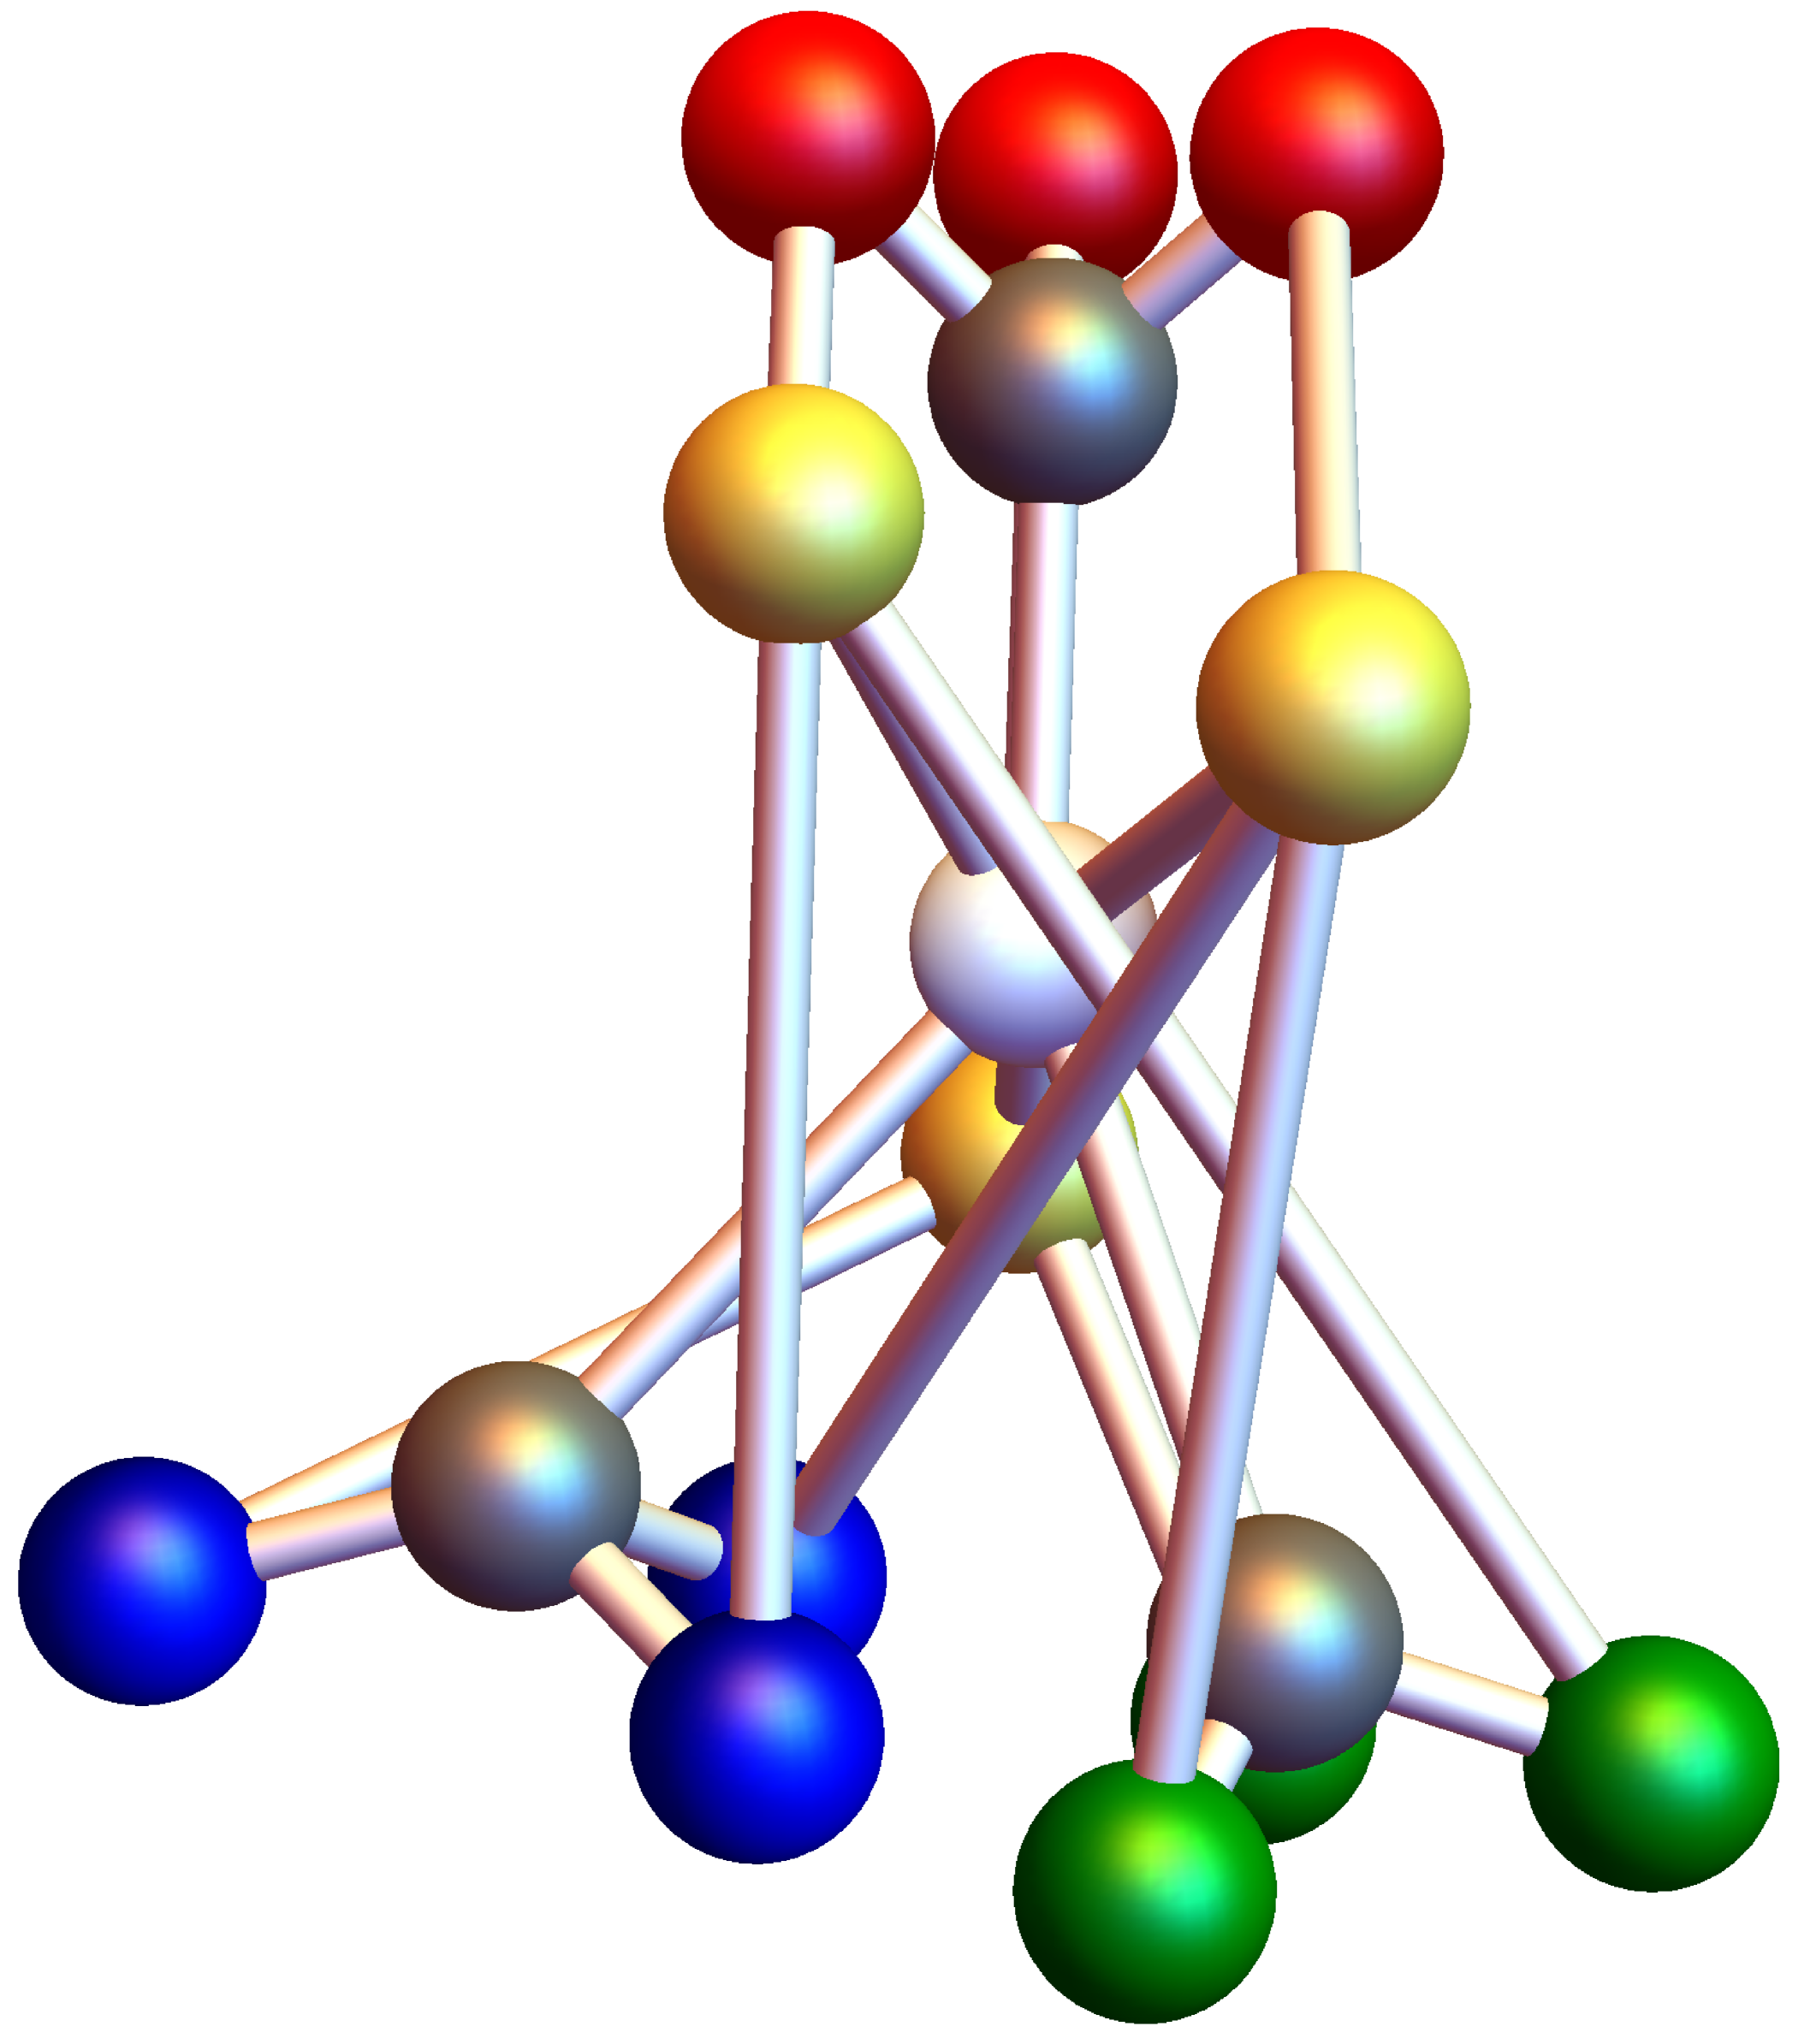
\includegraphics[trim=0mm 0 0 0mm, width=0.5\textwidth]{Images/switch_square}
	\end{center}
	\begin{itemize}
		\item Transport part of an entangled pair along the network
		\item Entangle separated parts of a system
		\item Quantum teleportation as transportation scheme
	\end{itemize}
\end{frame}}

\begin{center}
	\includeslide{renormalization}
\end{center}

\noindent text


\mode<presentation>{\begin{frame}{The Method}\label{method}
	\begin{center}
		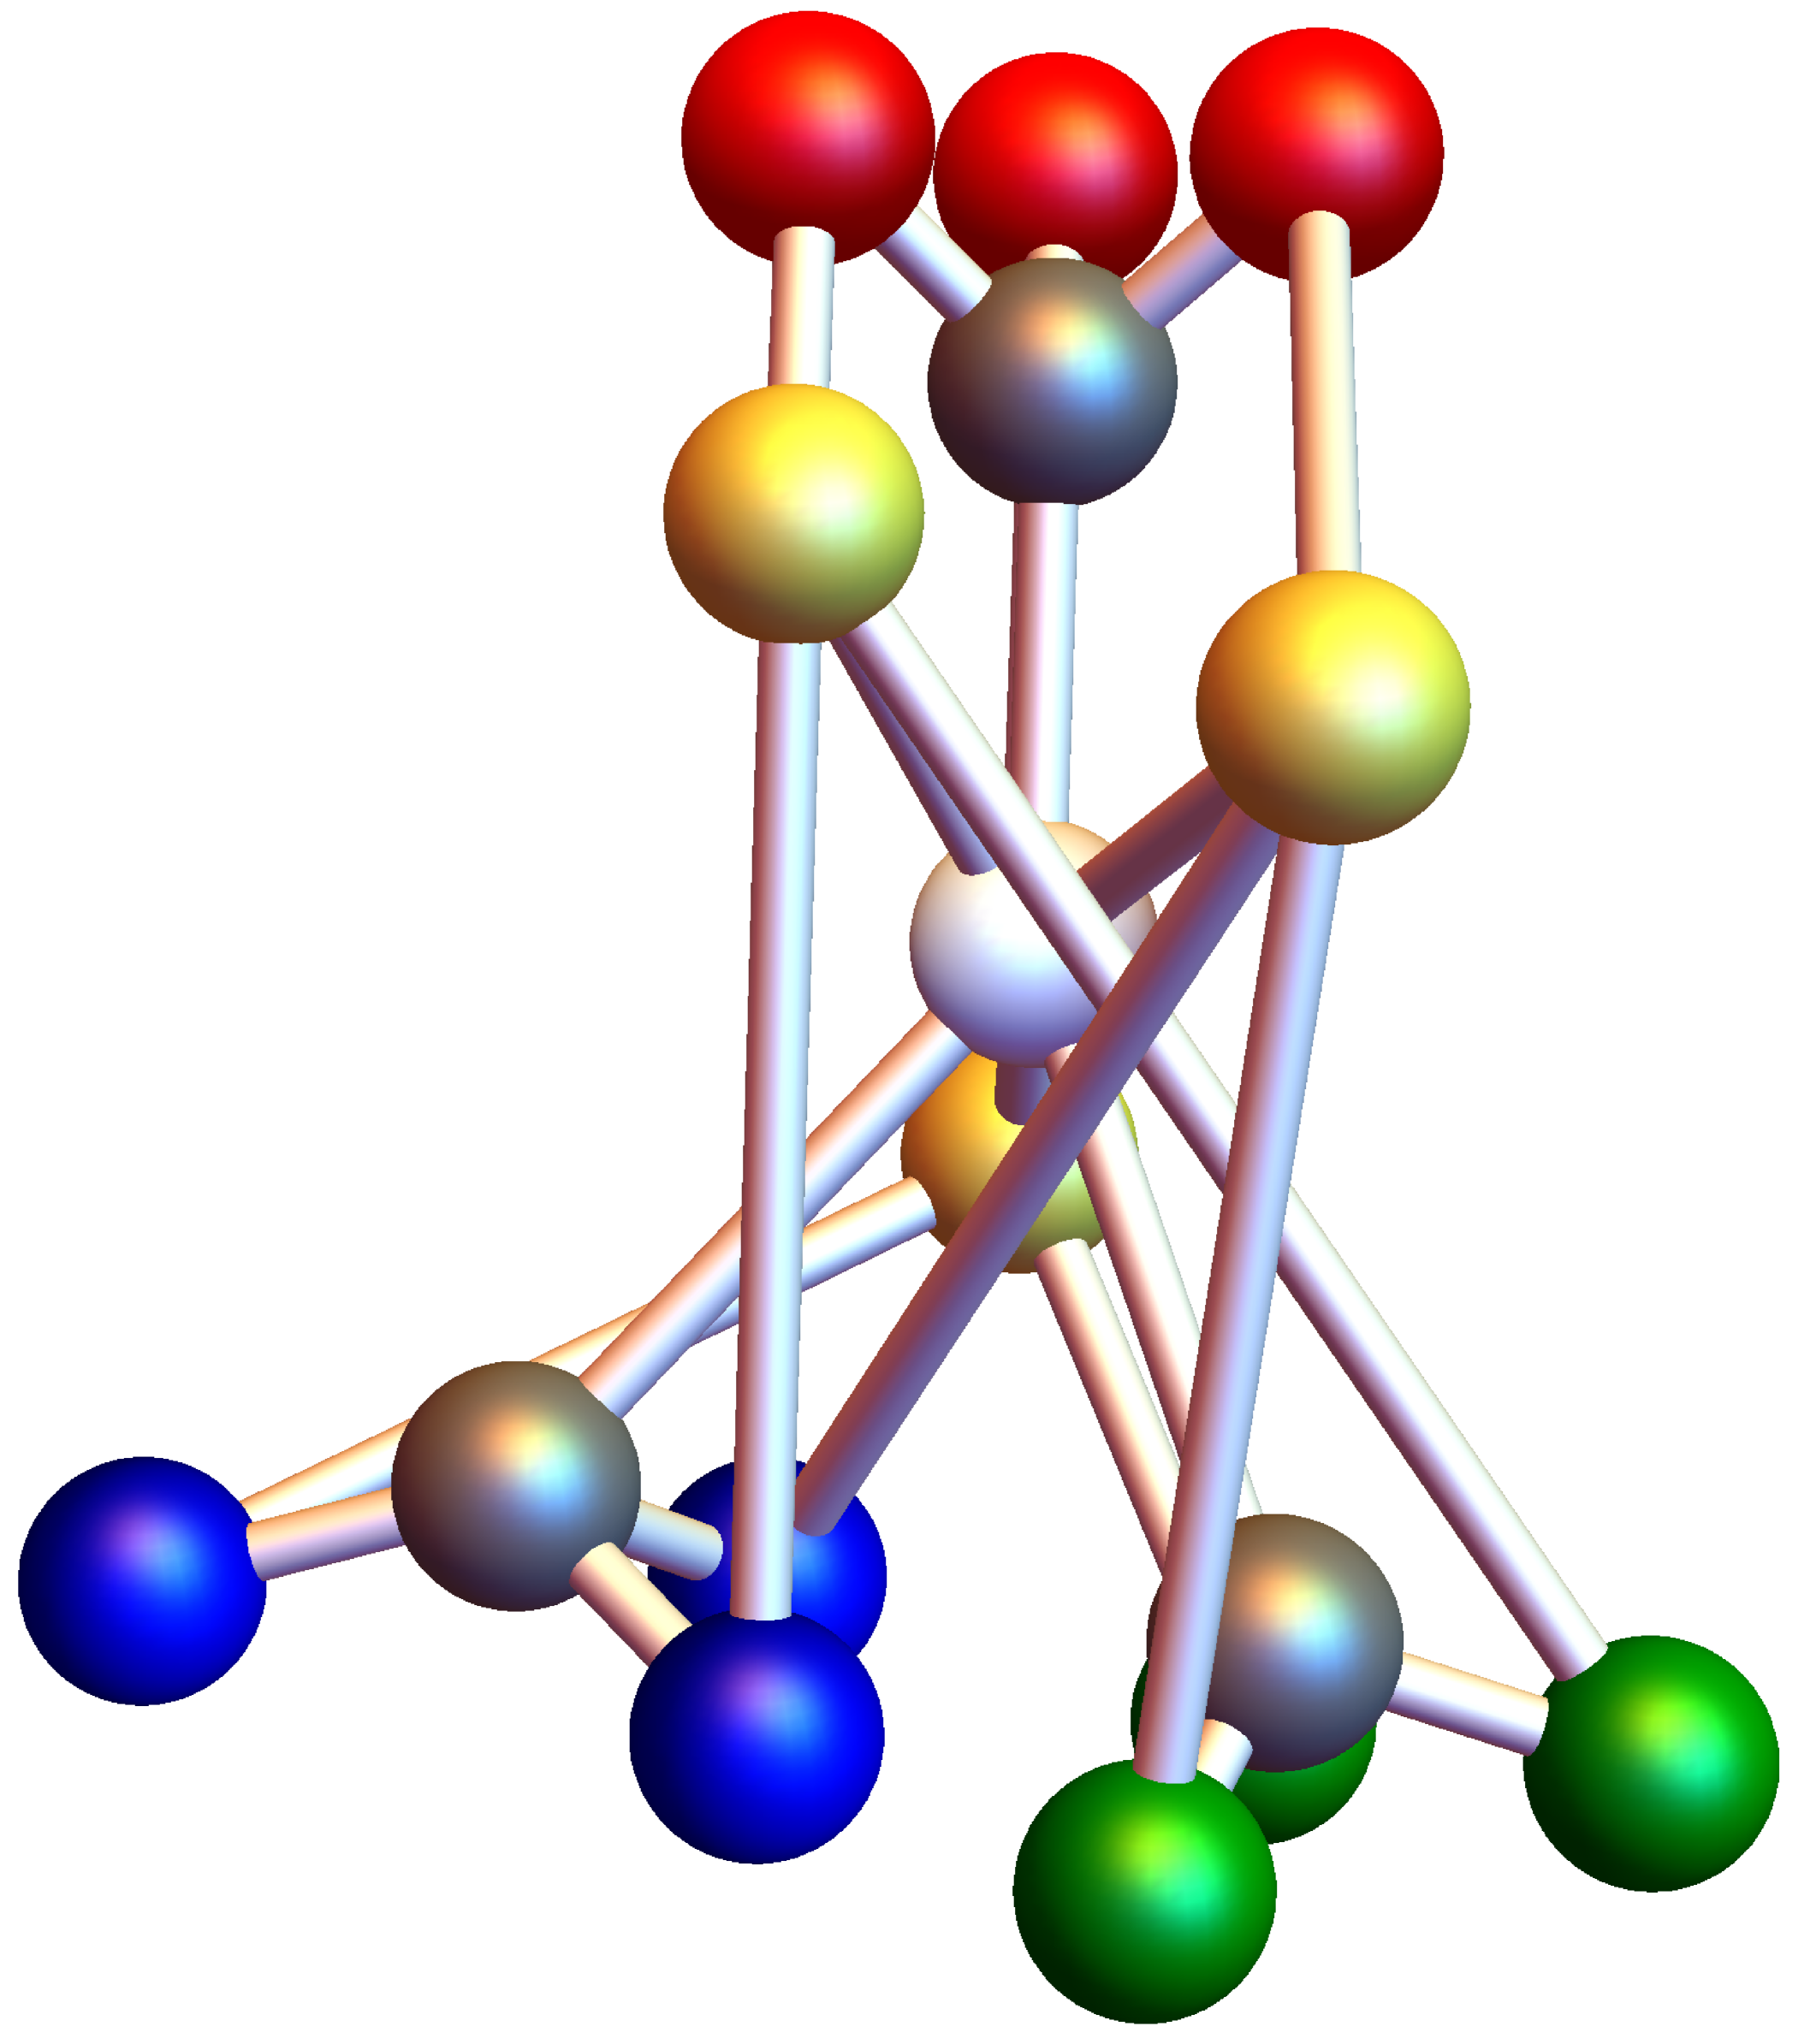
\includegraphics[trim=0mm 0 0 0mm, width=0.5\textwidth]{Images/switch_square}
	\end{center}
	\begin{itemize}
		\item Transport part of an entangled pair along the network
		\item Entangle separated parts of a system
		\item Quantum teleportation as transportation scheme
	\end{itemize}
\end{frame}}

\begin{center}
	\includeslide{method}
\end{center}

\noindent text


\mode<presentation>{\begin{frame}{Conclusion}\label{conclusion}
	\begin{center}
		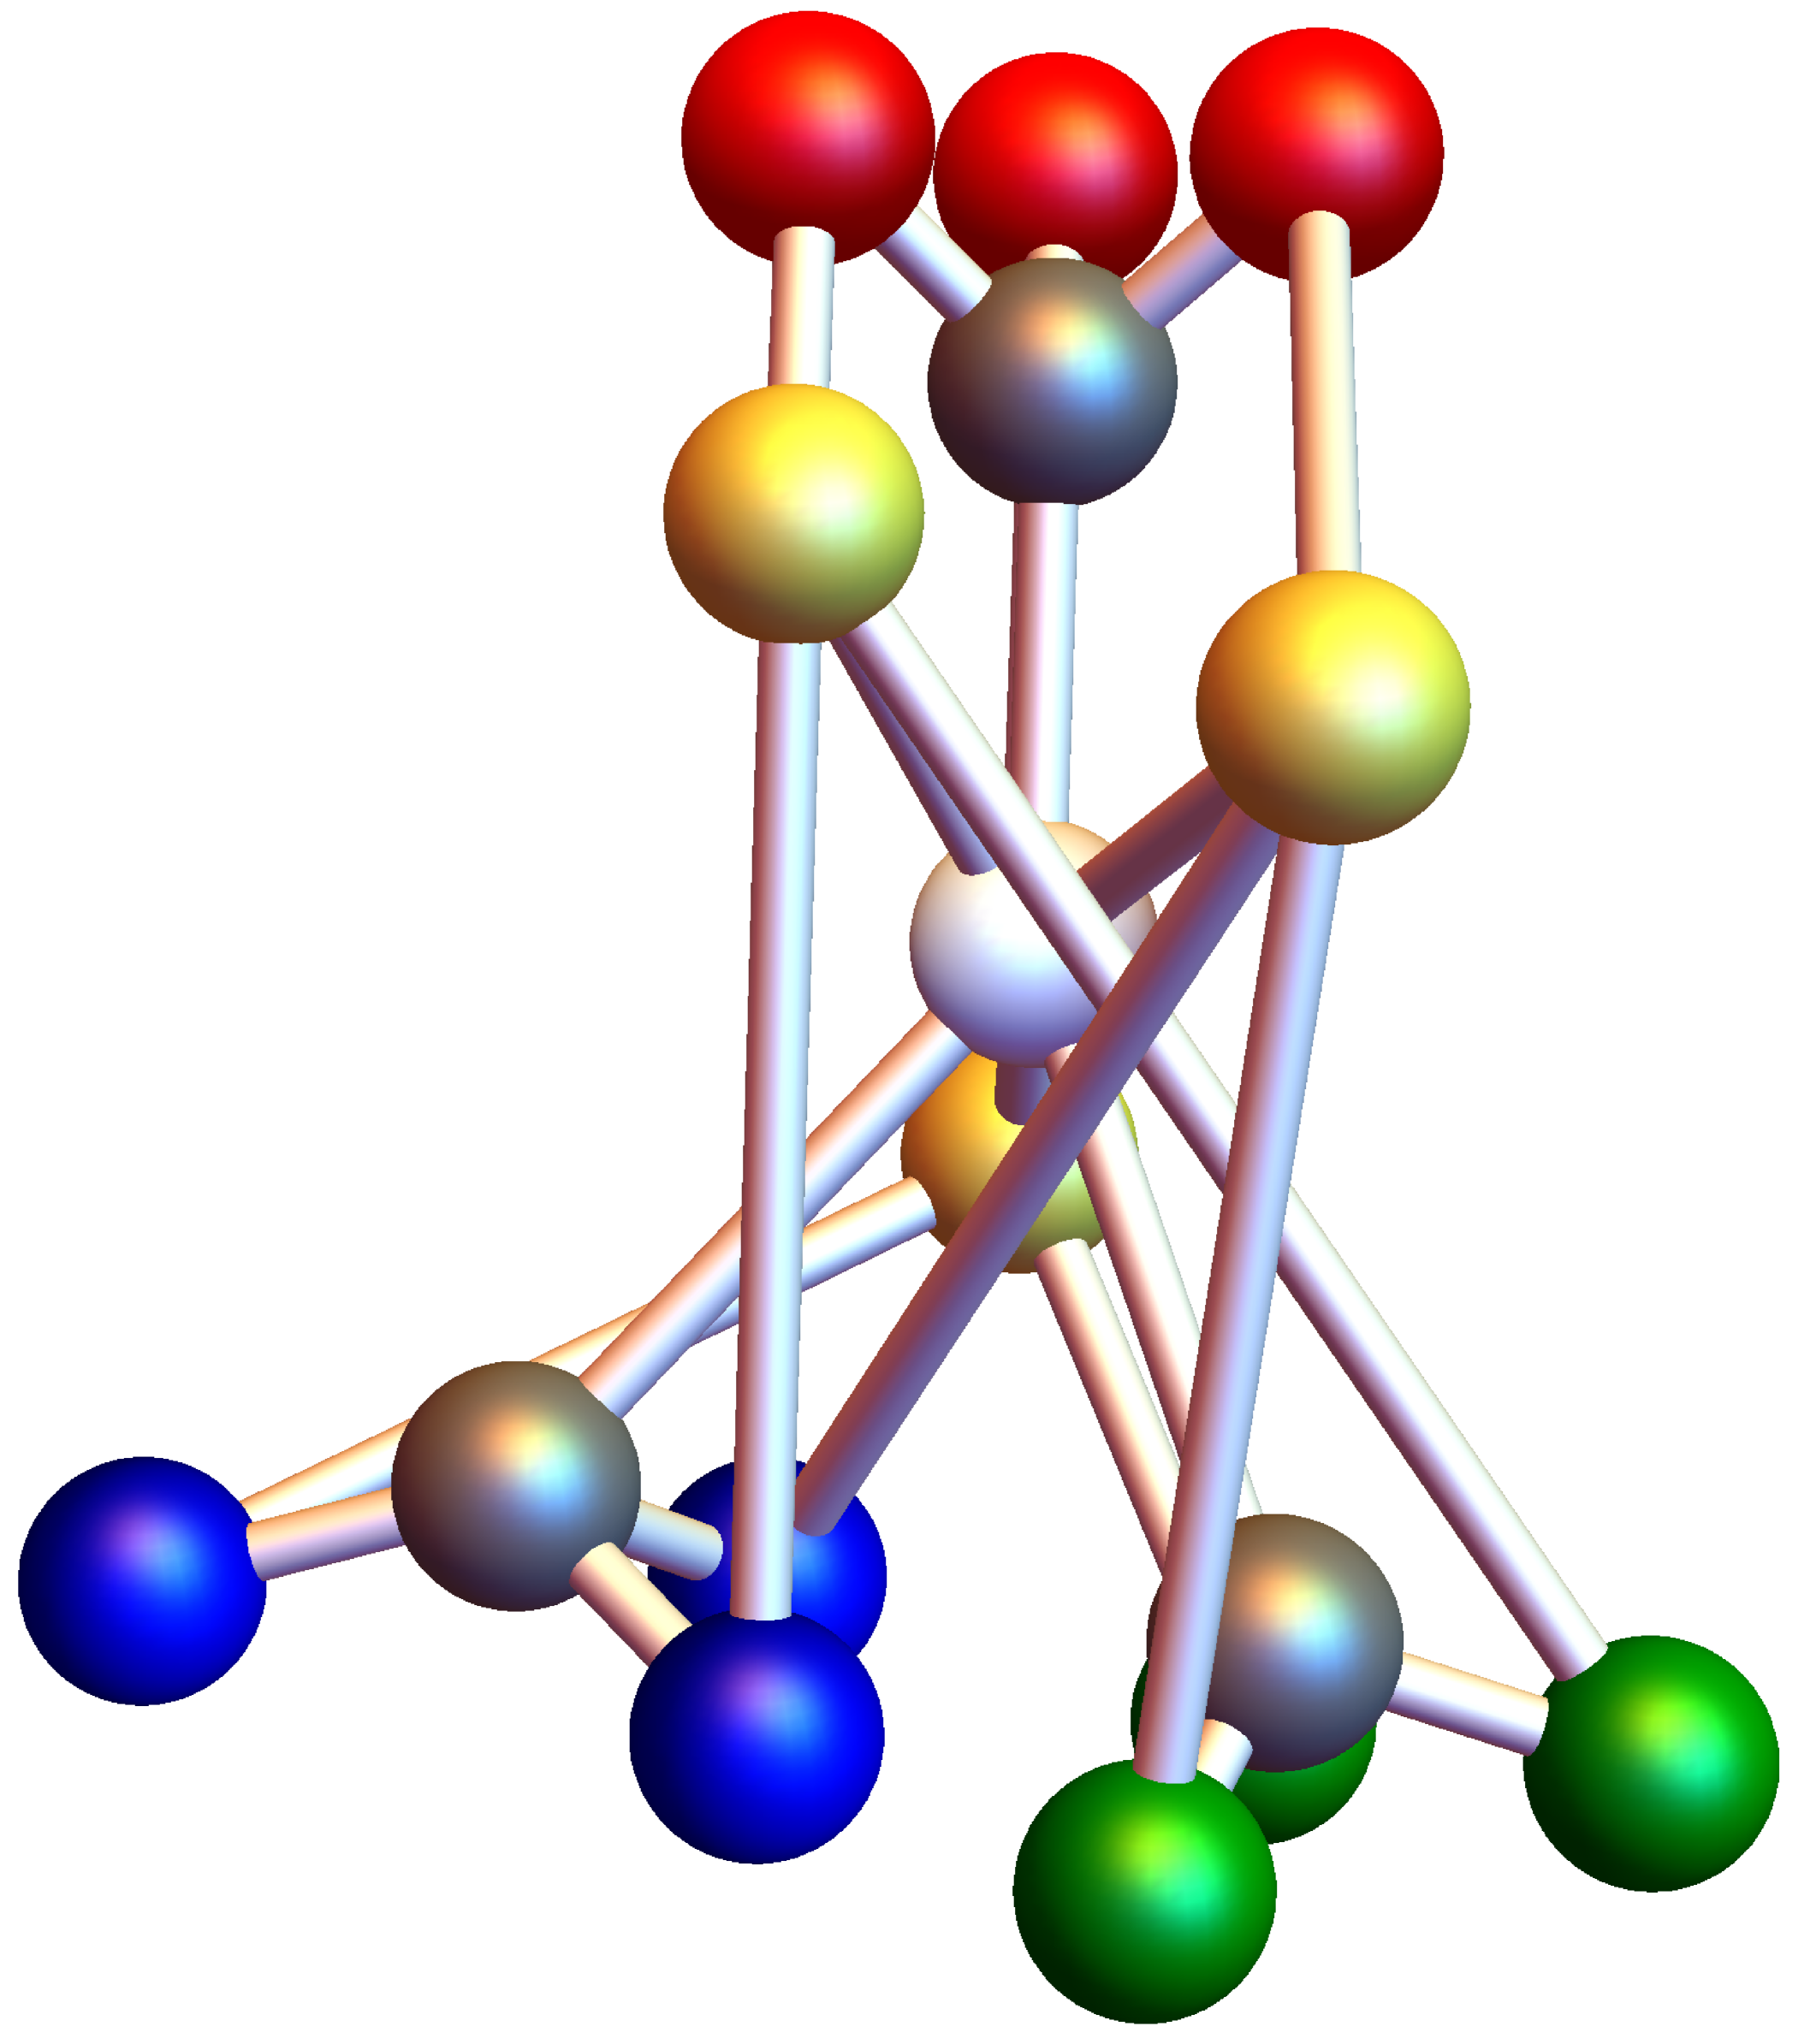
\includegraphics[trim=0mm 0 0 0mm, width=0.5\textwidth]{Images/switch_square}
	\end{center}
	\begin{itemize}
		\item Transport part of an entangled pair along the network
		\item Entangle separated parts of a system
		\item Quantum teleportation as transportation scheme
	\end{itemize}
\end{frame}}

\begin{center}
	\includeslide{conclusion}
\end{center}

\noindent text



\end{document}
